% Options for packages loaded elsewhere
\PassOptionsToPackage{unicode}{hyperref}
\PassOptionsToPackage{hyphens}{url}
\PassOptionsToPackage{dvipsnames,svgnames,x11names}{xcolor}
%
\documentclass[
  letterpaper,
  authoryear,
  preprint,
  3p]{elsarticle}

\usepackage{amsmath,amssymb}
\usepackage{lmodern}
\usepackage{iftex}
\ifPDFTeX
  \usepackage[T1]{fontenc}
  \usepackage[utf8]{inputenc}
  \usepackage{textcomp} % provide euro and other symbols
\else % if luatex or xetex
  \usepackage{unicode-math}
  \defaultfontfeatures{Scale=MatchLowercase}
  \defaultfontfeatures[\rmfamily]{Ligatures=TeX,Scale=1}
\fi
% Use upquote if available, for straight quotes in verbatim environments
\IfFileExists{upquote.sty}{\usepackage{upquote}}{}
\IfFileExists{microtype.sty}{% use microtype if available
  \usepackage[]{microtype}
  \UseMicrotypeSet[protrusion]{basicmath} % disable protrusion for tt fonts
}{}
\makeatletter
\@ifundefined{KOMAClassName}{% if non-KOMA class
  \IfFileExists{parskip.sty}{%
    \usepackage{parskip}
  }{% else
    \setlength{\parindent}{0pt}
    \setlength{\parskip}{6pt plus 2pt minus 1pt}}
}{% if KOMA class
  \KOMAoptions{parskip=half}}
\makeatother
\usepackage{xcolor}
\setlength{\emergencystretch}{3em} % prevent overfull lines
\setcounter{secnumdepth}{5}
% Make \paragraph and \subparagraph free-standing
\ifx\paragraph\undefined\else
  \let\oldparagraph\paragraph
  \renewcommand{\paragraph}[1]{\oldparagraph{#1}\mbox{}}
\fi
\ifx\subparagraph\undefined\else
  \let\oldsubparagraph\subparagraph
  \renewcommand{\subparagraph}[1]{\oldsubparagraph{#1}\mbox{}}
\fi


\providecommand{\tightlist}{%
  \setlength{\itemsep}{0pt}\setlength{\parskip}{0pt}}\usepackage{longtable,booktabs,array}
\usepackage{calc} % for calculating minipage widths
% Correct order of tables after \paragraph or \subparagraph
\usepackage{etoolbox}
\makeatletter
\patchcmd\longtable{\par}{\if@noskipsec\mbox{}\fi\par}{}{}
\makeatother
% Allow footnotes in longtable head/foot
\IfFileExists{footnotehyper.sty}{\usepackage{footnotehyper}}{\usepackage{footnote}}
\makesavenoteenv{longtable}
\usepackage{graphicx}
\makeatletter
\def\maxwidth{\ifdim\Gin@nat@width>\linewidth\linewidth\else\Gin@nat@width\fi}
\def\maxheight{\ifdim\Gin@nat@height>\textheight\textheight\else\Gin@nat@height\fi}
\makeatother
% Scale images if necessary, so that they will not overflow the page
% margins by default, and it is still possible to overwrite the defaults
% using explicit options in \includegraphics[width, height, ...]{}
\setkeys{Gin}{width=\maxwidth,height=\maxheight,keepaspectratio}
% Set default figure placement to htbp
\makeatletter
\def\fps@figure{htbp}
\makeatother
\newlength{\cslhangindent}
\setlength{\cslhangindent}{1.5em}
\newlength{\csllabelwidth}
\setlength{\csllabelwidth}{3em}
\newlength{\cslentryspacingunit} % times entry-spacing
\setlength{\cslentryspacingunit}{\parskip}
\newenvironment{CSLReferences}[2] % #1 hanging-ident, #2 entry spacing
 {% don't indent paragraphs
  \setlength{\parindent}{0pt}
  % turn on hanging indent if param 1 is 1
  \ifodd #1
  \let\oldpar\par
  \def\par{\hangindent=\cslhangindent\oldpar}
  \fi
  % set entry spacing
  \setlength{\parskip}{#2\cslentryspacingunit}
 }%
 {}
\usepackage{calc}
\newcommand{\CSLBlock}[1]{#1\hfill\break}
\newcommand{\CSLLeftMargin}[1]{\parbox[t]{\csllabelwidth}{#1}}
\newcommand{\CSLRightInline}[1]{\parbox[t]{\linewidth - \csllabelwidth}{#1}\break}
\newcommand{\CSLIndent}[1]{\hspace{\cslhangindent}#1}

\usepackage{dsfont}
\usepackage{multirow}
\usepackage{rotating}
\usepackage{caption}
\usepackage{hyperref}
\usepackage[capitalise,noabbrev]{cleveref}
\usepackage{float}

\newcommand{\source}[1]{\vspace{-10pt} \caption*{\footnotesize{\emph{Sources: }{#1}}}}
\newcommand{\desc}[1]{\vspace{-10pt} \caption*{\footnotesize{\emph{Notes: }{#1}}}}

\makeatletter
\makeatother
\makeatletter
\@ifpackageloaded{bookmark}{}{\usepackage{bookmark}}
\makeatother
\makeatletter
\@ifpackageloaded{caption}{}{\usepackage{caption}}
\AtBeginDocument{%
\ifdefined\contentsname
  \renewcommand*\contentsname{Table of contents}
\else
  \newcommand\contentsname{Table of contents}
\fi
\ifdefined\listfigurename
  \renewcommand*\listfigurename{List of Figures}
\else
  \newcommand\listfigurename{List of Figures}
\fi
\ifdefined\listtablename
  \renewcommand*\listtablename{List of Tables}
\else
  \newcommand\listtablename{List of Tables}
\fi
\ifdefined\figurename
  \renewcommand*\figurename{Figure}
\else
  \newcommand\figurename{Figure}
\fi
\ifdefined\tablename
  \renewcommand*\tablename{Table}
\else
  \newcommand\tablename{Table}
\fi
}
\@ifpackageloaded{float}{}{\usepackage{float}}
\floatstyle{ruled}
\@ifundefined{c@chapter}{\newfloat{codelisting}{h}{lop}}{\newfloat{codelisting}{h}{lop}[chapter]}
\floatname{codelisting}{Listing}
\newcommand*\listoflistings{\listof{codelisting}{List of Listings}}
\makeatother
\makeatletter
\@ifpackageloaded{caption}{}{\usepackage{caption}}
\@ifpackageloaded{subcaption}{}{\usepackage{subcaption}}
\makeatother
\makeatletter
\@ifpackageloaded{tcolorbox}{}{\usepackage[many]{tcolorbox}}
\makeatother
\makeatletter
\@ifundefined{shadecolor}{\definecolor{shadecolor}{rgb}{.97, .97, .97}}
\makeatother
\makeatletter
\makeatother
\journal{International Journal of Central Banking}
\ifLuaTeX
  \usepackage{selnolig}  % disable illegal ligatures
\fi
\usepackage[]{natbib}
\bibliographystyle{elsarticle-harv}
\IfFileExists{bookmark.sty}{\usepackage{bookmark}}{\usepackage{hyperref}}
\IfFileExists{xurl.sty}{\usepackage{xurl}}{} % add URL line breaks if available
\urlstyle{same} % disable monospaced font for URLs
\hypersetup{
  pdftitle={How bad are fiscal revisions in the euro area?},
  pdfauthor={Krzysztof Bankowski; Thomas Faria; Robert Schall},
  colorlinks=true,
  linkcolor={blue},
  filecolor={Maroon},
  citecolor={Blue},
  urlcolor={Blue},
  pdfcreator={LaTeX via pandoc}}

\setlength{\parindent}{6pt}
\begin{document}

\begin{frontmatter}
\title{How bad are fiscal revisions in the euro area?}
\author[1]{Krzysztof Bankowski%
%
}
 \ead{krzysztof.bankowski@europa.ecb.eu} 
\author[2]{Thomas Faria%
%
}
 \ead{thomas.faria@insee.fr} 
\author[3]{Robert Schall%
%
}
 \ead{robert.schall@eui.eu} 

\affiliation[1]{organization={European Central Bank, Fiscal Policies
Division},city={Frankfurt},postcode={60314},postcodesep={}}
\affiliation[2]{organization={National Institute of Statistics and
Economic Studies, SSP
Lab},city={Montrouge},postcode={92541},postcodesep={}}
\affiliation[3]{organization={European University
Institute},city={Fiesole},postcode={50014},postcodesep={}}

\cortext[cor1]{Corresponding author}



        
\begin{abstract}
We investigate the properties of fiscal revisions in the euro area by
contrasting them with macro revisions. To this end, we construct a
fiscal real-time dataset containing quarterly releases of Government
Finance Statistics, which is supplemented by macro variables from Main
National Accounts. Fiscal revisions, like macro revisions, do not
satisfy desirable properties expected from well-behaved revisions. In
particular, they tend to have positive mean, are non-negligible in size
and are predictable. With our investigation we contradict the often
heard view that fiscal data are subject to extraordinarily sizeable
revisions. While it was the case some years ago since 2014 the revisions
for the main fiscal categories are in the same ballpark as the revisions
for the main macroeconomic series. In general, properties of fiscal and
macro revisions are quite similar since the introduction of ESA 2010 in
2014.
\end{abstract}





\end{frontmatter}
    \ifdefined\Shaded\renewenvironment{Shaded}{\begin{tcolorbox}[borderline west={3pt}{0pt}{shadecolor}, breakable, frame hidden, interior hidden, boxrule=0pt, enhanced, sharp corners]}{\end{tcolorbox}}\fi

\renewcommand*\contentsname{Contents}
{
\hypersetup{linkcolor=}
\setcounter{tocdepth}{2}
\tableofcontents
}
\bookmarksetup{startatroot}

\hypertarget{abstract}{%
\chapter*{Abstract}\label{abstract}}
\addcontentsline{toc}{chapter}{Abstract}

\markboth{Abstract}{Abstract}

\bookmarksetup{startatroot}

\hypertarget{introduction}{%
\chapter{Introduction}\label{introduction}}

Most macroeconomic data are revised after the initial release. Revisions
originate from various sources with new information becoming available
by the time of subsequent releases being the most obvious cause.
Conceptual changes to statistical definitions and to compilation and
estimation methods constitute another reason. In the case of
intra-annual statistics that require seasonal adjustment the revisions
may also originate from a re-estimation of seasonal factors. Finally,
simple correction of errors and elimination of omissions that take place
in the context of a data production process may also lead to data
revisions.\footnote{\citet{carson2004imf} provides many useful
  clarifications on statistical revisions, including on typology and
  terminology.}

Whatever the source of the revisions given their common existence they
should be taken as a fact of life. In this context, researchers and
policy-makers have no choice rather than understanding them. Only a
proper recognition of revisions enables the application of optimal
statistical methods that lead to sound analytical
conclusions.\footnote{Multiple studies underline the usefulness of
  real-time fiscal data for fiscal forecasting, budgetary surveillance
  or identification of fiscal shocks (see, e.g.
  \citet{Pedegral-Perez_2009_JIF}, \citet{Asimakopoulosetal2020_sje} and
  \citet{Cimadomo_2016_jes}).} In the same vein, an acknowledgement of
revisions is necessary to place an adequate trust in data available at
the time when a policy decision is formed.\footnote{\citet{Orphanides_2001_AER}
  in its seminal contribution demonstrates the complexity of policy
  decision-making in real time. Most notably, the study emphasizes that
  policy recommendations obtained with real-time data are considerably
  different from these based on ex-post revised figures.}

This paper analyses revisions to quarterly fiscal data in the euro area.
Its main objective is to determine how well-behaved fiscal revisions
are, especially by contrasting them with macro revisions. To this end,
we check to which extent the properties of well-behaved revisions, as
outlined by \citet{aruoba2006ijcb}, are fulfilled. The criteria are
based on the following three characteristics: (1) zero bias, (2) little
dispersion and (3) unpredictability given the information available at
the time of the initial announcement.

The main contribution of this paper is to deliver a comprehensive
analysis of revisions to quarterly fiscal data in the euro area. The
literature studying revisions to quarterly macroeconomic data has been
growing for decades and by now it is very rich (see a literature survey
in \citet{Croushore_JEL}). A large bulk of the literature, like
\citet{Mankiw-Shapiro_1986_NBER}, concentrates on the primary indicator
of economic activity, which is GDP or GNP. Other papers suggest
extensions along various dimensions. \citet{Shrestha-Marini_2013_IMF},
for example, investigate whether the magnitude of revisions to GDP
differs during crisis episodes. Also, there are studies analysing
revisions to a broader set of economic indicators going beyond the
measures of output (see, e.g. \citet{aruoba2006ijcb} for the US,
\citet{Branchi-et-al_2007_ECB} for the euro area,
\citet{Faust2005NewsAN} for G7 economies).

According to our best knowledge, no study exists that analyses revisions
to the euro area quarterly fiscal data in a comprehensive way. The
literature on revisions to fiscal statistics established so far
concentrates on annual data often with a view to shedding light on
fiscal discipline and budgetary frameworks.
\citet{decastroetal2013_jmcb} use real-time vintages of annual budget
balance to evaluate the quality of initial data releases, on the basis
of which compliance with the fiscal rules is assessed.
\citet{MaurerKeweloh2017_ecb-sps} attempt to answer the question whether
the quality of annual fiscal data provided in the context of the
Excessive deficit procedure (EDP) improved over time in the EU. As far
as we are aware, \citet{Asimakopoulosetal2020_sje} demonstrating
usefulness of real-time fiscal data for forecasting purposes, is the
only study that provides some limited characteristics of revisions to
quarterly fiscal series for the biggest four euro area economies
(i.e.~Germany, France, Italy and Spain). As concluded in the literature
survey on real-time data and fiscal policy analysis in
\citet{Cimadomo_2016_jes}, ``more work is needed in this field''. With
our analysis we try to fill the gap.

Another significant contribution of our study is the creation a
real-time fiscal quarterly dataset for the euro area countries. The
ability of researchers to conduct real-time analysis depends on
real-time datasets, which collect in one place data available at any
point in the past. In the US two comprehensive real-time datasets exist
next to each other, namely Real-Time Data Set for Macroeconomists by
Federal Reserve Bank of Philadelphia (see \citet{CROUSHORE2001111}) and
ArchivaL Federal Reserve Economic Data (ALFRED) by the Federal Reserve
Bank of St.~Louis (see \citet{ALFRED}). Also, significant efforts have
been made to establish a real-time dataset for the euro area (see
\citet{Giannone-et-al_2010_RevEconStat}). We contribute to this work by
collecting all vintages of Government Finance Statistics for the euro
area countries since their publication started in mid-2000s.

To answer our research question, we derive a broad set of statistics
that allow us to assess all three requirements for well-behaved
revisions. To this end, by calculating the mean of revisions we check
the degree of a bias across fiscal variables. Moreover, we assess the
extent of dispersion in revisions using several indicators. Finally, by
running a set of regression models we verify whether revisions are
predictable given available information at the time of the initial
release. To put the results into perspective, we contrast fiscal
revisions with macro revisions, which are significantly better
understood in the economic literature.

Our investigation first concludes that fiscal revisions, like macro
revisions, do not satisfy desirable properties expected from
well-behaved revisions. This finding is not only relevant for final
revisions but it also holds for intermediate revisions. Fiscal variables
exhibit a positive bias since most of them grows in annual terms by
0.1-0.3 percentage points more compared to what is published initially.
Given the average growth in the sample of around 4\% the value of the
bias is non-negligible.

Second, the dispersion of fiscal revisions tends to be relatively
sizable. Mean absolute revision - our most intuitive summary statistic -
amounts to around 1 percentage point for the annual growth in the
biggest and most stable categories. It reaches significantly higher
values for small and volatile items, most notably government investment.
Our analysis also indicates that fiscal revisions became significantly
smaller since 2014, which is the moment of the ESA 2010 introduction.
While the mean absolute revision for the biggest and most stable
categories considerably exceeds 1 percentage point in the first
subsample (up to 2014Q2) it is significantly lower than 1 percentage
point in the second subsample.

Third, fiscal revisions are in general predictable. While the degree of
predictability varies significantly across the variables it is
substantial for many of them. The conditional mean with respect to the
information available at the time of the initial release is
statistically different from zero. As such, revisions do not only
reflect new incoming information but also the information known at the
time of the initial publication. This feature also speaks in favour of
treating fiscal revisions as `badly' behaved.

When contrasted with macro revisions, fiscal revisions are quite
comparable. Both fiscal and macro revisions are associated with a
positive bias of a similar order. At first sight, fiscal revisions
appear to be significantly more dispersed than macro revisions, as
measured by the mean absolute revision, for instance. We document,
however, that since 2014, when the magnitude of fiscal revisions
narrowed down considerably, both types are revisions are in the same
ballpark. Also, the degree of predictability does not appear to differ
between the two types of variables. In this context, we contradict the
often heard view that fiscal data in general are subject to particularly
large revisions (see, e.g. \citet{Cimadomo_2016_jes}).

The paper is organised as follows.
Appendix~\ref{sec-Real-time-quarterly-fiscal} describes the construction
of the real-time quarterly fiscal database, which constitutes the basis
for the analysis. Appendix~\ref{sec-Magnitude-of-total} analyses
unconditional properties of final revisions, which enables to assess the
bias and dispersion. \textbf{?@sec-Predictability}, in turn,
investigates the degree of predictability of the revisions, which
completes the assessment of the three criteria for well-behaved
revisions. Any additional information contained in the intermediate
revisions is discussed in Appendix~\ref{sec-Intermediate-revisions}.
Finally, Appendix~\ref{sec-Conclusions} concludes.

\bookmarksetup{startatroot}

\hypertarget{sec-Real-time-quarterly-fiscal}{%
\chapter{Real-time quarterly fiscal
dataset}\label{sec-Real-time-quarterly-fiscal}}

Fundamental to our analysis is the construction of a real-time quarterly
fiscal dataset, which will serve as a basis for calculating the
revisions. The dataset primarily relies on quarterly Government Finance
Statistics (GFS) published by Eurostat.\footnote{A section dedicated to
  government finance statistics is available on Eurostat's website
  (\url{https://ec.europa.eu/eurostat/web/government-finance-statistics}).}
GFS data provide information on economic activities of governments in a
harmonised and country-comparable manner.\footnote{European GFS are
  conceptually consistent with the European system of national and
  regional accounts in the European Union (referred to as ESA 2010). In
  fact, the GFS compilation is based on re-arranging transactions
  recorded in the various ESA accounts that are relevant for the
  government sector.} \footnote{In addition to the ESA 2010 accounting
  framework published in the Official Journal on 26 June 2013
  (\url{https://ec.europa.eu/eurostat/web/products-manuals-and-guidelines/-/KS-02-13-269})
  and implemented in September 2014, Eurostat publishes the Manual on
  Government Deficit and Debt --- ESA Implementation (the latest 2019
  edition:
  \url{https://ec.europa.eu/eurostat/documents/3859598/10042108/KS-GQ-19-007-EN-N.pdf/5d6fc8f4-58e3-4354-acd3-a29a66f2e00c}).
  The manual constitutes a complement to ESA 2010 by providing specific
  guidance on the treatment of statistical issues regarding government
  finance statistics.} While the data spreads over both non-financial
(i.e.~revenue and expenditure) and financial (i.e.~borrowing and
lending) activities of the governments in the paper we only cover the
former.

In addition, the dataset is supplemented with a limited set of variables
from Main National Accounts (MNA) dataset, which are labelled as `macro
variables'. They are used as a reference to assess the relative
properties of the fiscal revisions. The MNA vintages take due
consideration of the timing of the GFS vintages, even if the releases of
the two datasets do not coincide. This means that to determine a
relevant vintage of the MNA dataset we use only the information
available at the time of the corresponding GFS data release.

\hypertarget{sec-Structure-of-the-real-time-dataset}{%
\section{Structure of the real-time
dataset}\label{sec-Structure-of-the-real-time-dataset}}

The structure of our real-time dataset follows a typical set-up, as
presented in \citet{diebold_rudebusch} and as embedded in ECB's
Statistical Data Warehouse (SDW) (see a demonstration in
Figure~\ref{fig-rev-chron}). Each column represents a data release,
which in the case of GFS data takes place four times per year (in
January, April, July and October).\footnote{The data for a given quarter
  are compiled for the first time 90 days after the end of the quarter
  and are published after validation around 110 days after the end of
  the quarter.} Each row, in turn, represents a quarter for which the
economic activity is measured. Data releases for a given quarter can be
traced from left to right within the corresponding row. Differences
between releases constitute intermediate revisions, which then make up
final revisions (i.e.~a difference between the final release and the
first release).

\begin{figure}[H]

{\centering 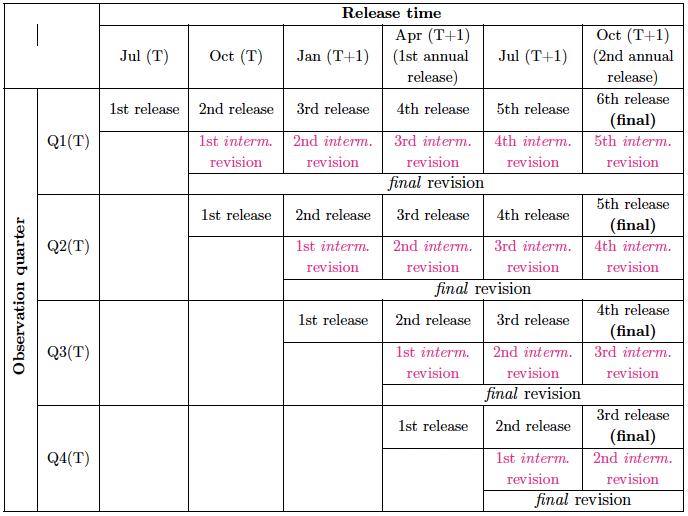
\includegraphics{./rev-chron.png}

}

\caption{\label{fig-rev-chron}Timing of the revisions and underlying
releases}

\end{figure}

To define revisions it is necessary to take a stance which release
constitutes a final value for a certain quarter. Treating the most
recent available observations as final releases may be suboptimal
because of benchmark revisions, which take place every several years and
lead to revisions of not only the most recent quarters but also remote
ones.\footnote{Statistical agencies occasionally adjust their
  methodologies, which leads to revisions of entire time series --- the
  so-called benchmark revisions. In the European Union a harmonised
  European revision policy was put in place to ensure coordinated and
  consistent revisions (see \citet{ec_revision_guidelines}). According
  to this policy, benchmark revisions should take place each five years,
  with implementation years ending with `4' and `9'. Consequently,
  benchmark revisions for ESA 2010, which govern both GFS and MNA, were
  supposed to be implemented in 2014 (at the time of the ESA 2010
  introduction) and 5 years later in 2019. In practice, however, not all
  countries followed the recommendations. Some Member States carried out
  benchmark revisions outside the benchmark years --- before, after or
  even each year including during the benchmark years. The lack of
  regularity makes controlling for benchmark revisions in practice
  extremely challenging.} Against this background, the selection of a
final value becomes a delicate balancing act between two objectives. On
the one hand, there is a desire to incorporate as many releases as
possible to reflect any new incoming information since the moment of the
initial release. On the other hand, one should limit the number of
releases to avoid as much as possible the undesirable contamination of
the dataset with benchmark revisions. The notion of a final value in
this situation becomes necessarily arbitrary. In addition, it should be
recognised that fiscal data even though reported at quarterly frequency
carry some characteristics of annual data, which reflects the annual
nature of budgeting and reporting in the public sector.

In this paper we define the final value for any quarter of year \emph{T}
by the value released in October of the subsequent year \emph{T+1}. The
main motivation for our choice is to duly recognise that quarterly
fiscal data are, at least to some degree, annual in nature. As
documented in Appendix~\ref{sec-Intermediate-revisions}, quarterly
fiscal figures are revised mainly at the time of annual data releases
(i.e.~in April and October). In this context, we regard as final values
the outcomes of the second annual EDP (Excessive deficit procedure)
release.\footnote{As a part of the Excessive deficit procedure all EU
  member states are obliged to report their annual fiscal outturns
  before 1 April and 1 October each year.} At the same time, by keeping
a limited distance between a first and a final release we make the
dataset as much as possible unaffected by benchmark revisions.

The set-up implies that different quarters within a year have a varying
number of releases before the final value is determined (see
Figure~\ref{fig-rev-chron}). Q1 figures require six releases until they
become final while Q4 only three. In other words, while for Q1
observations it takes 1 1/4 years to determine its final values it lasts
only 1/2 year for Q4 observations. The property equally applies to all
variables considered in the analysis therefore it does not affect
comparability between them in any way.

To analyse the revisions we transform the GFS data, expressed in EUR
millions, into growth rates.\footnote{To be precise, we approximate
  growth rates by log differences. The approximation leaves ordinary
  changes over time largely unaffected. However, it diminishes
  extraordinarily huge changes compared to the standard growth rate
  calculation.} In particular, we calculate annual growth rates with
respect to the same quarter of a preceding year. By calculating this
way, rather than with respect to a preceding quarter, we avoid a need
for seasonal adjustment, which in the presence of updates to seasonal
factors would add another source of revisions. Also, considering growth
rates makes the analysis more robust to benchmark revisions than it
would be the case for levels. Benchmark revisions often lead to level
shift adjustments of all quarters, even those reaching far into the
past, but leave the growth profile still largely unaffected. The average
growth for most of the fiscal and macro series in the sample oscillates
around 4\% (see Figure~\ref{fig-mean-standard-deviation-values} in
Appendix~\ref{sec-fiscal-data-characteristics} of the online appendix).

\hypertarget{sec-final_intermediate_revisions}{%
\section{Final and intermediate
revisions}\label{sec-final_intermediate_revisions}}

Final revisions are calculated as a difference between the final release
(\(x_{t}^{f}\)) for quarter \emph{t} and the first release
(\(x_{t}^{1}\)) for the same quarter \(t\) following the below equation:

\[
r_{t}^{f}=x_{t}^{f}-x_{t}^{1}
\]

The definition implies that a positive value is associated with an
underestimation of a first release and the other way around (see the
left-hand-side chart of Figure~\ref{fig-dataoverview1} for
illustration).

Intermediate revisions are calculated as a difference between directly
succeeding data releases as follows:

\[
r_{t}^{i}=x_{t}^{i+1}-x_{t}^{i}
\]

where \(x_{t}^{i}\) is an \emph{i}-th release for quarter \emph{t}.

The sum of intermediate revisions to a given quarterly value amounts to
a final revision (see Figure~\ref{fig-rev-chron} and the right-hand-side
chart of Figure~\ref{fig-dataoverview1} for illustration). In this
context, intermediate revisions can be used to decompose final revisions
--- the aspect we explore in Appendix~\ref{sec-Intermediate-revisions}.
The varying distance between final and initial releases results in a
different number of intermediate revisions depending on a quarter (see
again Figure~\ref{fig-rev-chron} for illustration).

\begin{figure}[H]

{\centering 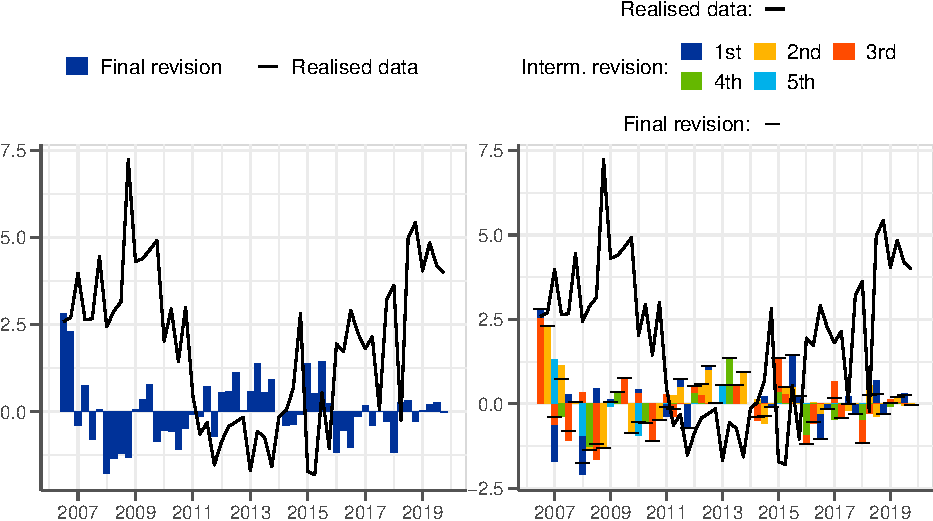
\includegraphics{./2-Data_files/figure-pdf/fig-dataoverview1-1.pdf}

}

\caption{\label{fig-dataoverview1}Revisions to the growth rate of gov.
compensation in the Netherlands}

\end{figure}

\hypertarget{data-scope}{%
\section{Data scope}\label{data-scope}}

Our real-time fiscal dataset contains all main categories provided in
the GFS datasest. We look closely at the following 9 fiscal variables.

\begin{itemize}
\tightlist
\item
  Total revenue

  \begin{itemize}
  \tightlist
  \item
    Direct taxes
  \item
    Indirect taxes
  \item
    Social contributions
  \end{itemize}
\item
  Total expenditure

  \begin{itemize}
  \tightlist
  \item
    Social transfers
  \item
    Purchases
  \item
    Gov.~compensation
  \item
    Gov.~investment
  \end{itemize}
\end{itemize}

The set includes total revenue and total expenditure, as well as their
main components. Table~\ref{tbl-Code-series-fiscal} in the online
appendix gives an overview of all variables together with their full
statistical names and with series keys needed to download the
data.\footnote{Only around 2/3 of the vintages in our real-time fiscal
  dataset are available through ECB's SDW. Vintages published before
  2010 even though public, have not been disseminated to SDW and they
  are based on snapshots of Eurostat data releases.}

We do not explicitly investigate minor fiscal categories, like capital
revenue or subsides, on account of their extraordinary volatility. The
only exception we make is government investment, which belongs to our
particular interests as an important fiscal policy instrument and as a
direct demand component. The excluded variables account only for a
limited share of gov. revenue and expenditure, and as such, they are
usually unable to drive the general picture on fiscal policy.
Concretely, the minor items comprise 10\% of total revenue and 7\% of
total spending in our dataset (see Figure~\ref{fig-ItemShareGDP}). At
the same time, they are very volatile (see standard deviation in
Figure~\ref{fig-mean-standard-deviation-values}) and they come with very
large revisions (see Figure~\ref{fig-revisions_across_variables} and
Figure~\ref{fig-OCR}, Figure~\ref{fig-KTR}, Figure~\ref{fig-INP}, Figure~\ref{fig-OCE}, Figure~\ref{fig-OKE}
in the online appendix). Notwithstanding this, the minor variables are
captured in the analysis by being a part of total revenue and total
expenditure. Consequently, they play a fair role in the analysis even
without being considered individually.

The dataset is supplemented with the selected following items from the
MNA dataset.\footnote{To ensure comparability with fiscal data all
  macroeconomic variables are expressed in nominal terms, therefore they
  also contain the price component.}

\begin{itemize}
\tightlist
\item
  GDP
\item
  Private consumption
\item
  Total investment
\item
  Export
\item
  Gov.~consumption
\item
  Wages and salaries
\end{itemize}

We regard this set of variables as a reliable benchmark for assessing
fiscal revisions. Similarly to the fiscal variables, the series keys
needed for data retrieval are specified in the online appendix in
Table~\ref{tbl-Code-series-macro}.

\begin{figure}[H]

{\centering 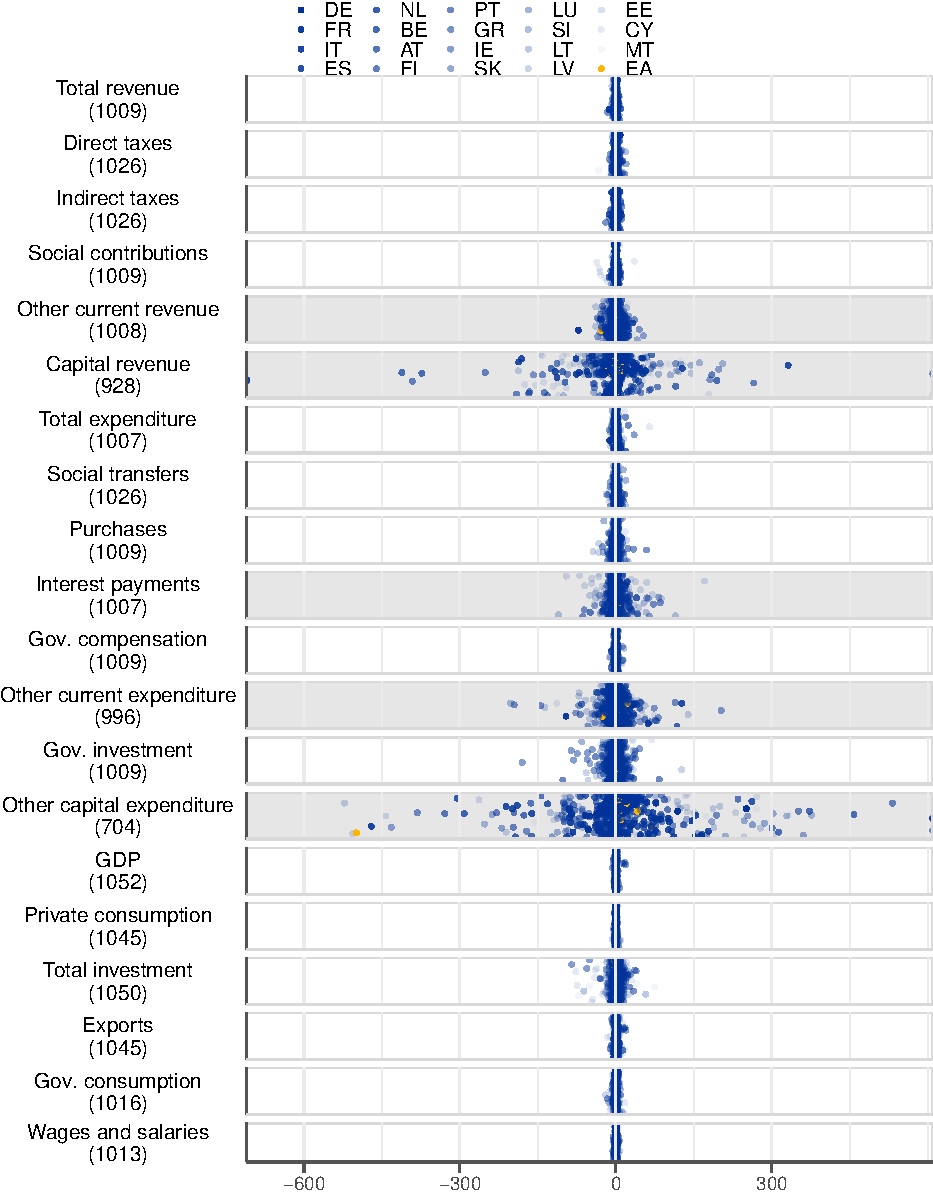
\includegraphics{./2-Data_files/figure-pdf/fig-revisions_across_variables-1.pdf}

}

\caption{\label{fig-revisions_across_variables}Final revisions across
fiscal and macro variables}

\end{figure}

Regarding the country coverage, the dataset underlying the paper
includes all 19 countries comprising currently the EMU, as well as the
euro area aggregate.\footnote{With the intention of saving space the
  following country abbreviations are used throughout the paper: BE
  (Belgium), DE (Germany), EE (Estonia), IE (Ireland), GR (Greece), ES
  (Spain), FR (France), IT (Italy), CY (Cyprus), LV (Latvia), LT
  (Lithuania), LU (Luxembourg), MT (Malta), NL (the Netherlands), AT
  (Austria), PT (Portugal), SI (Slovenia), SK (Slovakia), FI (Finland)
  and EA (the euro area).} For the purpose of our analysis, however, we
consider individually only 9 biggest (in terms government size as
measured by total expenditure) countries. The remaining 10 countries
account for only around 5.5\% of the euro area government expenditure
(see Figure~\ref{fig-share-TOE}) but exhibit extraordinarily high
revisions (see Figure~\ref{fig-revisions_across_countries}). Moreover,
as can be seen in the single-variable revision plots
(Figures~\ref{fig-TOE} - \ref{fig-OCE}, there are instances when fiscal
data for some of these small countries are not subject to any revisions.
Zero revisions in these cases should not support a view about high data
accuracy but rather raise concerns regarding the data quality.

Giving the small and volatile countries a prominent role in forming
conclusions on the euro area fiscal data would be misleading. The
volatility and incompleteness exhibited by these countries does not
influence the big picture on fiscal policy in the euro area simply
because of the small size. For this reason we group the small volatile
10 countries into one geographical unit --- the rest of the euro area
(REA). By doing so we reduce the weight of these countries in the
analysis even though we still cover them. In addition, we occasionally
look at the euro area aggregate, especially with a view to putting the
country fiscal data into perspective.

\begin{figure}[H]

{\centering 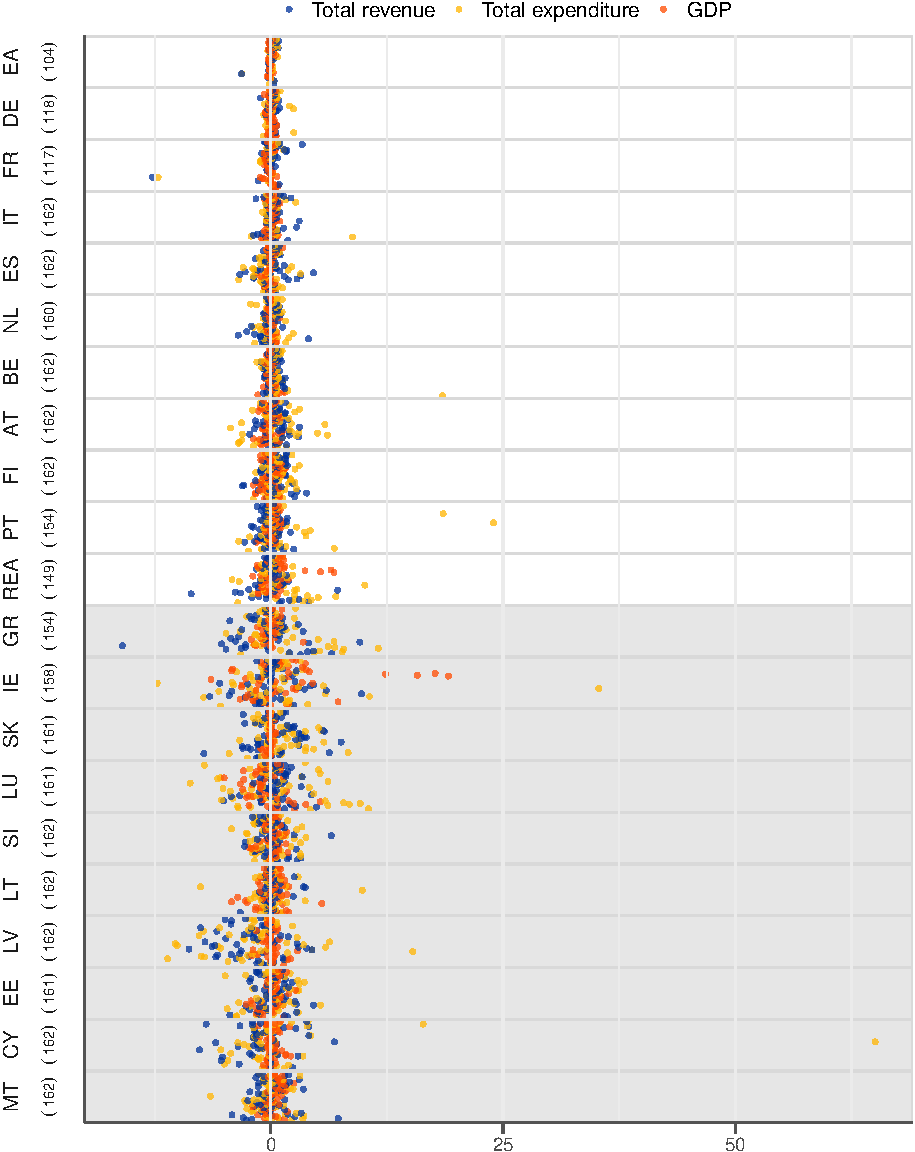
\includegraphics{./2-Data_files/figure-pdf/fig-revisions_across_countries-1.pdf}

}

\caption{\label{fig-revisions_across_countries}Final revisions across
countries}

\end{figure}

Our dataset consists of 59 quarterly GFS vintages taking place since
January 2007 to July 2021. The selection of the first vintage is
dictated by the moment in which quarterly GFS data started being stored
in an organised and complete manner.\footnote{The development work on
  Government Finance Statistics took place since 2002. Only in 2007 the
  data were considered to be of sufficient quality and complete enough
  to be used in economic analysis at the ECB.} Admittedly, it took until
October 2014 before the reporting of the GFS data became compulsory and
complete. Notwithstanding this, even well before October 2014 the GFS
data were published regularly by most of the euro area countries on
voluntary basis.\footnote{Our fiscal real-time dataset contains some
  missing values due to data unavailability before October 2014. Most
  notably, Germany and France published the GFS data only in October
  once per year rather than on quarterly basis.} The last vintage is
simply the release containing final values for 2019, which is the last
year unaffected by the COVID-19 crisis.

\begin{figure}[H]

{\centering 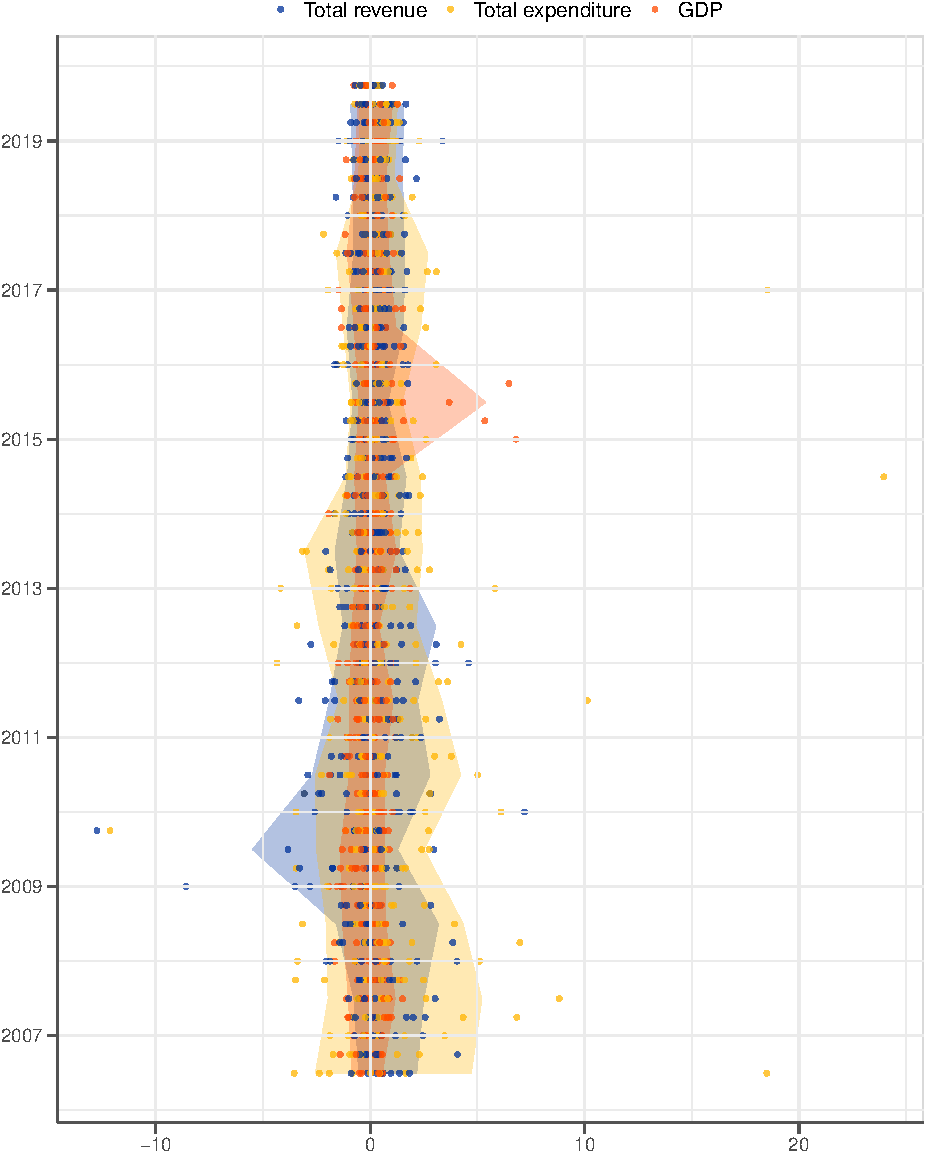
\includegraphics{./2-Data_files/figure-pdf/fig-revisions_over_time-1.pdf}

}

\caption{\label{fig-revisions_over_time}Final revisions across time}

\end{figure}

A look at the data over time reveals that the dispersion of the fiscal
revisions dropped significantly in 2014.
Figure~\ref{fig-revisions_over_time} illustrates that the 5-95\%
interval calculated for each year narrows down noticeably in 2014 for
total revenue and total expenditure. The shrinkage clearly stands out
when the two fiscal variables are compared to GDP. The width of the
interval for the latter stays remarkably constant over the entire period
2007-19 except for 2015 influenced by the extraordinarily high revisions
to Irish GDP. By contrast, the width of the interval for the fiscal
series has been exceeding the one of GDP by a wide margin only until
2014. After 2014, however, the bands of the fiscal series become much
more aligned compared to GDP. The change could be related to the
introduction of ESA 2010 in October 2014 and to the fact that the
reporting of the quarterly fiscal data became compulsory at the time.
While determining the exact reason is outside the scope of our paper we
will bear this fact in mind when analysing the data.

\bookmarksetup{startatroot}

\hypertarget{sec-Magnitude-of-total}{%
\chapter{Unconditional properties of final
revisions}\label{sec-Magnitude-of-total}}

To characterise the revisions we look first at the set of summary
statistics. To this end, we calculate for all fiscal and macro variables
the following metrics:

\begin{itemize}
\tightlist
\item
  Mean revision:
  \(MR=\frac{1}{MT}\sum\limits_{m=1}^{M}\sum\limits_{t=1}^{T}r_{t,m}^{f}\),
  where \emph{m} is a country index, \emph{t} is a time index, \emph{M}
  is the number of countries and \emph{T} is the number of periods
\item
  Maximum and minimum revision: \(MAX=\max{r_{t,m}^{f}}\) and
  \(MIN=\min{r_{t,m}^{f}}\)
\item
  Mean absolute revision:
  \(MAR=\frac{1}{MT}\sum\limits_{m=1}^{M}\sum\limits_{t=1}^{T}|r_{t,m}^{f}\)\textbar{}
\item
  Root mean square revision:
  \(RMSR=\frac{1}{MT}\left[\sum\limits_{m=1}^{M}\sum\limits_{t=1}^{T}\left(r_{t,m}^{f}\right)^{2}\right]^{\frac{1}{2}}\)
\item
  Noise-to-signal ratio (i.e.~the standard deviation of final revisions
  divided by the standard deviations of final values):
  \(N2S=\frac{1}{MT}\left[\sum\limits_{m=1}^{M}\sum\limits_{t=1}^{T}\left(r_{t,m}^{f}-MR\right)^{2}\right]^{\frac{1}{2}}/{\frac{1}{MT}\left[\sum\limits_{m=1}^{M}\sum\limits_{t=1}^{T}\left(x_{t,m}^{f}-\bar{x}_{t}^{f}\right)^{2}\right]^{\frac{1}{2}}}\)
\end{itemize}

The MR statistic will help us assess whether revisions are biased. Other
metrics are useful for assessing the dispersion of the revisions.

\hypertarget{entire-sample-2006q3-2019q4}{%
\section{Entire sample
2006Q3-2019Q4}\label{entire-sample-2006q3-2019q4}}

\begin{figure}[H]

{\centering 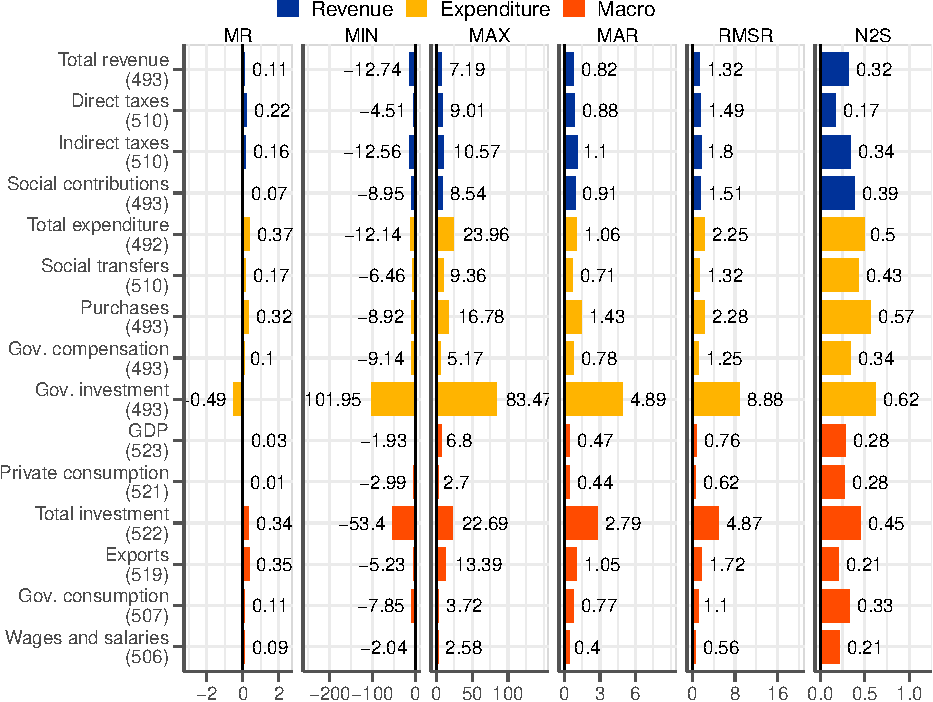
\includegraphics{./3-Uncond-properties_files/figure-pdf/fig-FinRevGItems-1.pdf}

}

\caption{\label{fig-FinRevGItems}Summary statistics of final revisions
in the entire sample}

\end{figure}

The first column of Figure~\ref{fig-FinRevGItems} reports the mean
revision (MR), which is informative about the bias. The results point to
a positive MR for all fiscal variables except for government investment.
The interpretation of these results is that statistical agencies tend to
initially underestimate fiscal figures. Regarding the size, MR for most
of the variable falls into the interval of 0.1-0.3 percentage points.
Given that the average growth rate for most of the variables in the
sample is slightly above 4\% (see
Figure~\ref{fig-mean-standard-deviation-values}) the revision bias is
non-negligible, albeit not large. While GDP and private consumption
appear to be unbiased other macro variables have a positive MR, like the
fiscal variables.

The next two columns present the MIN-MAX range of revisions. The
intervals are relatively wide, and in some cases extremely wide (see,
for instance, government investment with the range from \(-102\) to
\(+83\) percentage points). Even the fiscal variables with the most
contained ranges, like social transfers, are associated with a wider
interval than the usually stable macro categories (i.e. output, private
consumption or wages and salaries). The MIN-MAX interval is a first
indication that the revisions to fiscal variables may be larger than
these associated with the macro data.

Next we report the mean absolute revision (MAR), which by contrast to
MR, ensures that negative and positive revisions do not cancel each
other out. The statistic summarises the magnitude of the revisions by
treating all of them, regardless their sign and size, equally. It turns
out that the least revised fiscal items are variables on the revenue
side as well as big categories on the spending side, namely social
transfers and gov. compensation. MAR associated with them tends to
remain below 1 percentage point. The values are significantly higher
than for MR and should be regarded as relatively sizeable given the
average growth of these variables in the sample (around 4\%). MAR values
for these fiscal variables are approximately double of the corresponding
statistics for the stable macroeconomic variables (i.e.~output, private
consumption and wages and salaries) amounting to around 0.5 percentage
points, which are by no means small. MAR statistics for the remaining
fiscal variables are even higher with government investment being
characterised by the largest figure (almost 5 percentage points, which
even exceeds the average growth rate of this variable below 4\%, as can
be seen in Figure~\ref{fig-mean-standard-deviation-values}).

The fifth column of Figure~\ref{fig-FinRevGItems} reports the
root-mean-square revision (RMSR). Compared to MAR, this statistics
penalises big revisions by means of squaring. Notwithstanding this, RMSR
gives broadly the same picture as MAR. Its contribution is a
magnification of the metric for variables that are subject to big
revisions, like government investment, which stands out even by a wider
margin than in the case of MAR.

Finally, in the last column we report the noise-to-signal ratio (N2S),
which compared to RMSR takes into account the volatility of a variable
itself. This measure brings the fiscal variables closer to the macro
variables. Since fiscal categories tend to be more volatile compared to
the macro variables (see
Figure~\ref{fig-mean-standard-deviation-values}) it is natural that they
are more heavily revised. The N2S statistic reflects upon this
consideration. Judging by this measure direct taxes turn out to be the
variable with the smallest relative revisions. Moreover, the heavily
revised government investment do not appear so exceptional any longer
compared to other variables.

To sum up the results of Figure~\ref{fig-FinRevGItems}, it turns out
that almost all variables we consider in the analysis are associated
with a positive bias, as judged by the MR statistic. The notable
exceptions are output and private consumption, which both have roughly a
zero mean, and government investment, which has a negative mean. Other
measures, namely MIN-MAX range, MAR and RMSR, indicate that the
revisions tend to have large dispersion. This particularly applies to
fiscal variables, which record twice as large MAR compared to macro
variables (at least when it comes to the most stable and largest
categories in the two groups). Moreover, government investment, clearly
stands out as particularly sensitive to big revisions, similarly to
total investment. Once we recognise the fact that certain variables tend
to be more volatile than others the variation across variables
diminishes considerably, as captured by the N2S ratio statistic.

\hypertarget{pre-and-post-2014q2-subsamples}{%
\section{Pre and post-2014Q2
subsamples}\label{pre-and-post-2014q2-subsamples}}

The analysis presented above indicated that fiscal revisions exhibit
considerably bigger dispersion than macro revisions (i.e.~approximately
twice as big when measured by MAR). This is in line with the existing
literature, which states that fiscal variables are subject to
particularly sizeable revisions (see, for instance,
\citet{Cimadomo_2016_jes}). This widely held view casts severe doubts on
the quality of fiscal data in real time. Having in mind the illustration
in Figure~\ref{fig-revisions_over_time} indicating that fiscal revisions
in the euro area dropped significantly over time we re-evaluate the
existing belief. To this end, we split the sample in 2014Q2, which is
the quarter for which the initial release was reported according to ESA
2010 for the first time. Also, 2014 is the point at which the reporting
of Government Finance Statistics became obligatory, even though
countries had been reporting them on voluntary basis before. Having
split the sample, coincidentally into two roughly equal parts, we
recalculate the summary statistics for the two subsamples.

\begin{figure}

\begin{minipage}[t]{\linewidth}

{\centering 

\raisebox{-\height}{

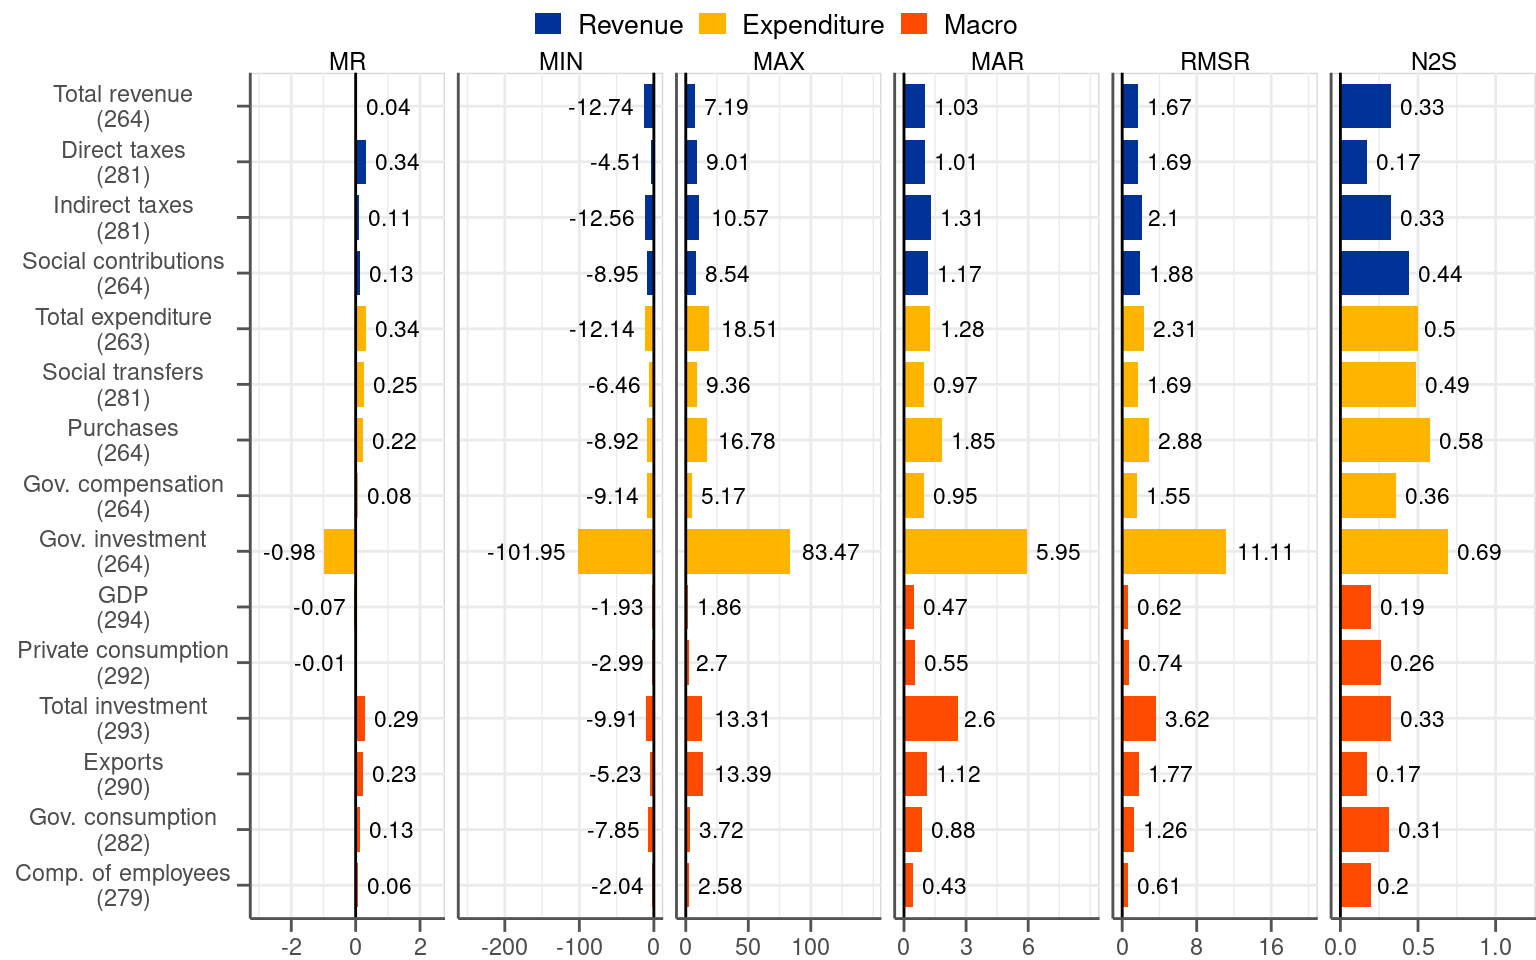
\includegraphics{./3-Uncond-properties_files/figure-pdf/fig-RevGItems_prepost2014-1.pdf}

}

}

\subcaption{\label{fig-RevGItems_prepost2014-1}pre-2014Q2}
\end{minipage}%
\newline
\begin{minipage}[t]{\linewidth}

{\centering 

\raisebox{-\height}{

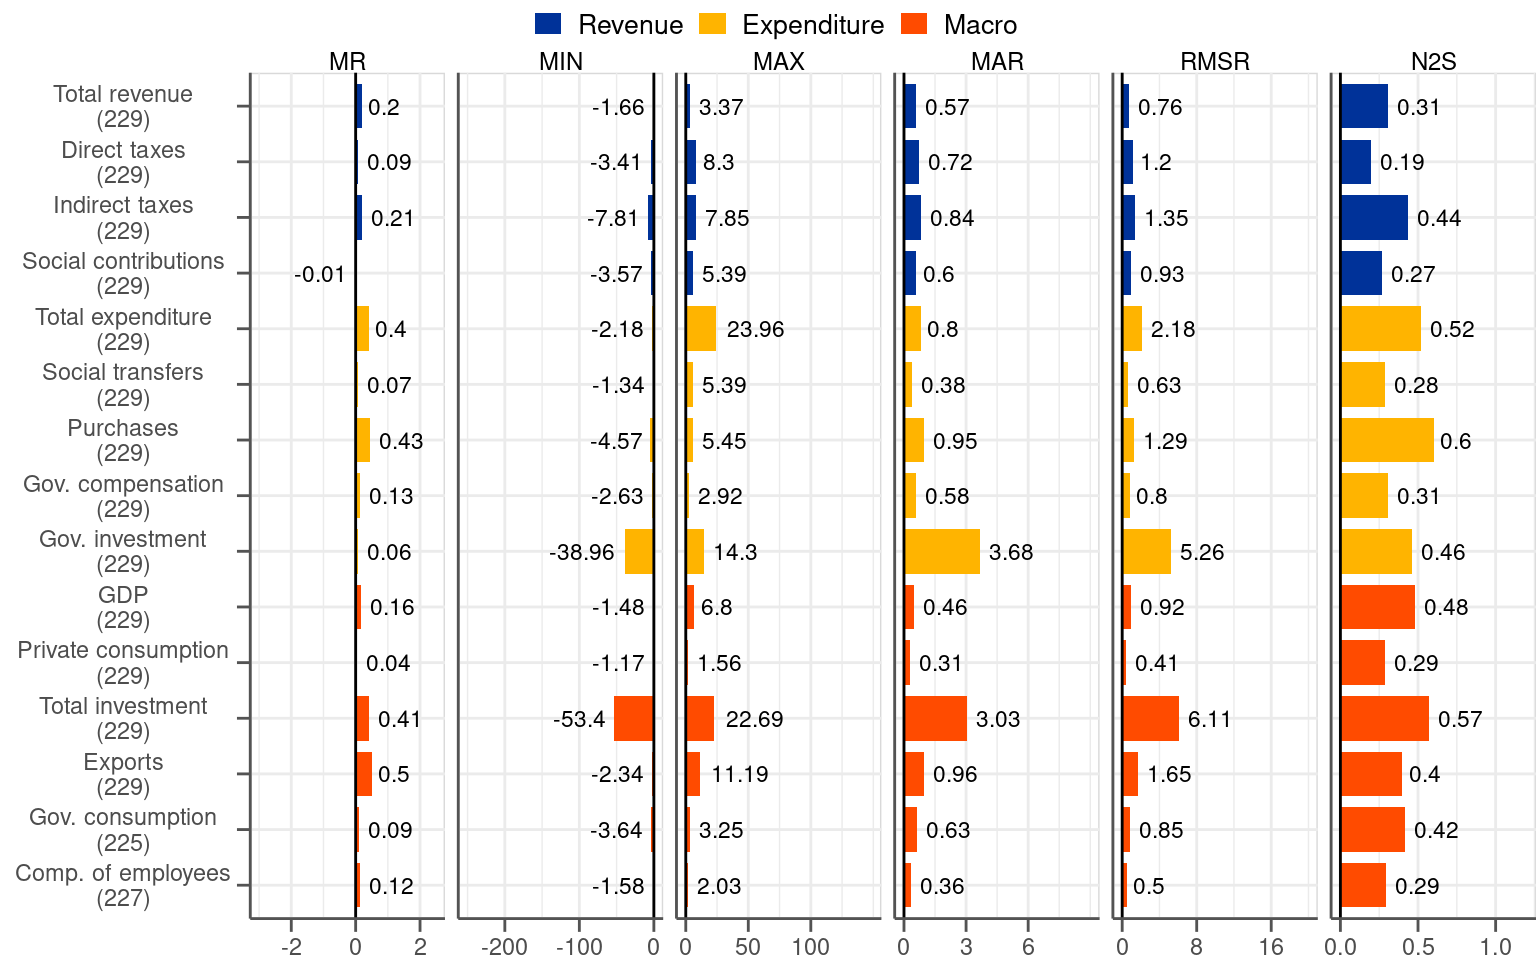
\includegraphics{./3-Uncond-properties_files/figure-pdf/fig-RevGItems_prepost2014-2.pdf}

}

}

\subcaption{\label{fig-RevGItems_prepost2014-2}post-2014Q2}
\end{minipage}%

\caption{\label{fig-RevGItems_prepost2014}Summary statistics of final
revisions in the two subsamples}

\end{figure}

A close look at Figure~\ref{fig-RevGItems_prepost2014} reveals that
summary statistics in the two periods differ considerably for fiscal
variables. While the MR metric points to a positive bias of a comparable
magnitude in the both subsamples the differences for statistics
representing dispersion are stark. Just to start with, the MIN-MAX
interval reported in the second and third column of
Figure~\ref{fig-RevGItems_prepost2014} shrinks significantly for fiscal
variables in the post 2014Q2 subsample. In the same vein, the variables
in the second subsample are associated with considerably lower
(i.e.~around half for most of the items) MAR compared to the first
subsample. As easy to anticipate, the same applies to the RMSR measure.

No similar reduction in the statistics measuring the dispersion of the
revisions is visible for the macro variables. The MAR statistic, which
we regard as the most illustrative, remains broadly the same between the
two subsamples. Even though the values differ slightly, no systematic
reduction in the metric is visible in the post-2014Q2 subsample.

In general and as expected, the summary measures point out a
considerable drop in the magnitude of fiscal revisions in October 2014.
The second subsample, which captures post-ESA 2010 introduction
observations, is more representative for the description of the current
features of the data rather than the entire sample, let alone the first
subsample under ESA 95. Looking at Figure~\ref{fig-FinRevGItems} and
Figure~\ref{fig-RevGItems_prepost2014} it becomes evident that the
statistics for the entire sample are heavily affected by the
extraordinarily high values present in the first subsample.\footnote{Some
  extraordinary values of the revisions in the first subsample may
  relate to the Great Financial Crisis. At the time governments
  undertook multiple support measures, most notably to assist the
  financial sector. The statistical recording of the associated
  transactions was more uncertain than usually.} If the objective of the
analysis is to characterise the current properties of the revisions more
focus should be given to the post-2014Q2 horizon.

As fiscal revisions drop significantly in size and macro revisions
remain broadly unchanged the difference between the two types of
variables narrows down by a considerable margin. Concretely, post-2014Q2
MAR for fiscal variables is in the same ballpark as for macro
categories. The MAR measure does not exceed significantly 0.5 percentage
points in the case of both types of variables.

All in all, our analysis contradicts the claim that fiscal variables are
particularly prone to revisions. Since 2014 the degree to which fiscal
variables are revised is not considerably different compared to macro
variables. This is not to say that the revisions are well-behaved as the
opposite comes out of our analysis. In the second subsample, which is
more representative for describing current data properties, the
revisions to both fiscal and macro variables are positively biased and
still dispersed. The two properties stand in contrast with the
requirements for well-behaved revisions.

\bookmarksetup{startatroot}

\hypertarget{sec-Intermediate-revisions}{%
\chapter{Properties of intermediate
revisions}\label{sec-Intermediate-revisions}}

Intermediate revisions are changes that take place between subsequent
releases, as explained in
Subsection~\ref{sec-final_intermediate_revisions}. By construction,
intermediate revisions make up for final revisions (as illustrated in
Figure~\ref{fig-dataoverview1}). Analysing intermediate revisions is
indispensable for understanding the dynamics between initial and final
releases. As such, intermediate revisions can foster understanding of
final revisions.

Intuitively, each release should bring the data closer to its final
value as gradually with time more information becomes available to data
compilers (see the right-hand-side chart in
Figure~\ref{fig-dataoverview1} where most of the intermediate revisions
go in the direction of the final revisions). In practice, however, it
occurs that some releases go into the opposite direction and increase
the distance to the final value compared to a previous release.
Figure~\ref{fig-single_rev_example} provides an example of a data point
where the initial release was closer to the final value than subsequent
releases (see the case of Austria). If such cases are frequent our
findings based on final revisions may considerably change (as
demonstrated with a single calculation on
Figure~\ref{fig-single_rev_example}), which we verify in this
section.\footnote{If all intermediate revisions went towards a final
  value (i.e.~are of the same sign as a final revision) intermediate
  revisions would not bring any additional information to the summary
  statistics calculated based on final revisions. MAR, for instance,
  would be just lower by a certain factor because final revisions could
  be divided into smaller pieces constituting intermediate revisions.}

\begin{figure}[H]

{\centering 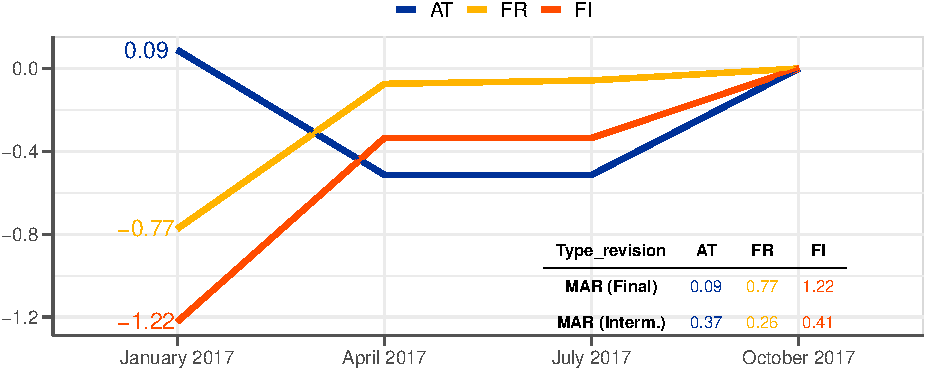
\includegraphics{./5-Intermediate-revisions_files/figure-pdf/fig-single_rev_example-1.pdf}

}

\caption{\label{fig-single_rev_example}Revisions to the growth rate of
2016Q3 social contributions}

\end{figure}

Another aspect that can be revealed by analysis of intermediate
revisions is the timing of the revisions. In this context, the analysis
should inform us whether the revisions mostly take place shortly after
an initial release or maybe closer to the publication of a final value.
In the same vein, it will be possible to identify releases within a year
(i.e.~Jan, Apr, Jul or Oct) when the data are subject to particular
revisions, if this is the case.

\hypertarget{unconditional-properties}{%
\section{Unconditional properties}\label{unconditional-properties}}

Figure~\ref{fig-inRevGItems_prepost2014} contains summary statistics of
intermediate revisions. Given the great relevance of the 2014Q2 split
and its profound effects on the reduction in fiscal revisions, as
discussed in Appendix~\ref{sec-Magnitude-of-total}, we present directly
the results in the two subsamples. Similarly to
Figure~\ref{fig-RevGItems_prepost2014} for final revisions, we report a
set of summary statistics.

The picture constructed on the basis of intermediate revisions is very
similar to the one based on final revisions. On the bias, intermediate
revisions do not bring any new information to the MR statistic compared
to final revisions. The value of the metric is just lower by a constant
factor compared to the one based on final revisions. This is not
surprising because the change from the initial release to the final
release is captured in multiple intermediate revisions rather than in
one final revision. Since final revisions consist of 2, 3, 4 or 5
intermediate revisions depending on a quarter there are around 3.5
intermediate revisions per one final revision on average. This is
exactly the factor by which the MR statistics based on intermediate
revisions is lower compared to the one based on final
revisions.\footnote{The factor can deviate slightly due to missing
  observations.}

Regarding the dispersion of intermediate revisions, even though they
bring new information they paint a very similar picture compared to
final revisions. The value of the MAR statistics, which we consider to
be the most illustrative as a measure of dispersion, is lower compared
to the final revisions. The ratio between the two is not roughly 3.5 but
significantly less (i.e.~slightly above 2 on average for most of the
variables). This indicates that releases that bring data away from final
values are relatively common in the dataset.

Notwithstanding these undesirable releases, intermediate revisions point
to the same conclusions on the dispersion of the revisions like the
final ones. In the pre-2014Q2 subsample fiscal revisions are
approximately twice as dispersed as macro revisions, as judged by the
MAR measure for the biggest and most stable categories. In the
post-2014Q2 subsample the MAR measure for both types of variables fiscal
and macro are not far away from each other. Volatile categories, in
particular government and total investment, are associated with
exceptionally high values of the statistics measuring dispersion,
especially in the second subsample.

\begin{figure}

\begin{minipage}[t]{\linewidth}

{\centering 

\raisebox{-\height}{

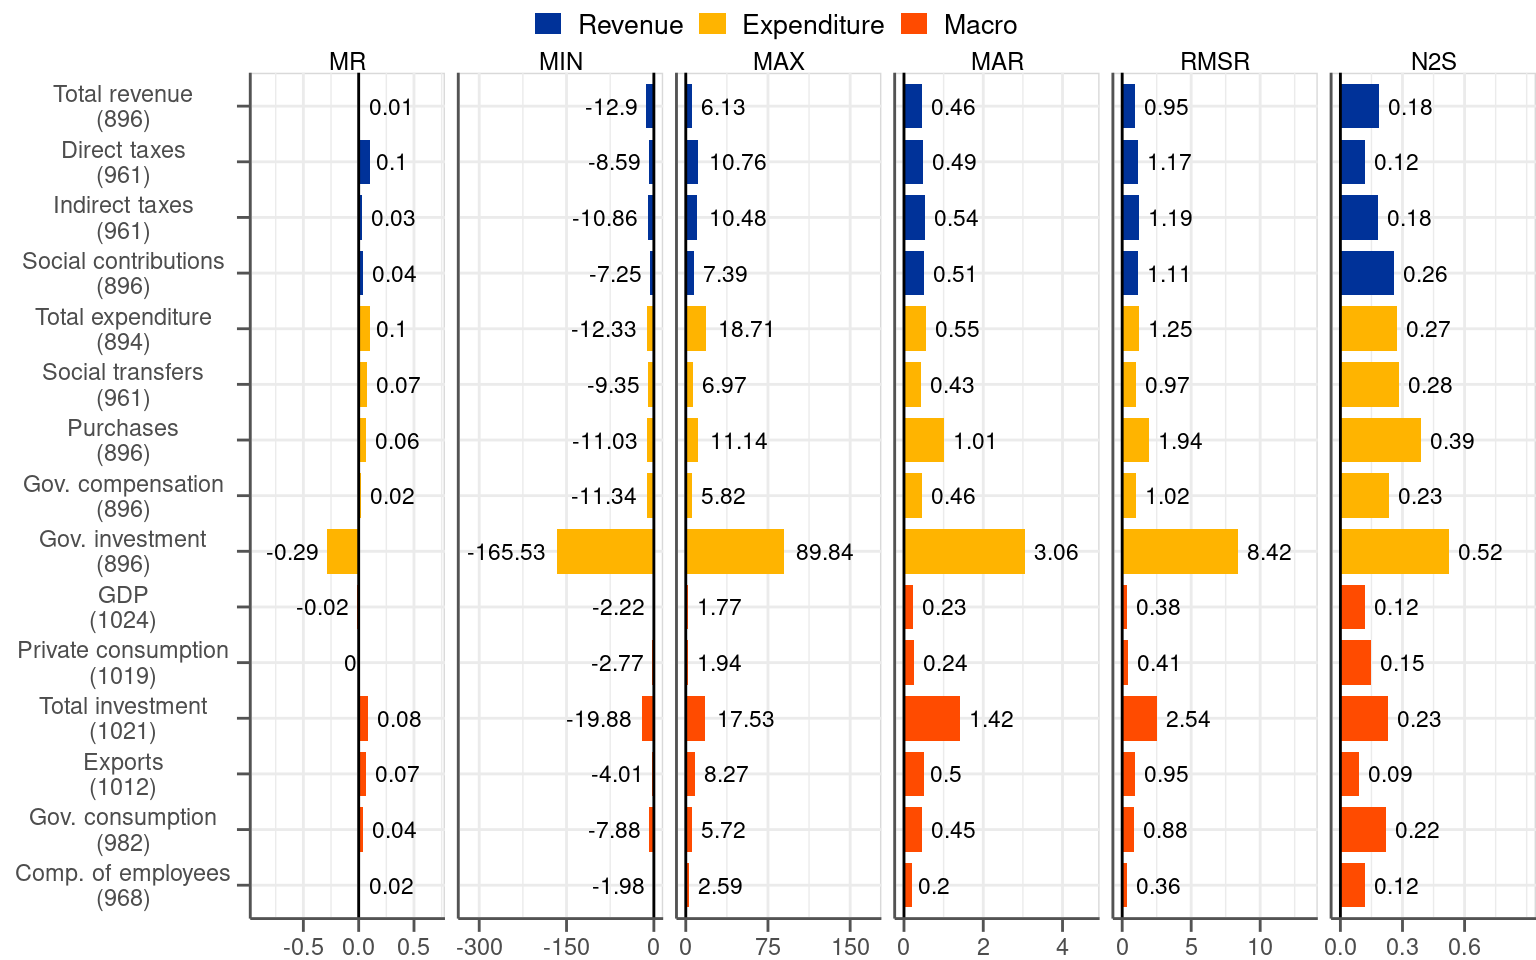
\includegraphics{./5-Intermediate-revisions_files/figure-pdf/fig-inRevGItems_prepost2014-1.pdf}

}

}

\subcaption{\label{fig-inRevGItems_prepost2014-1}pre-2014Q2}
\end{minipage}%
\newline
\begin{minipage}[t]{\linewidth}

{\centering 

\raisebox{-\height}{

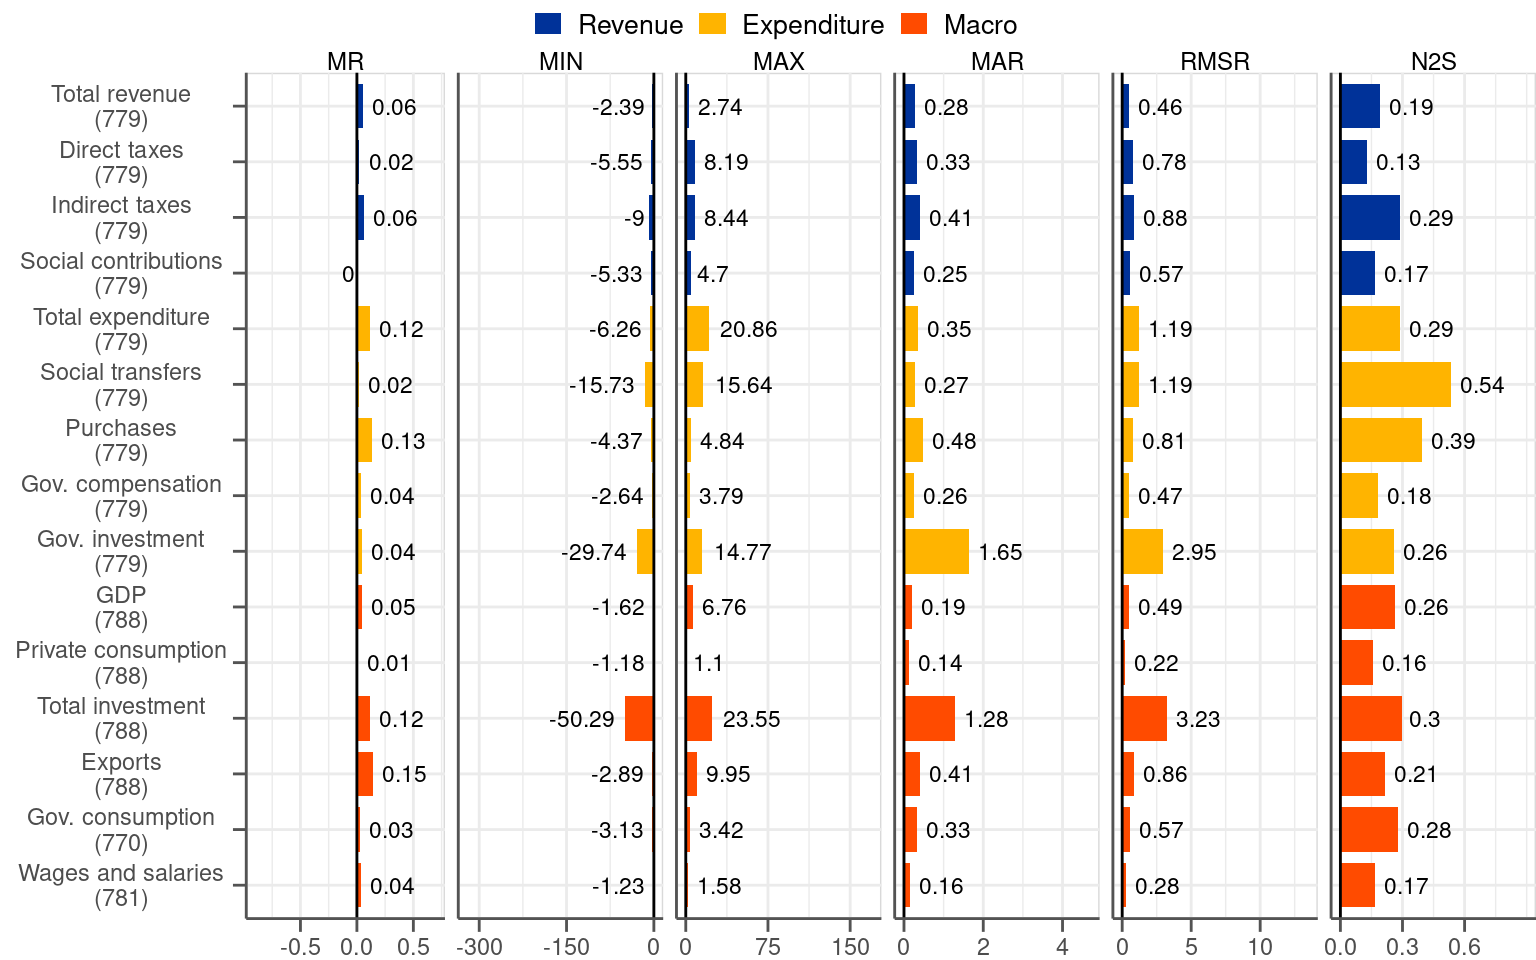
\includegraphics{./5-Intermediate-revisions_files/figure-pdf/fig-inRevGItems_prepost2014-2.pdf}

}

}

\subcaption{\label{fig-inRevGItems_prepost2014-2}post-2014Q2}
\end{minipage}%

\caption{\label{fig-inRevGItems_prepost2014}Summary statistics of
intermediate revisions in the two subsamples}

\end{figure}

\hypertarget{sec-revisions_timing}{%
\section{Dynamics of data releases}\label{sec-revisions_timing}}

Another aspect on which intermediate revisions can shed light is the
evolution of releases from the initial one to the final one. This will
inform us about the path that intermediate data releases undertake when
they converge to the final value. Such analysis should also confirm one
of the findings from the previous subsection, namely the existence of
incidents when intermediate releases take data away from final values
compared to figures already published. Given that the number of
intermediate revisions differs depending on a quarter (i.e.~Q1
observations have 5 intermediate revisions while Q4 observations only 2
intermediate revisions) we look at Q1-Q4 observations separately (see
Figure~\ref{fig-Single_Rev_Path}).

Figure~\ref{fig-Single_Rev_Path} illustrates how initial releases
converge towards final values. Strictly speaking, the lines in the
charts demonstrate how final revisions, associated with initial
releases, move during the revision cycle towards zero, which is the
moment of final release. Each line represents average revisions for one
variable. Since the conclusions we draw below remain valid for both pre
and post-2014Q2 subsamples (see \textbf{?@fig-Single-Rev-Path-pre2014}
and \textbf{?@fig-Single-Rev-Path-post2014} for the two subsamples in
the online appendix). Figure~\ref{fig-Single_Rev_Path} is based on the
dataset without the split.

Looking at the shapes of the lines in Figure~\ref{fig-Single_Rev_Path}
it becomes clear that the evolution of revisions, which bring data to
final values, is different for fiscal and macro variables. For the
former the most sizable data revisions take place in April and in
October of the following year (see that the lines leading to Apr T+1 and
Oct T+1 are the steepest of all fragments). These are the releases
coinciding with EDP notifications. In April T+1 data for Q4 of year T
and for the year as a whole become published for the first time. October
T+1 is the second EDP notification for year T when all its quarters can
be subject to changes. The release of October T+1 also defines final
values in our analysis.\footnote{As emphasised in
  \citet{MaurerKeweloh2017_ecb-sps} also EDP Dialogue visits have
  measurable impact on deficit revisions. To the extent that they have
  an impact on EDP Notifications they exacerbate revisions in April and
  October.} By contrast, the revisions for macro variables occur much
more gradually (see that the lines are less of a step-wise profile)
compared to fiscal variables. This shows that macro variables are
revised irrespective of the quarter. January and July releases are also
associated with sizable revisions, which is not the case for fiscal
variables.

Even by looking at the aggregated data single instances of lines
trending upwards are visible (see Figure~\ref{fig-Single_Rev_Path}).
This only re-affirms that cases where single releases takes us away from
final values compared to a preceding release exist in the dataset.
Naturally, in such cases the subsequent revisions need to be
particularly large as they need to make up for any move in the `wrong'
direction.

\begin{figure}[H]

{\centering 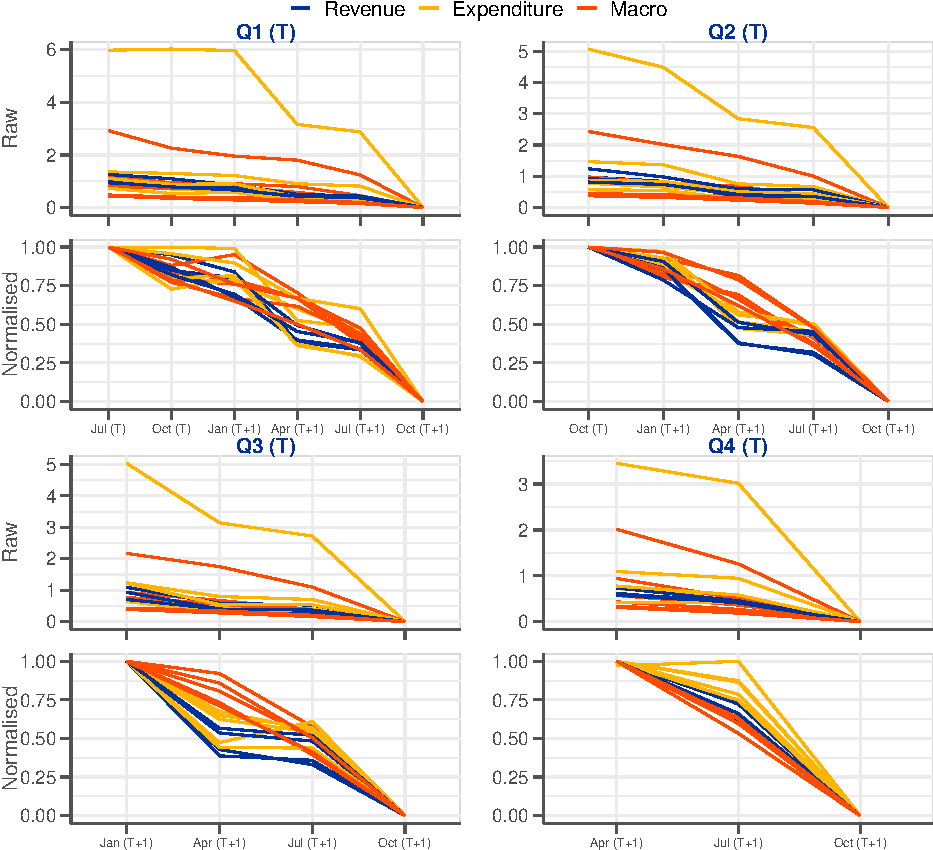
\includegraphics{./5-Intermediate-revisions_files/figure-pdf/fig-Single_Rev_Path-1.pdf}

}

\caption{\label{fig-Single_Rev_Path}Revision paths across variables}

\end{figure}

\bookmarksetup{startatroot}

\hypertarget{sec-Conclusions}{%
\chapter{Conclusions}\label{sec-Conclusions}}

Our investigation concludes that fiscal revisions are badly-behaved.
They fulfil none of the requirements for well-behaved revisions. More
specifically, (1) fiscal revisions exhibit a positive bias, (2) they are
characterised by a considerable dispersion and (3) they are in general
predictable with the information available at the time of the initial
release.

While our analysis concludes that fiscal revisions are badly-behaved it
is difficult to find support in the data that they are worse than macro
revisions presently. Macro revisions are also badly-behaved, which has
been already documented in the literature (see, e.g.,
\citet{Faust2005NewsAN}). The extent of this `misbehaviour' is just
similar for the two types of variables. Both macro and fiscal revisions
exhibit similar bias and they are subject to a comparable dispersion,
most notably since 2014 when fiscal revisions became more contained.
Moreover, no major difference emerges in the analysis between the two
types of revisions when it comes to predictability.

Supplementing the analysis with the intermediate revisions leaves the
conclusions unchanged. Notwithstanding this, intermediate revisions do
bring additional information to the study. Most notably, they make clear
that fiscal variables converge to final values differently from macro
variables. While for the former the revisions tend to take place in
April and October a more evenly distributed revision pattern is observed
for the latter.

\bookmarksetup{startatroot}

\hypertarget{references}{%
\chapter*{References}\label{references}}
\addcontentsline{toc}{chapter}{References}

\markboth{References}{References}

\hypertarget{refs}{}
\begin{CSLReferences}{0}{0}
\end{CSLReferences}

\cleardoublepage
\phantomsection
\addcontentsline{toc}{part}{Appendices}
\appendix

\hypertarget{sec-Revisions-illustration}{%
\chapter{Graphical illustration of the
revisions}\label{sec-Revisions-illustration}}

All final revisions to variables considered (but not necessarily
included) in the analysis are illustrated in this appendix section with
the twofold objective. First, the graphs are useful for illustrating the
magnitude of the revisions across variables and countries. Second, the
plots are indispensable to potentially identify any issues with the
dataset that could impair our analysis (e.g.~excessive values or lack of
revisions). Appendix~\ref{sec-code-retrieval} of the online appendix
provides statistical codes used to retrieve the data.

\hypertarget{fiscal-revenue-variables}{%
\section{Fiscal revenue variables}\label{fiscal-revenue-variables}}

\begin{figure}[H]

{\centering 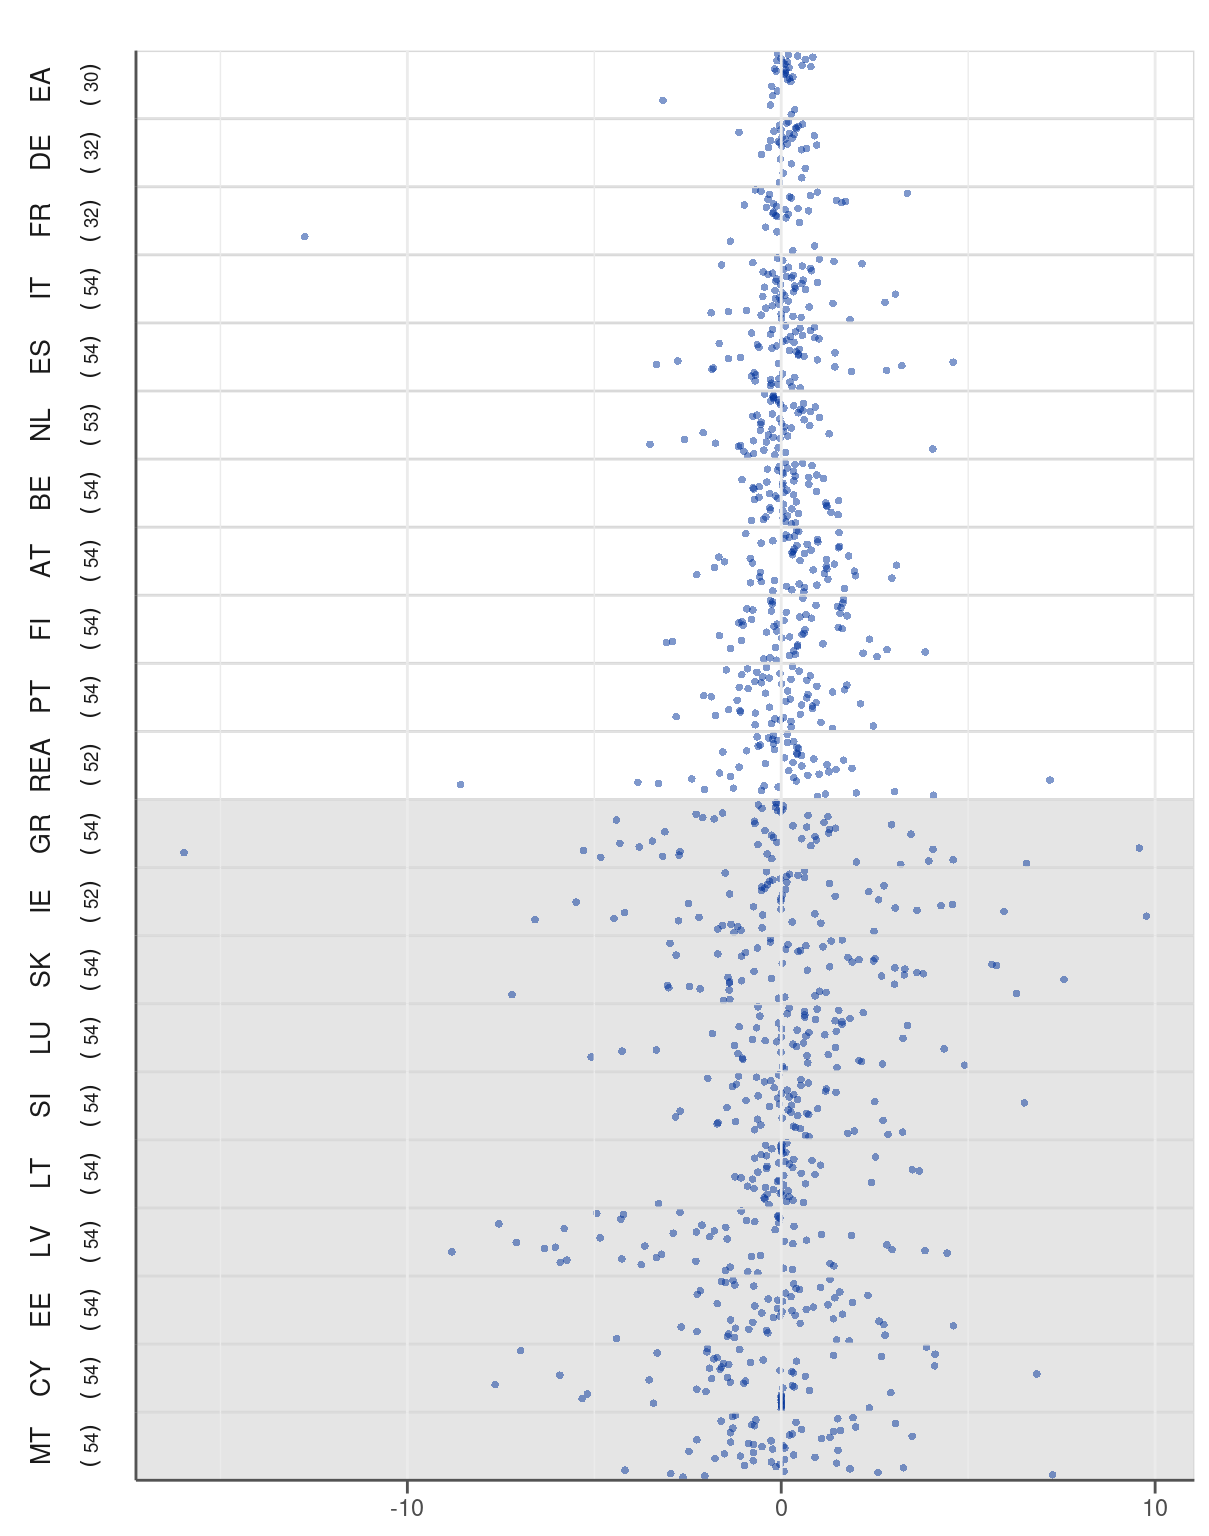
\includegraphics{./A-Graphs-revisions_files/figure-pdf/fig-TOR-1.pdf}

}

\caption{\label{fig-TOR}Final revisions to total revenue}

\end{figure}

\pagebreak

\begin{figure}[H]

{\centering 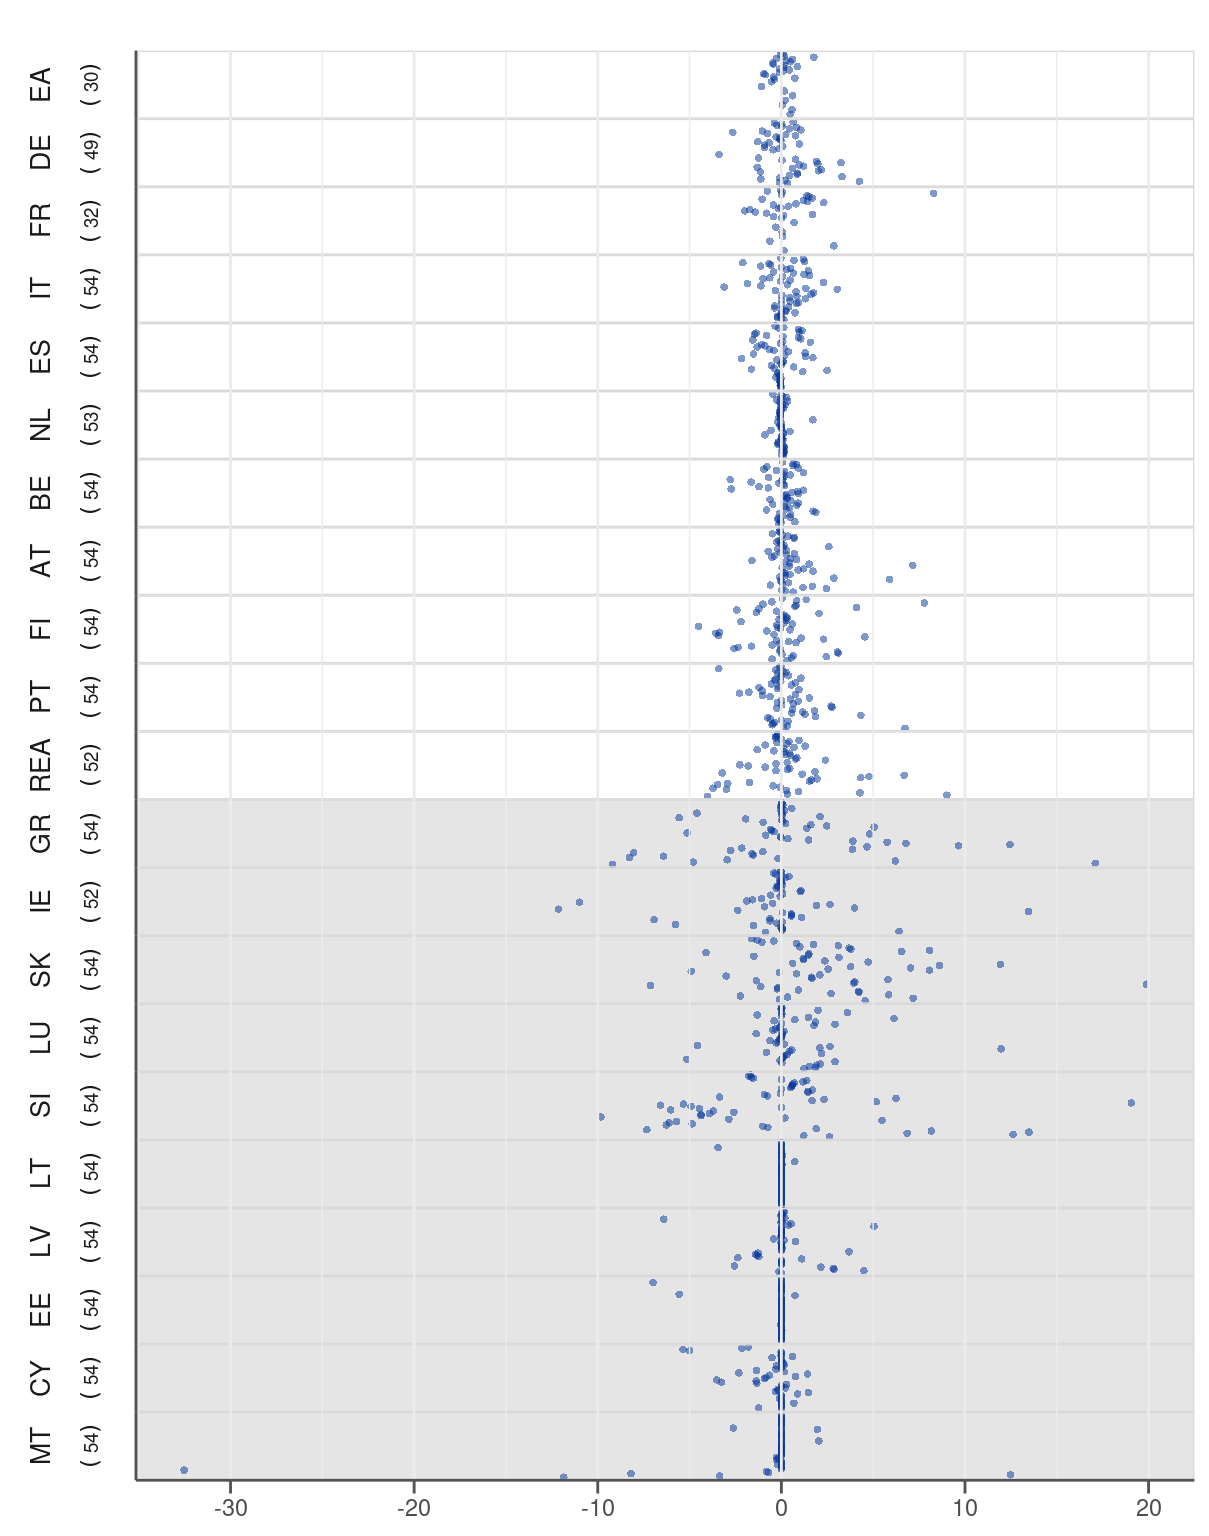
\includegraphics{./A-Graphs-revisions_files/figure-pdf/fig-DTX-1.pdf}

}

\caption{\label{fig-DTX}Final revisions to direct taxes}

\end{figure}

\pagebreak

\begin{figure}[H]

{\centering 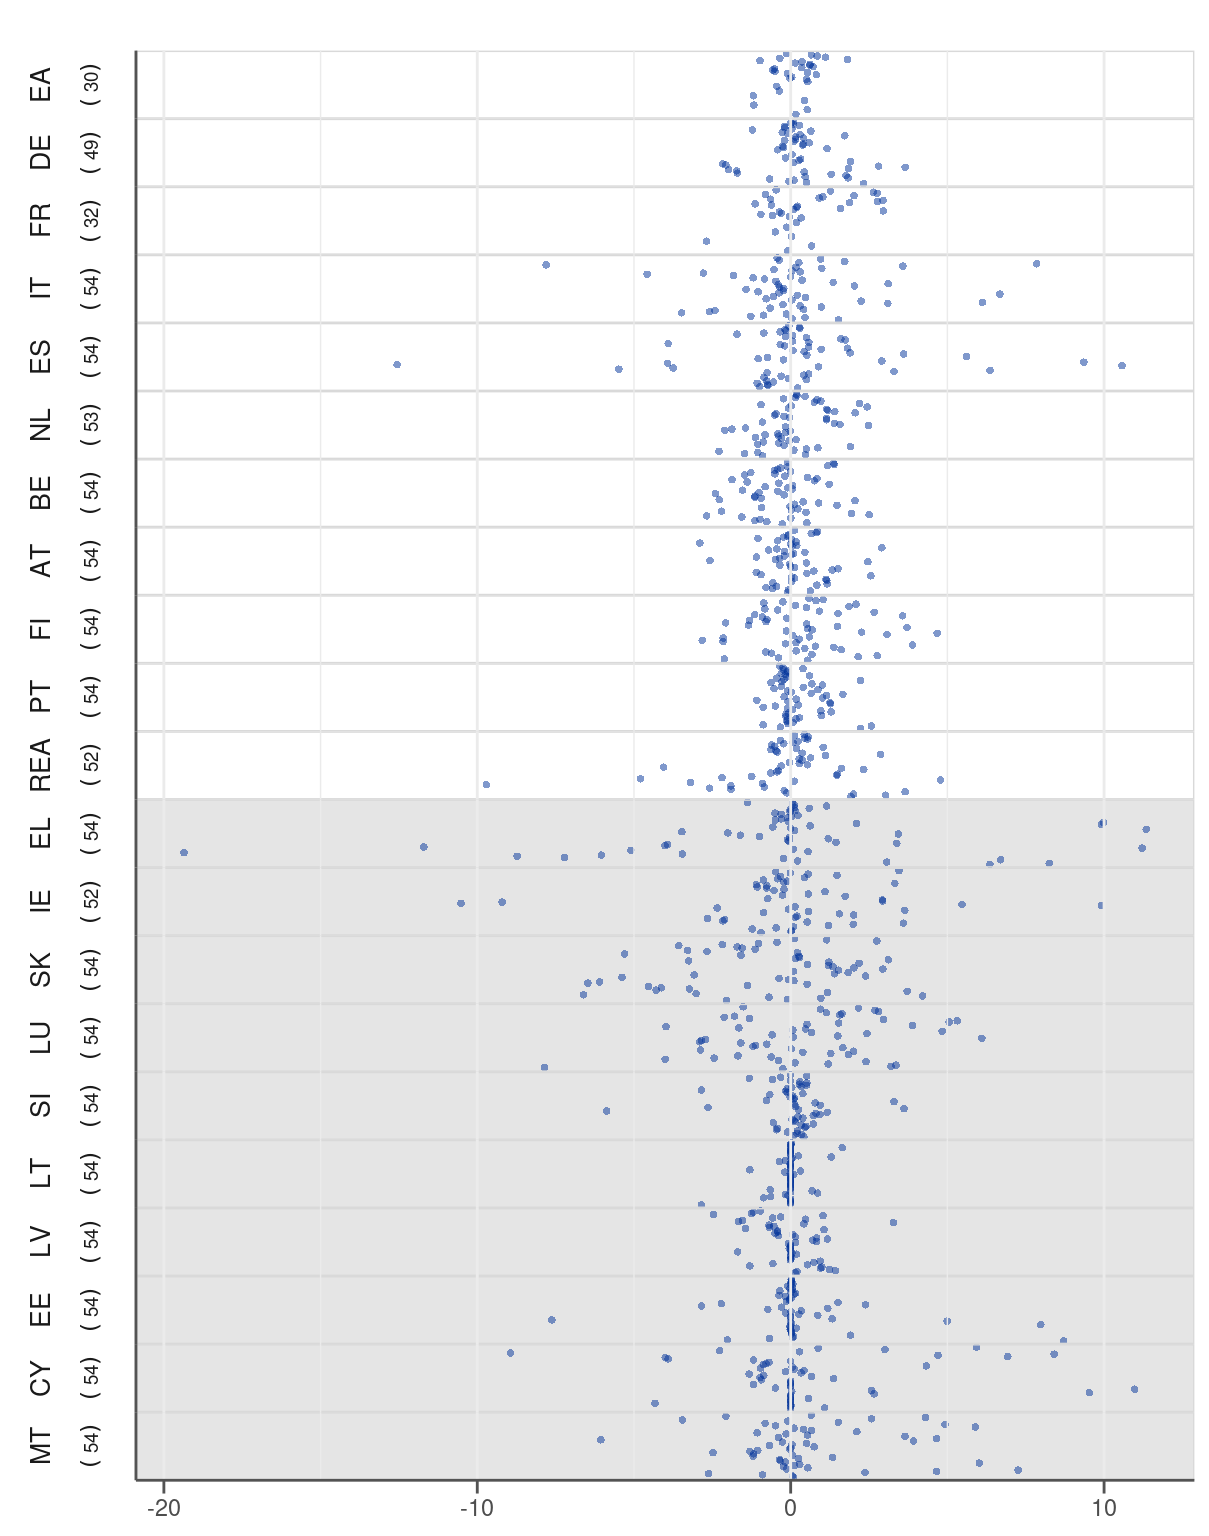
\includegraphics{./A-Graphs-revisions_files/figure-pdf/fig-TIN-1.pdf}

}

\caption{\label{fig-TIN}Final revisions to indirect taxes}

\end{figure}

\pagebreak

\begin{figure}[H]

{\centering 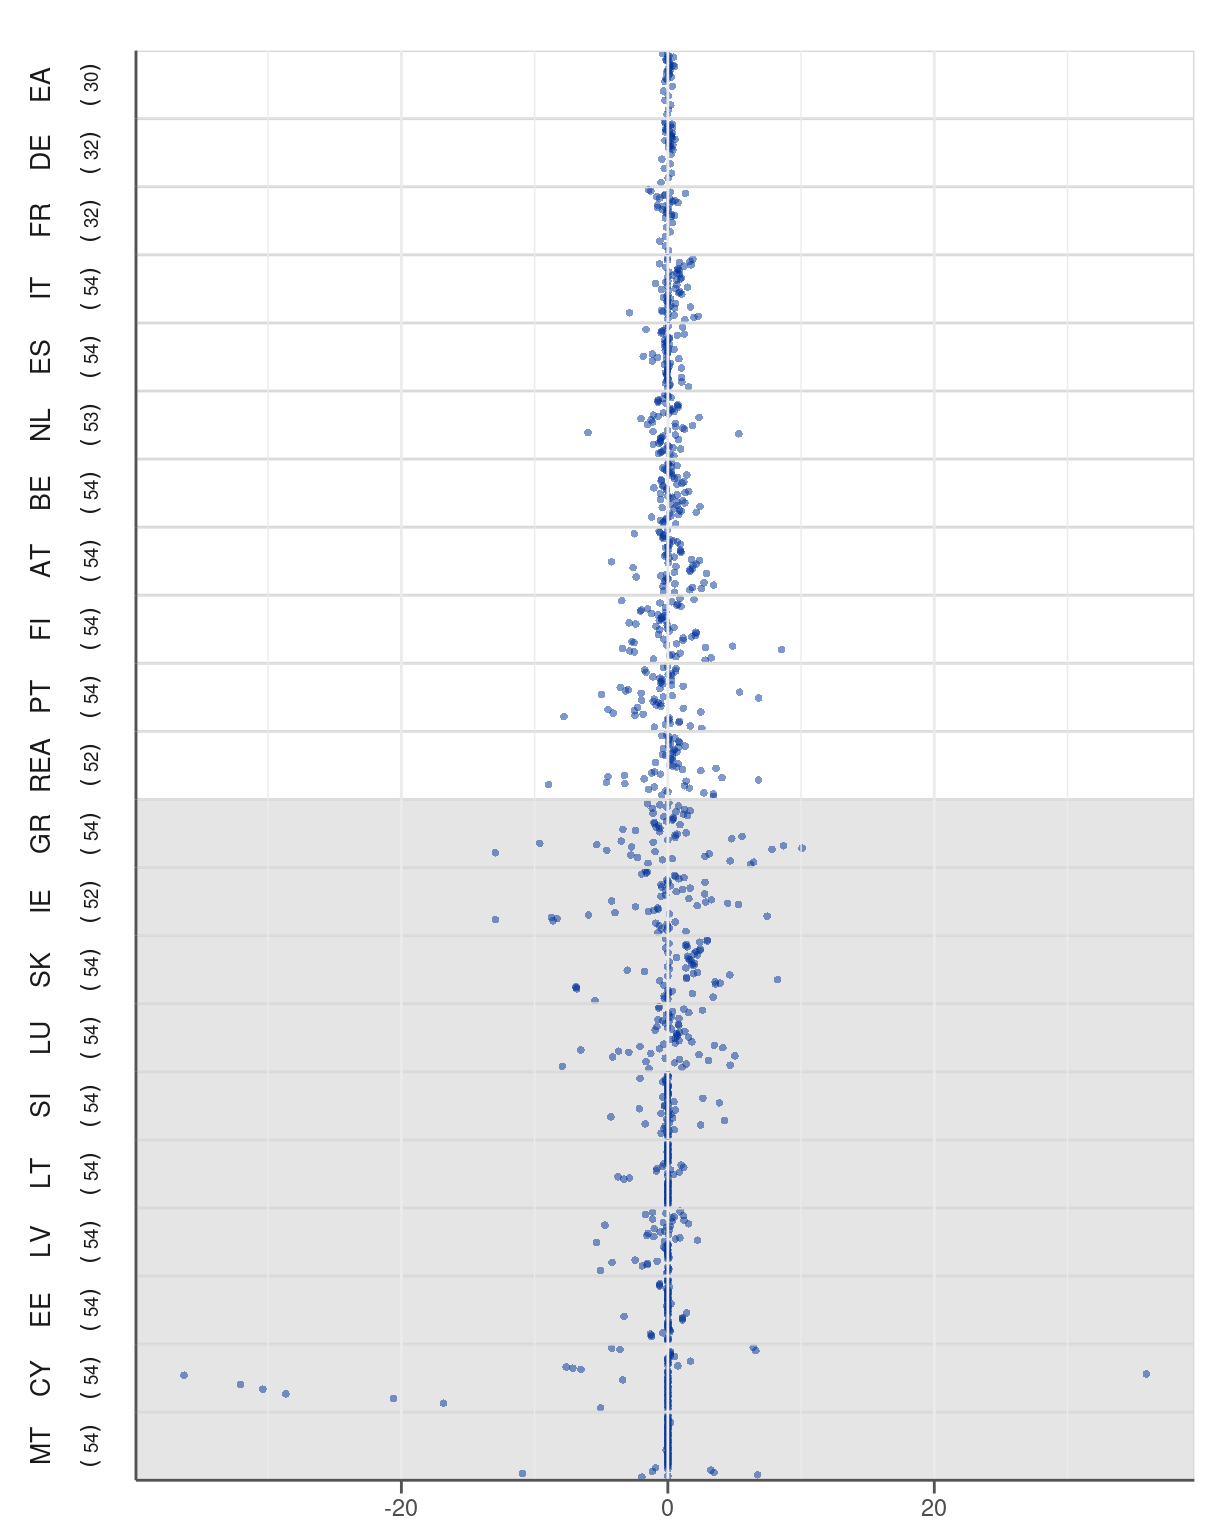
\includegraphics{./A-Graphs-revisions_files/figure-pdf/fig-SCT-1.pdf}

}

\caption{\label{fig-SCT}Final revisions to social contributions}

\end{figure}

\pagebreak

\begin{figure}[H]

{\centering 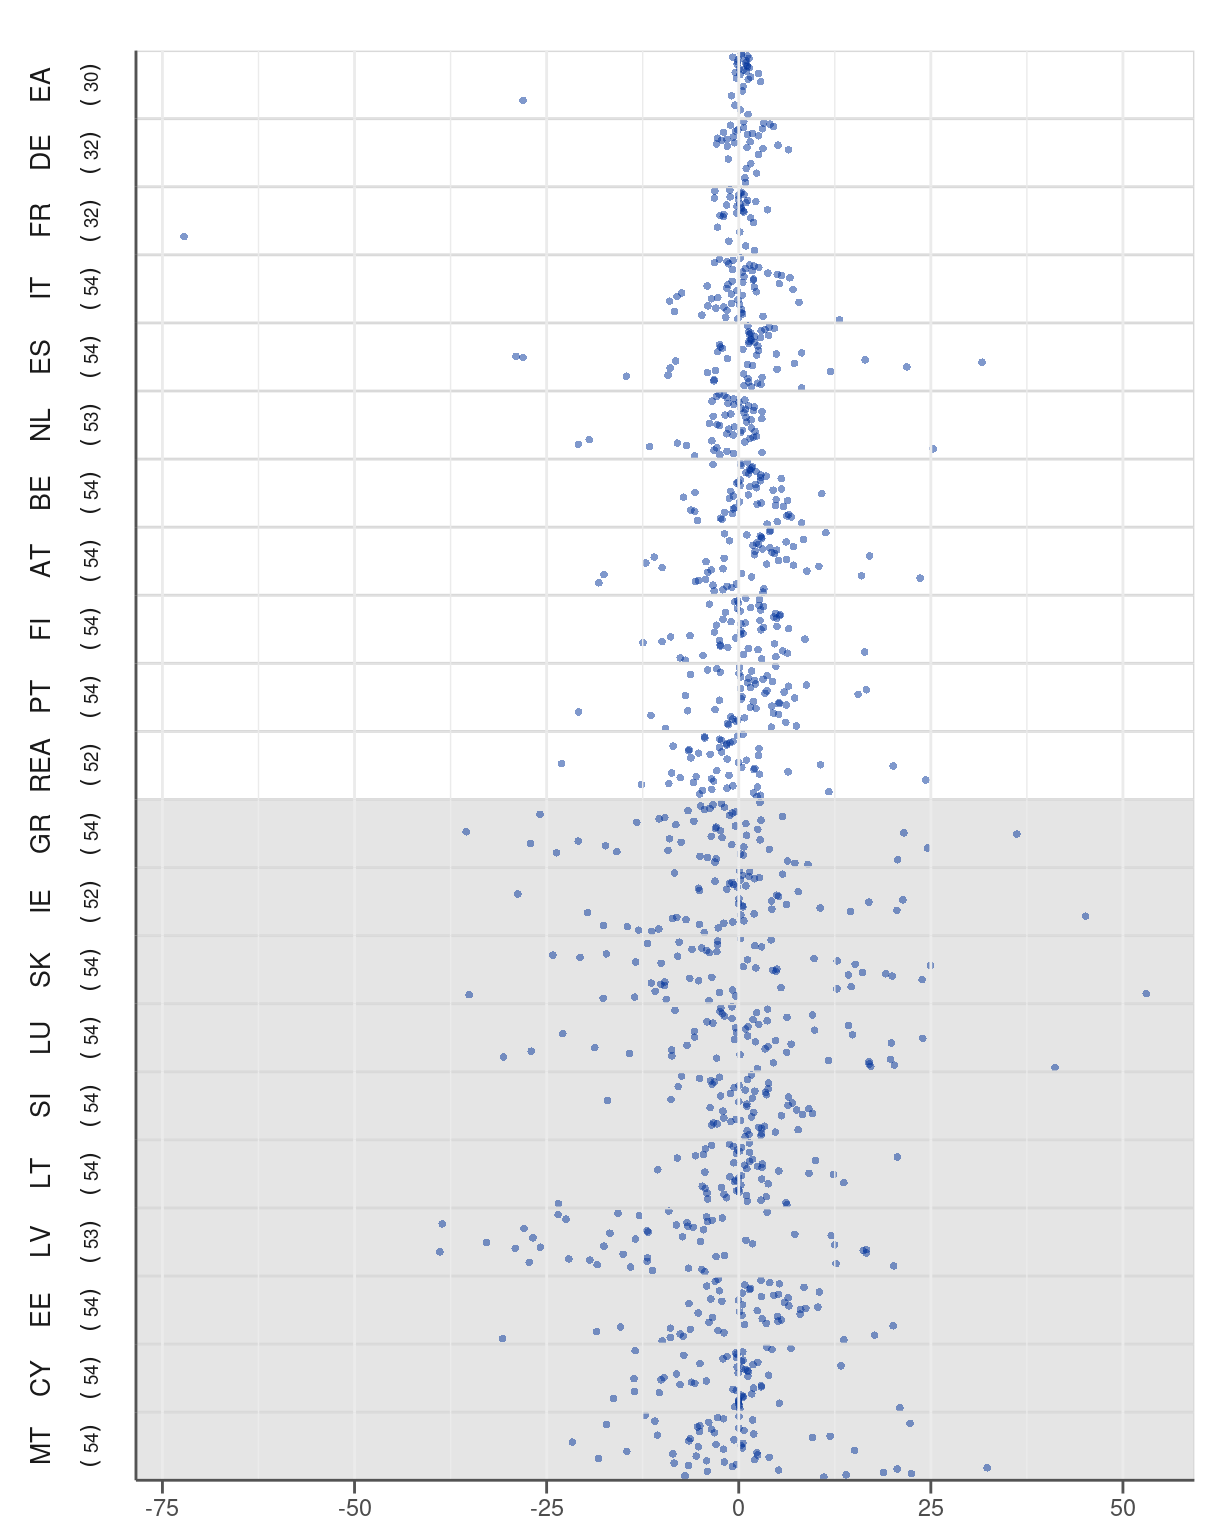
\includegraphics{./A-Graphs-revisions_files/figure-pdf/fig-OCR-1.pdf}

}

\caption{\label{fig-OCR}Final revisions to other current revenue}

\end{figure}

\pagebreak

\begin{figure}[H]

{\centering 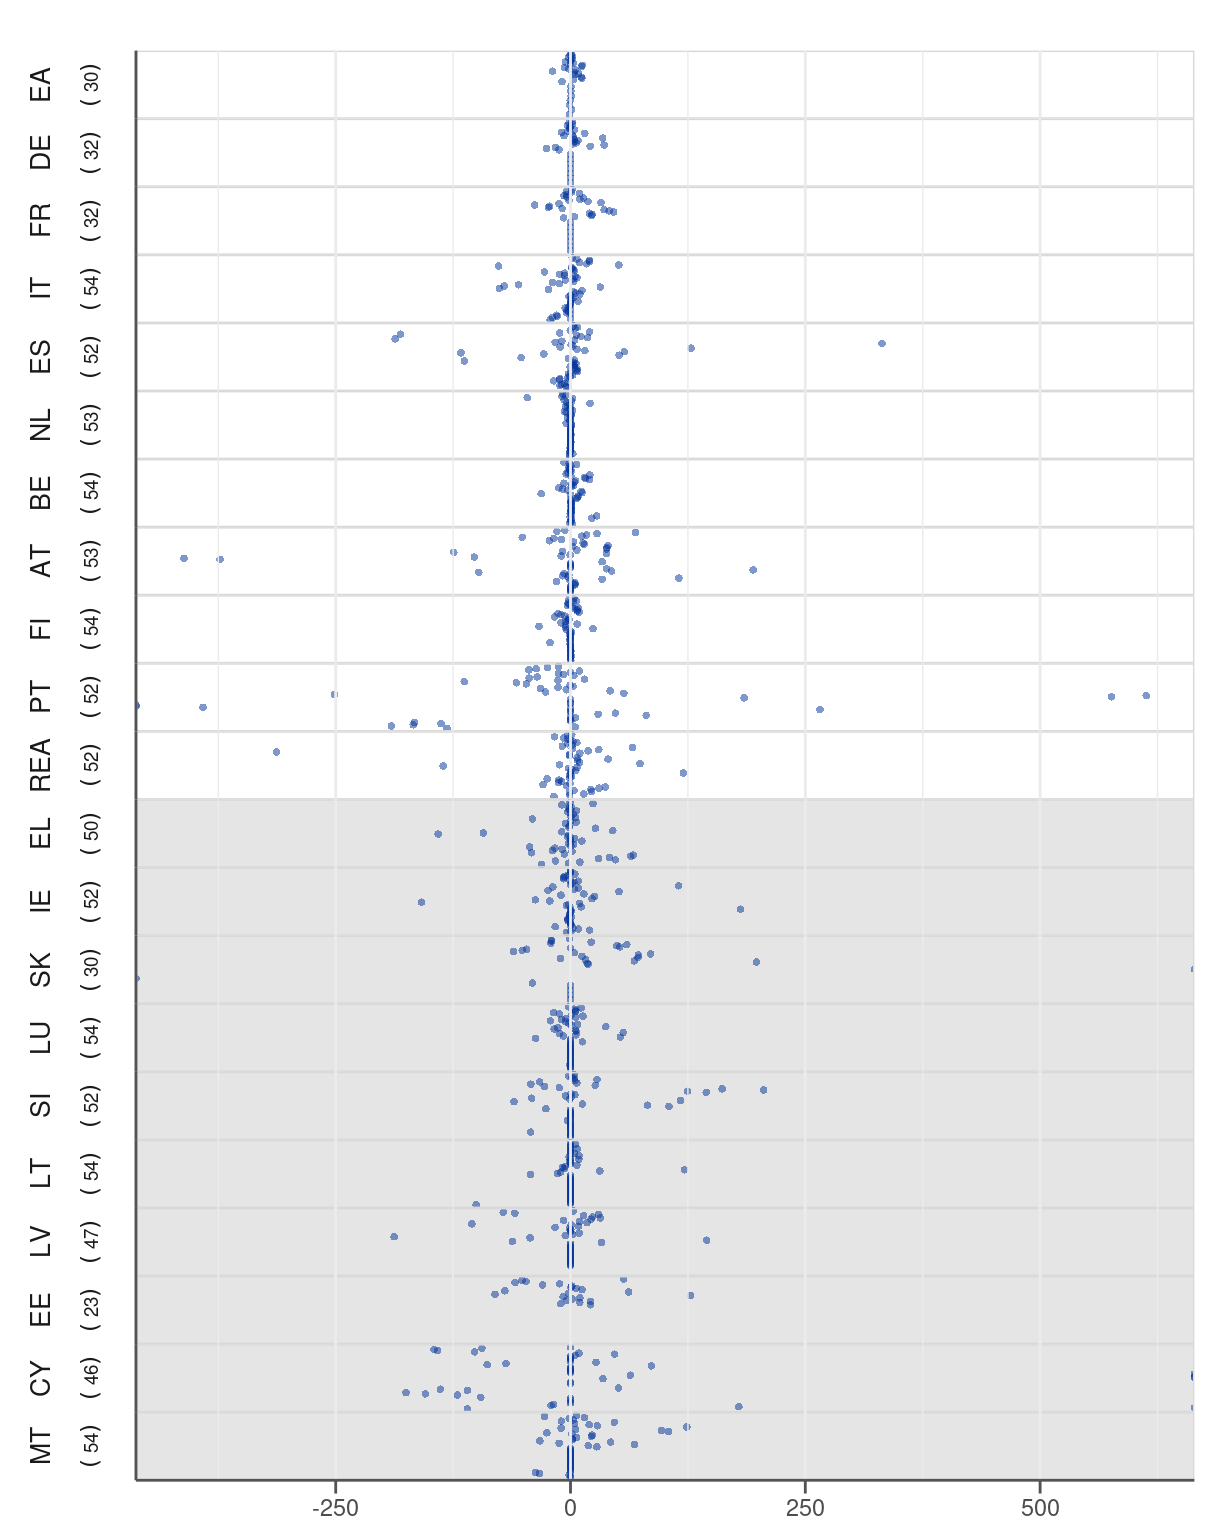
\includegraphics{./A-Graphs-revisions_files/figure-pdf/fig-KTR-1.pdf}

}

\caption{\label{fig-KTR}Final revisions to capital revenue}

\end{figure}

\hypertarget{fiscal-spending-variables}{%
\section{Fiscal spending variables}\label{fiscal-spending-variables}}

\begin{figure}[H]

{\centering 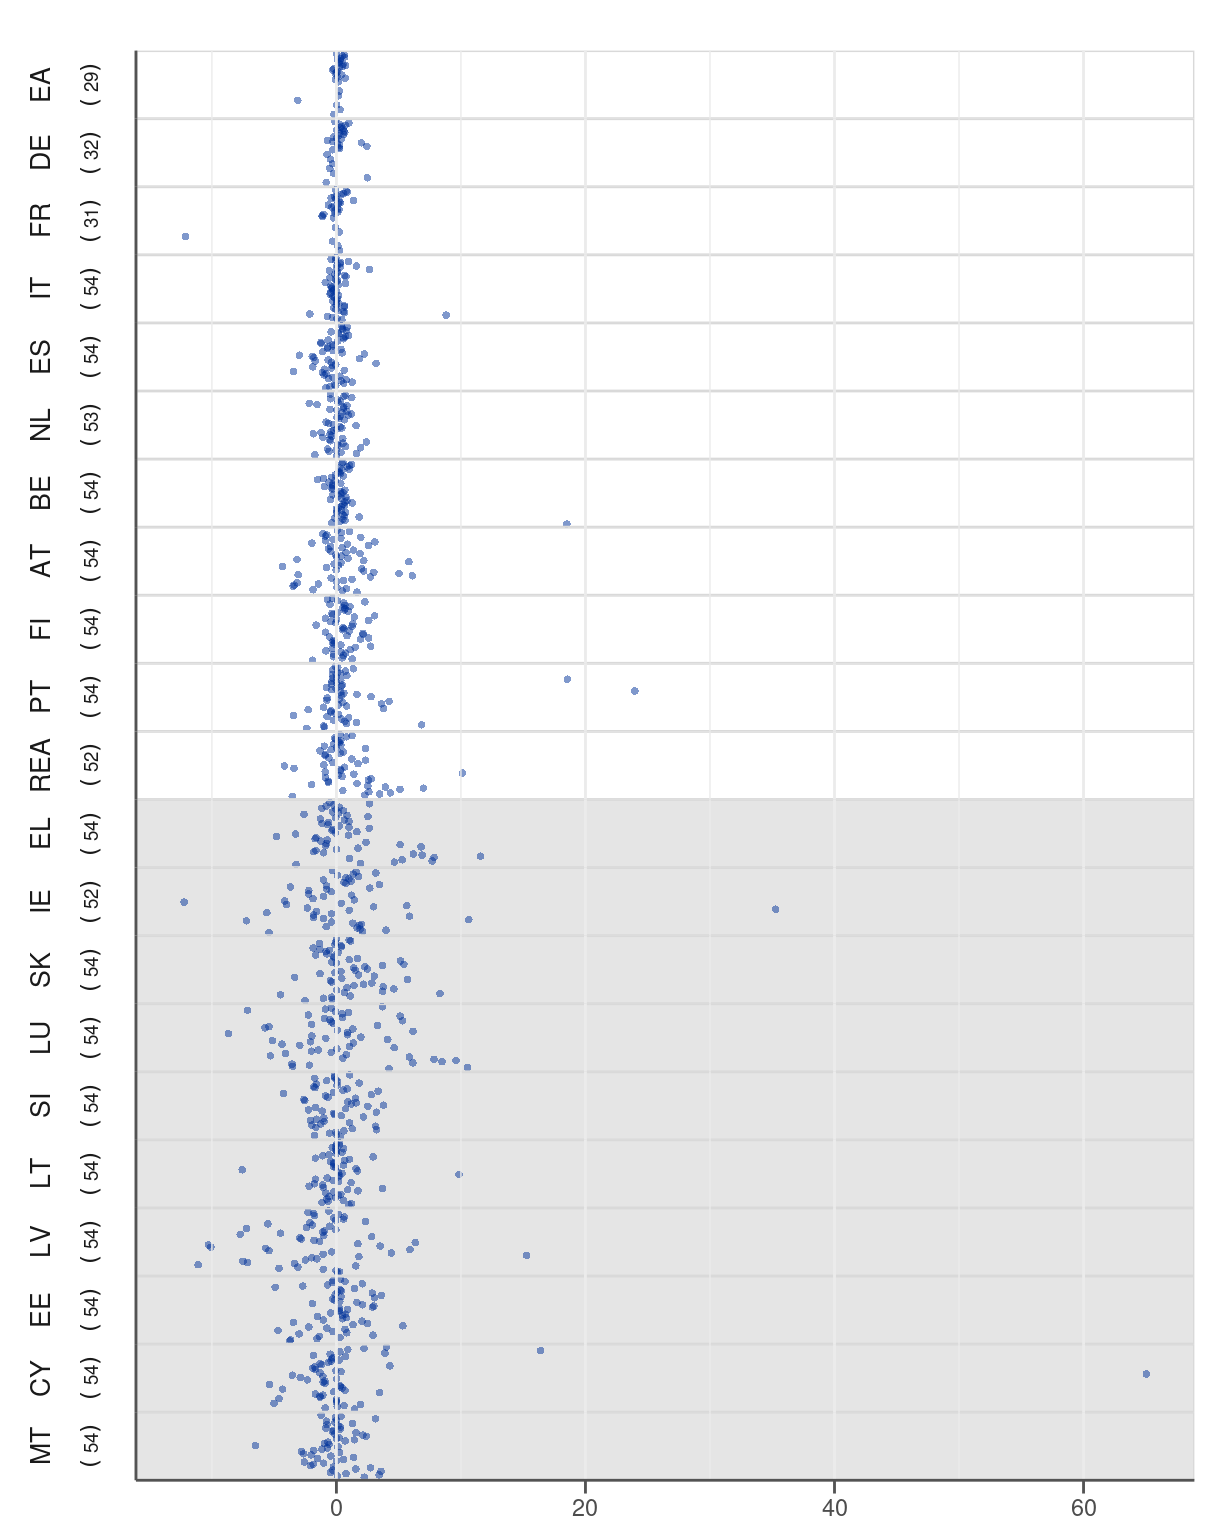
\includegraphics{./A-Graphs-revisions_files/figure-pdf/fig-TOE-1.pdf}

}

\caption{\label{fig-TOE}Final revisions to total expenditure}

\end{figure}

\pagebreak

\begin{figure}[H]

{\centering 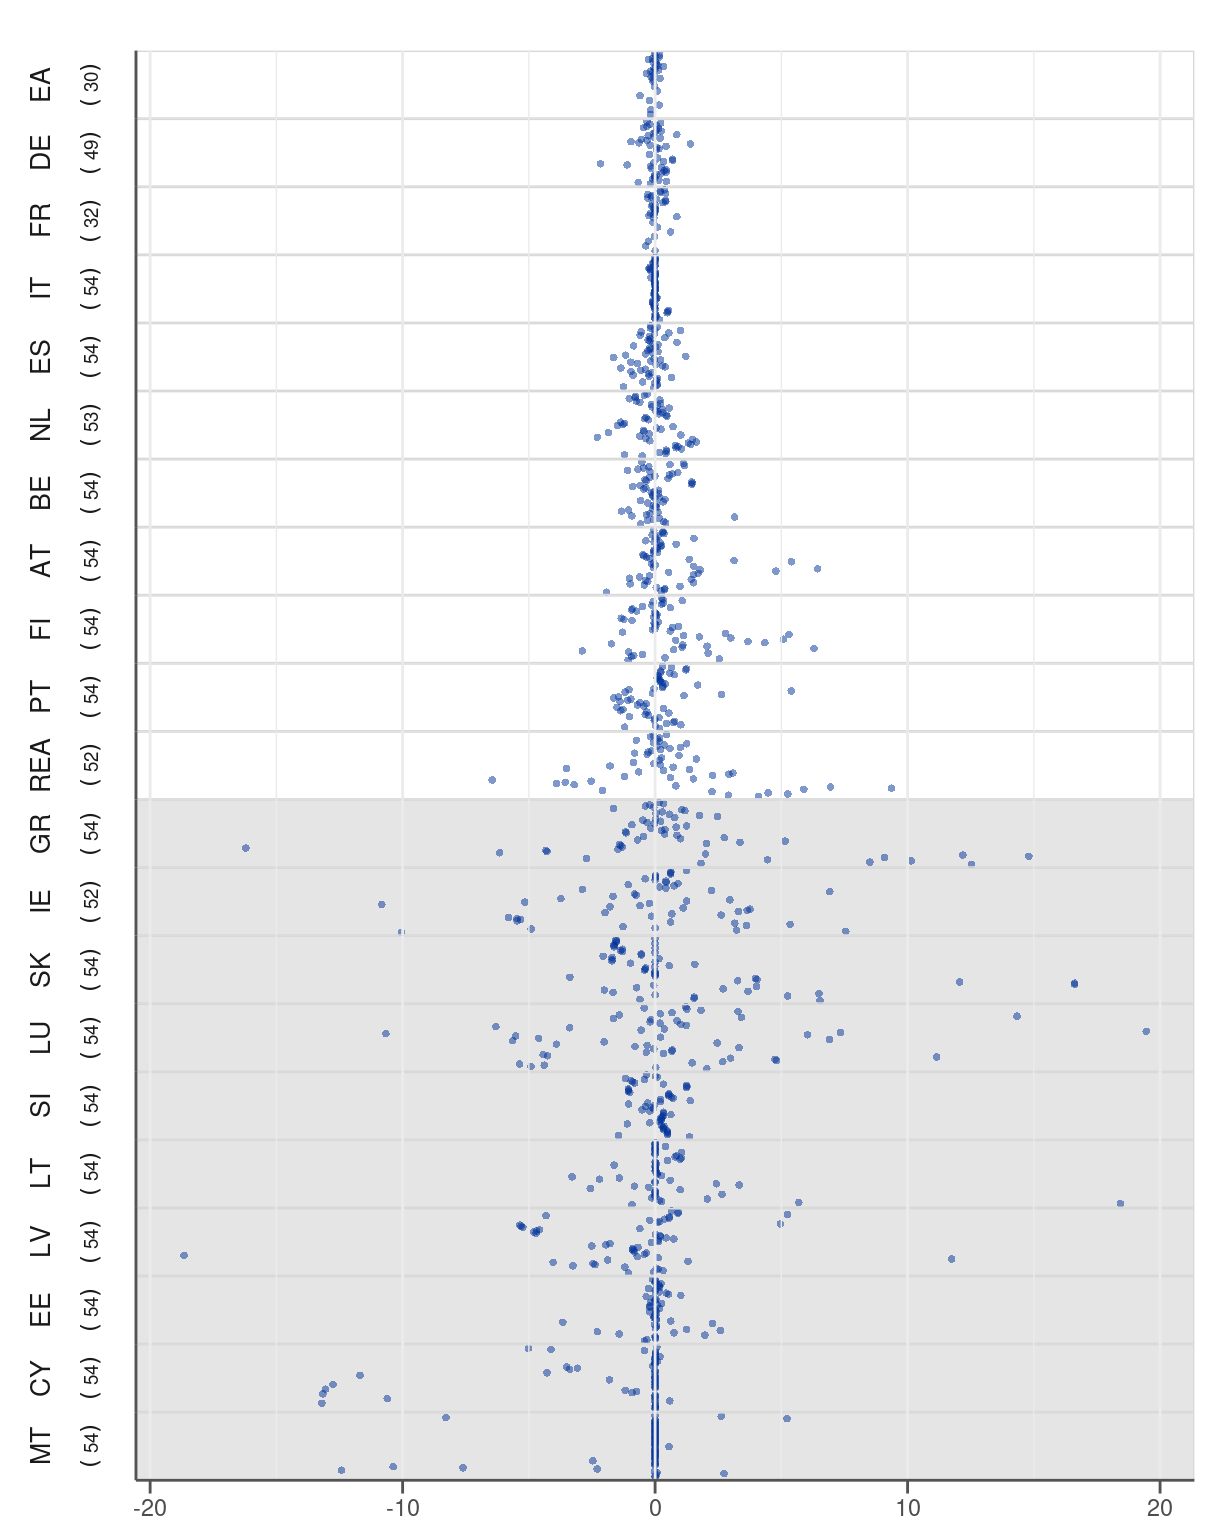
\includegraphics{./A-Graphs-revisions_files/figure-pdf/fig-THN-1.pdf}

}

\caption{\label{fig-THN}Final revisions to social transfers}

\end{figure}

\pagebreak

\begin{figure}[H]

{\centering 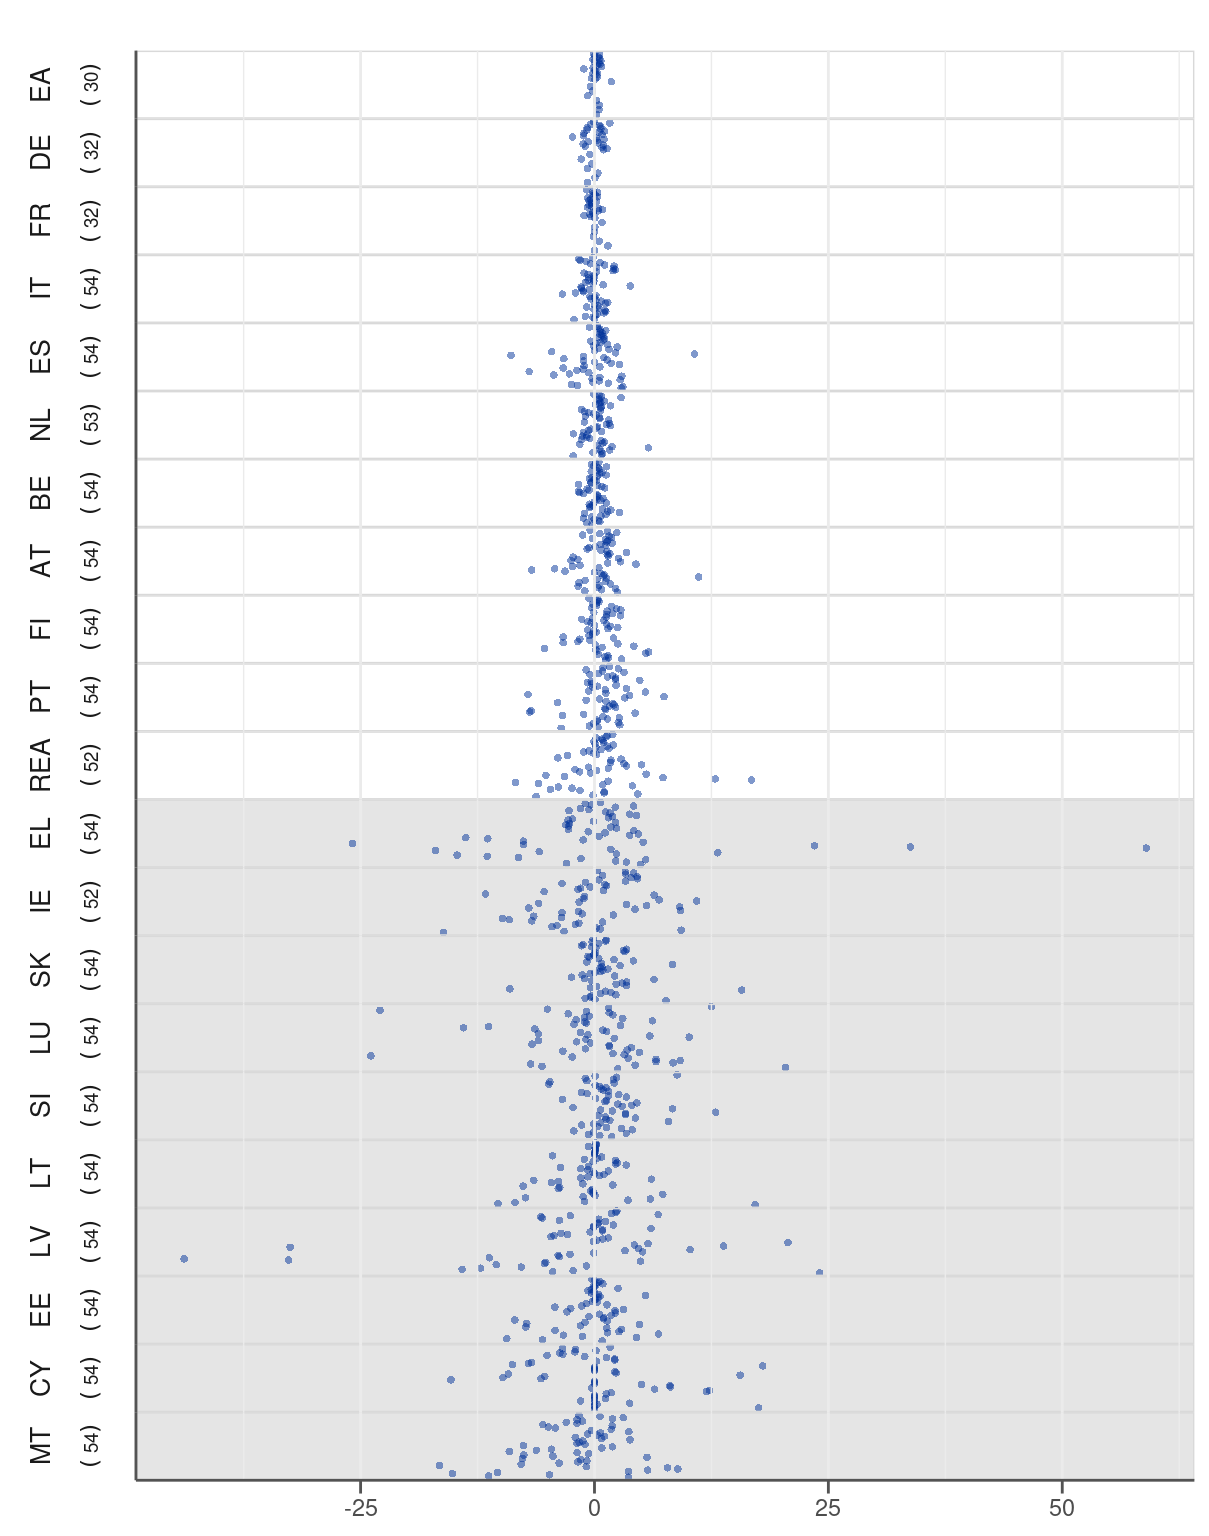
\includegraphics{./A-Graphs-revisions_files/figure-pdf/fig-PUR-1.pdf}

}

\caption{\label{fig-PUR}Final revisions to purchases}

\end{figure}

\pagebreak

\begin{figure}[H]

{\centering 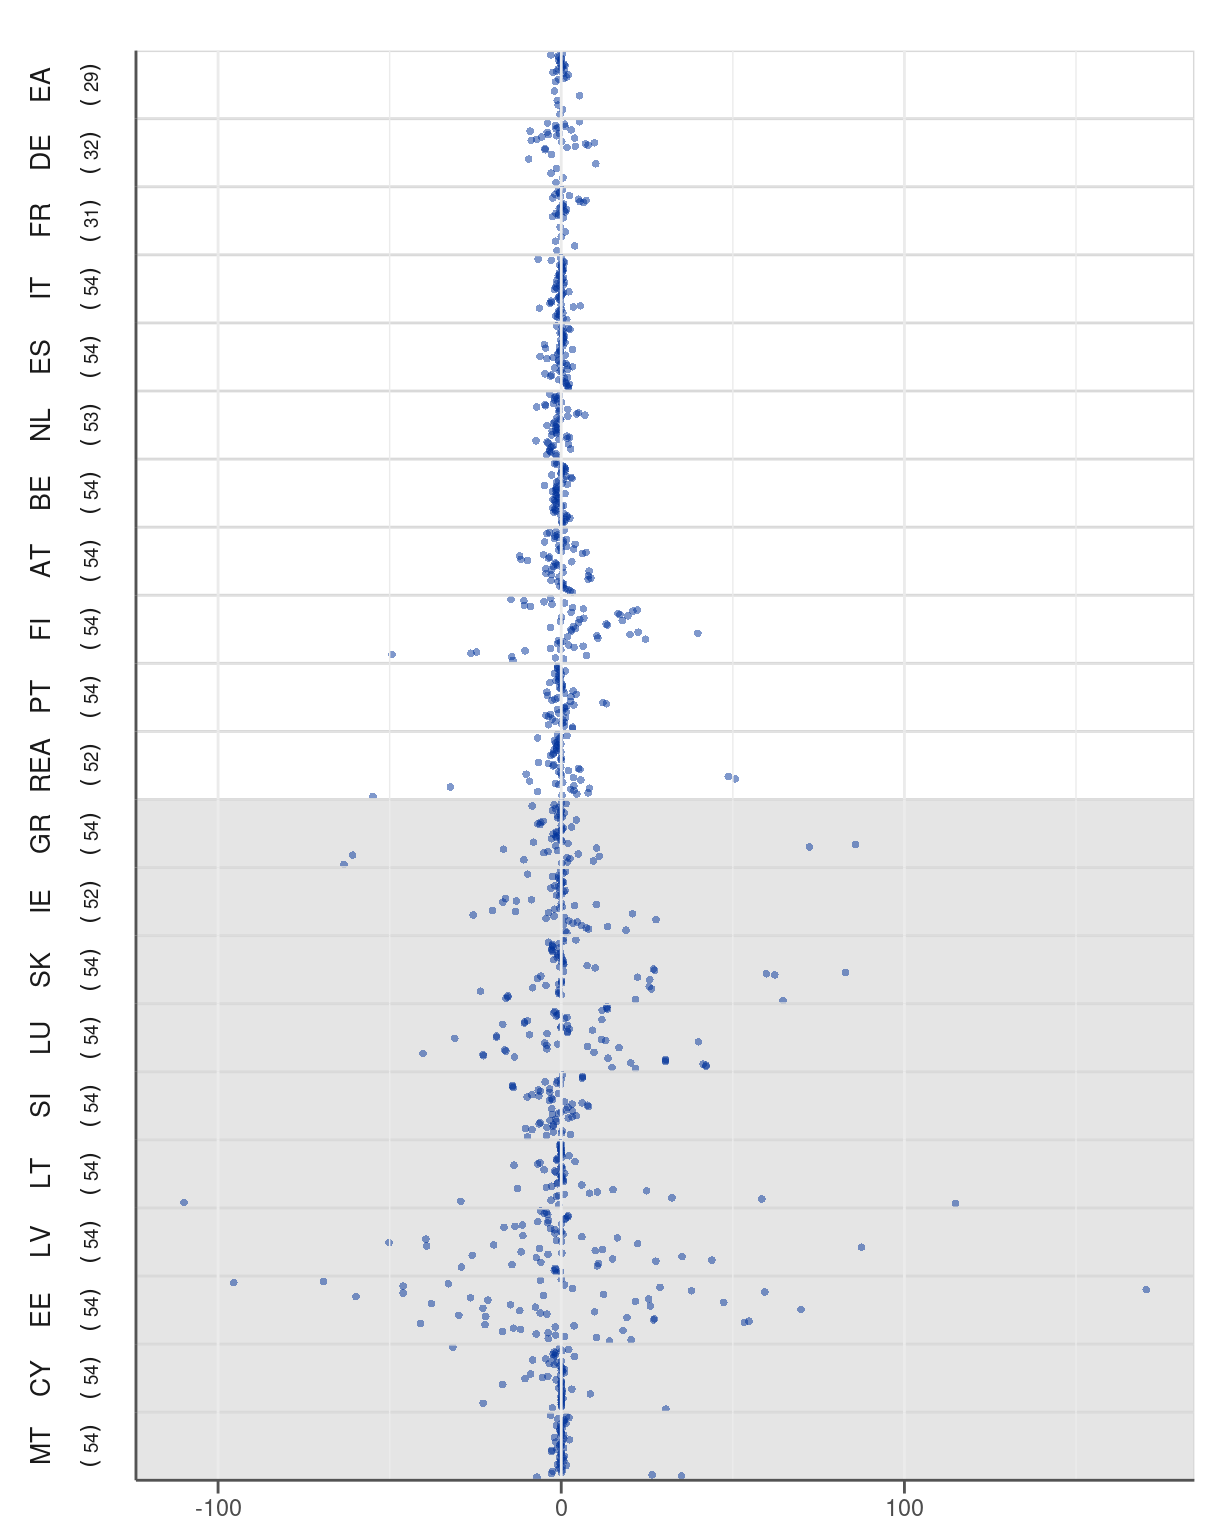
\includegraphics{./A-Graphs-revisions_files/figure-pdf/fig-INP-1.pdf}

}

\caption{\label{fig-INP}Final revisions to interest payments}

\end{figure}

\pagebreak

\begin{figure}[H]

{\centering 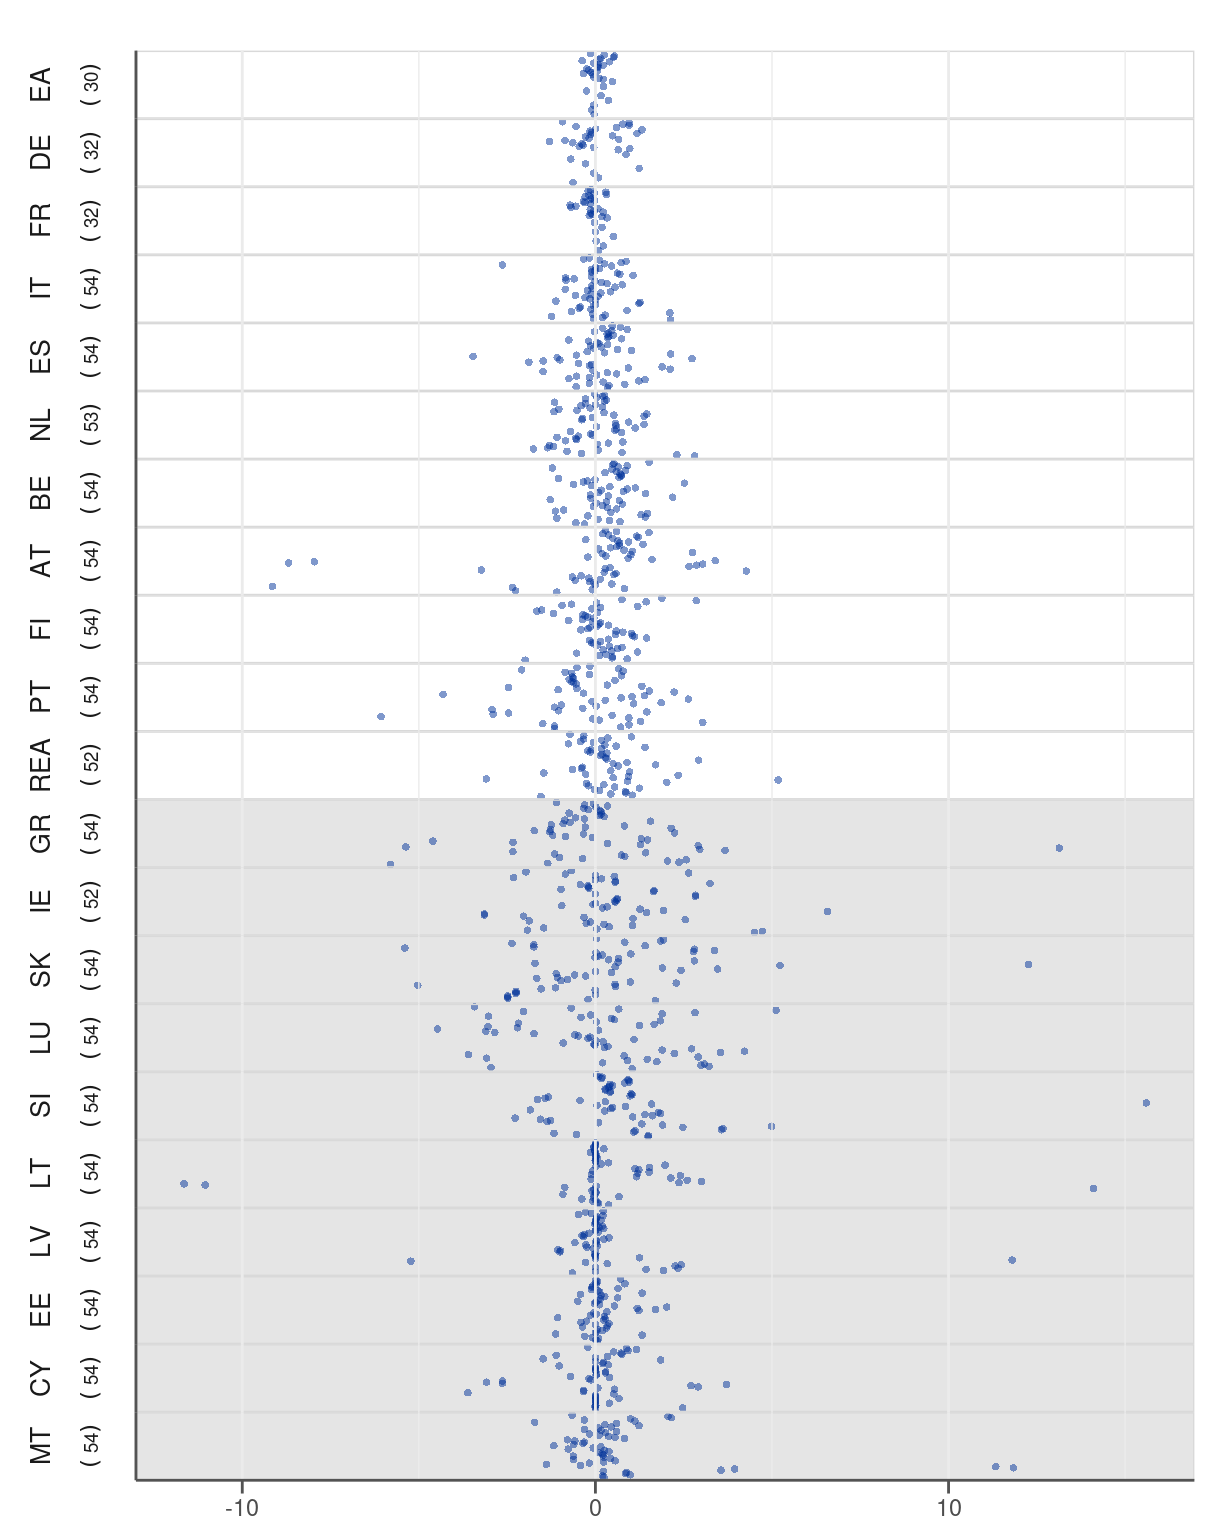
\includegraphics{./A-Graphs-revisions_files/figure-pdf/fig-COE-1.pdf}

}

\caption{\label{fig-COE}Final revisions to gov. compensation}

\end{figure}

\pagebreak

\begin{figure}[H]

{\centering 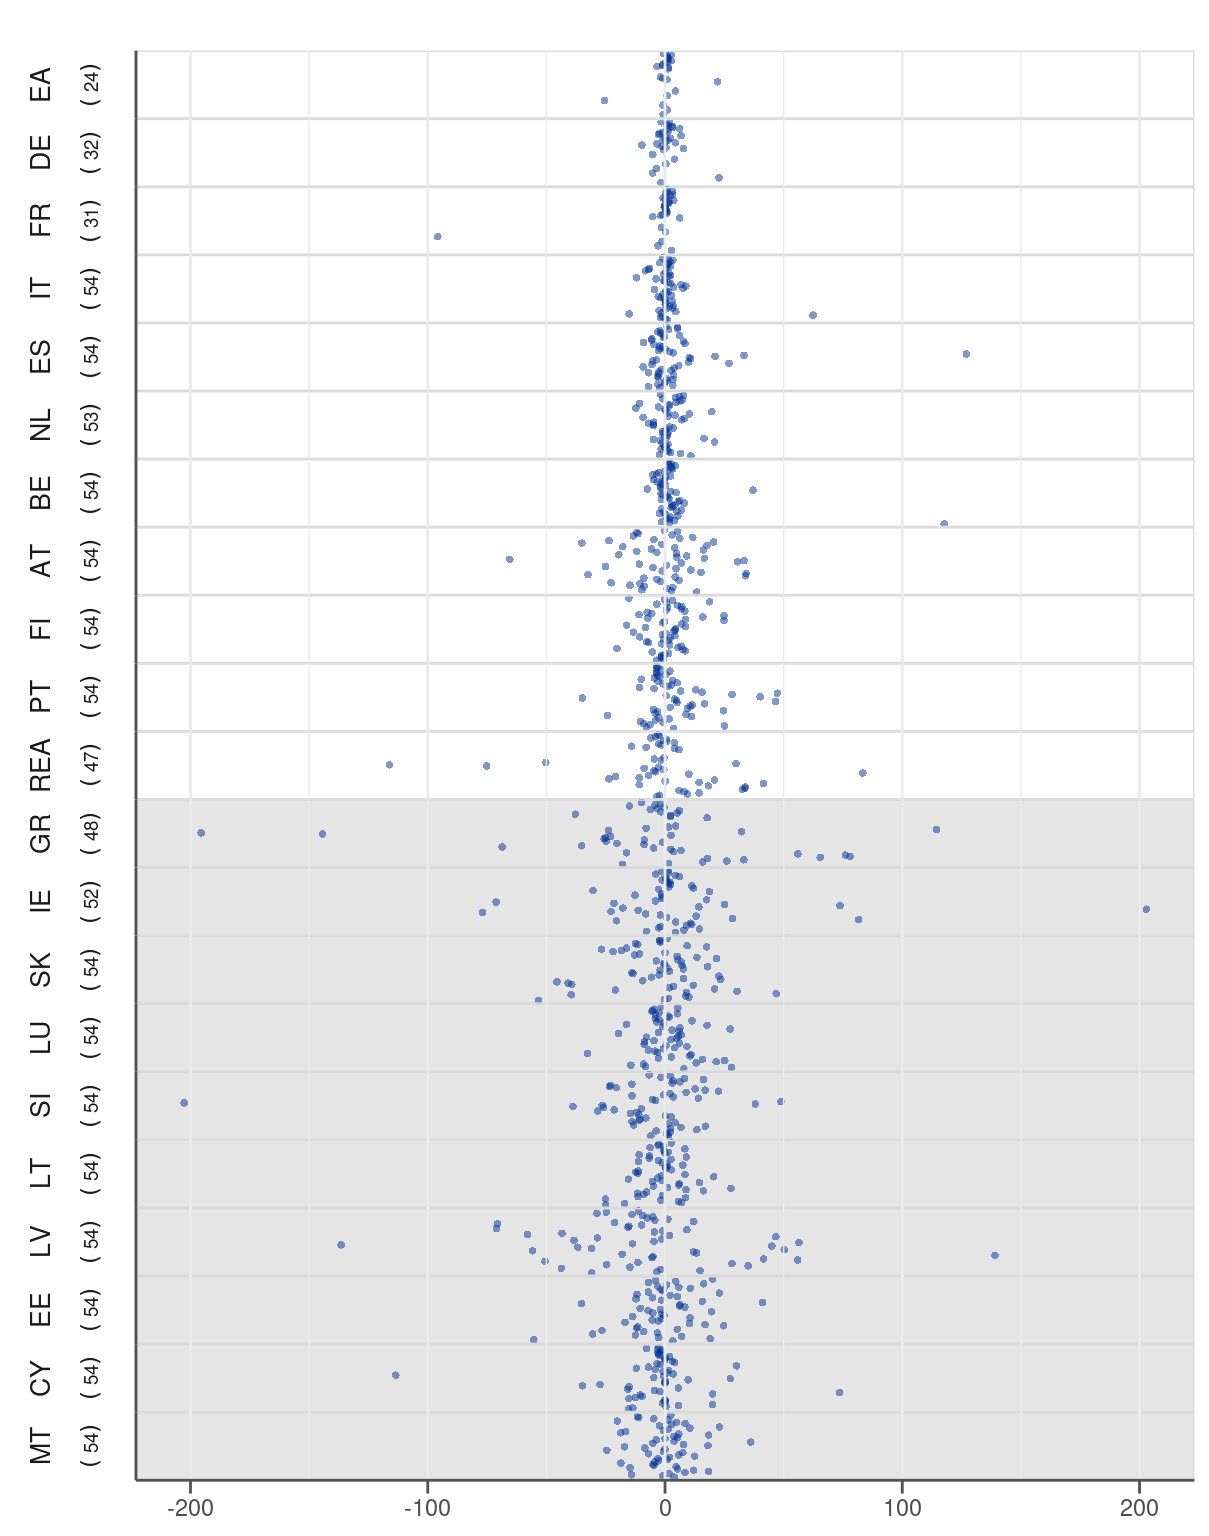
\includegraphics{./A-Graphs-revisions_files/figure-pdf/fig-OCE-1.pdf}

}

\caption{\label{fig-OCE}Final revisions to other current expenditure}

\end{figure}

\pagebreak

\begin{figure}[H]

{\centering 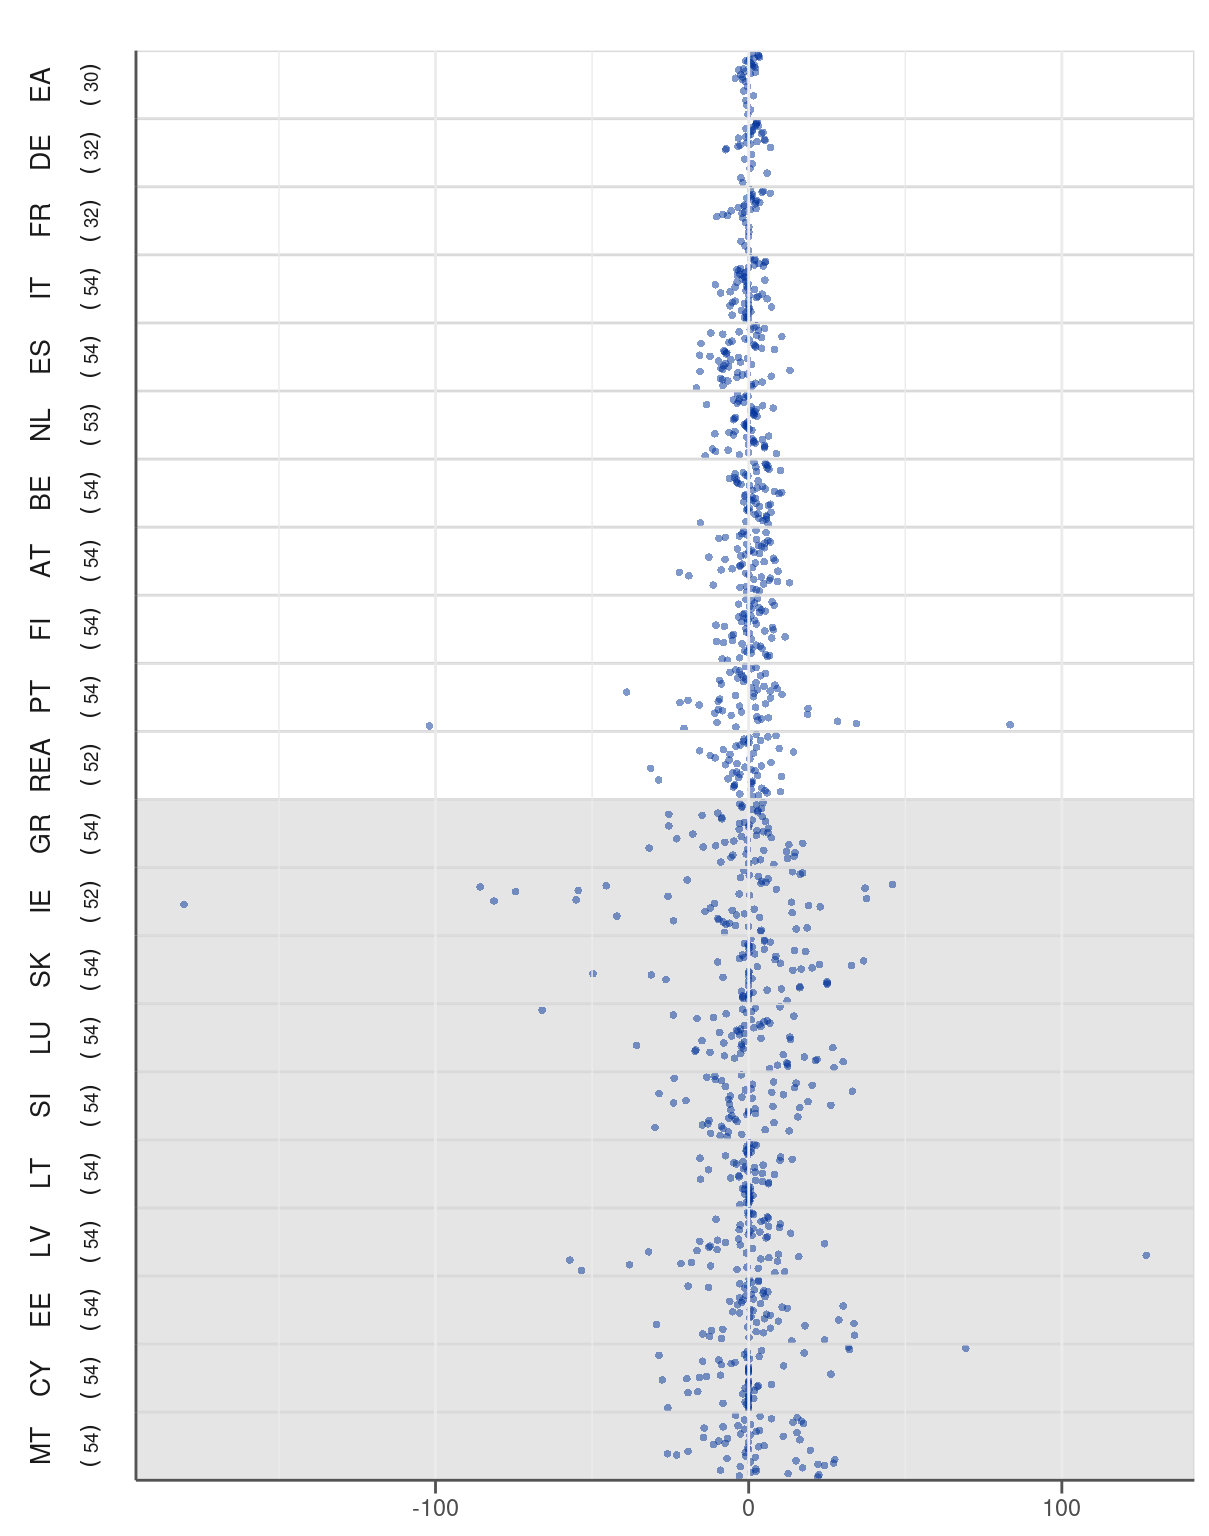
\includegraphics{./A-Graphs-revisions_files/figure-pdf/fig-GIN-1.pdf}

}

\caption{\label{fig-GIN}Final revisions to gov. investment}

\end{figure}

\pagebreak

\begin{figure}[H]

{\centering 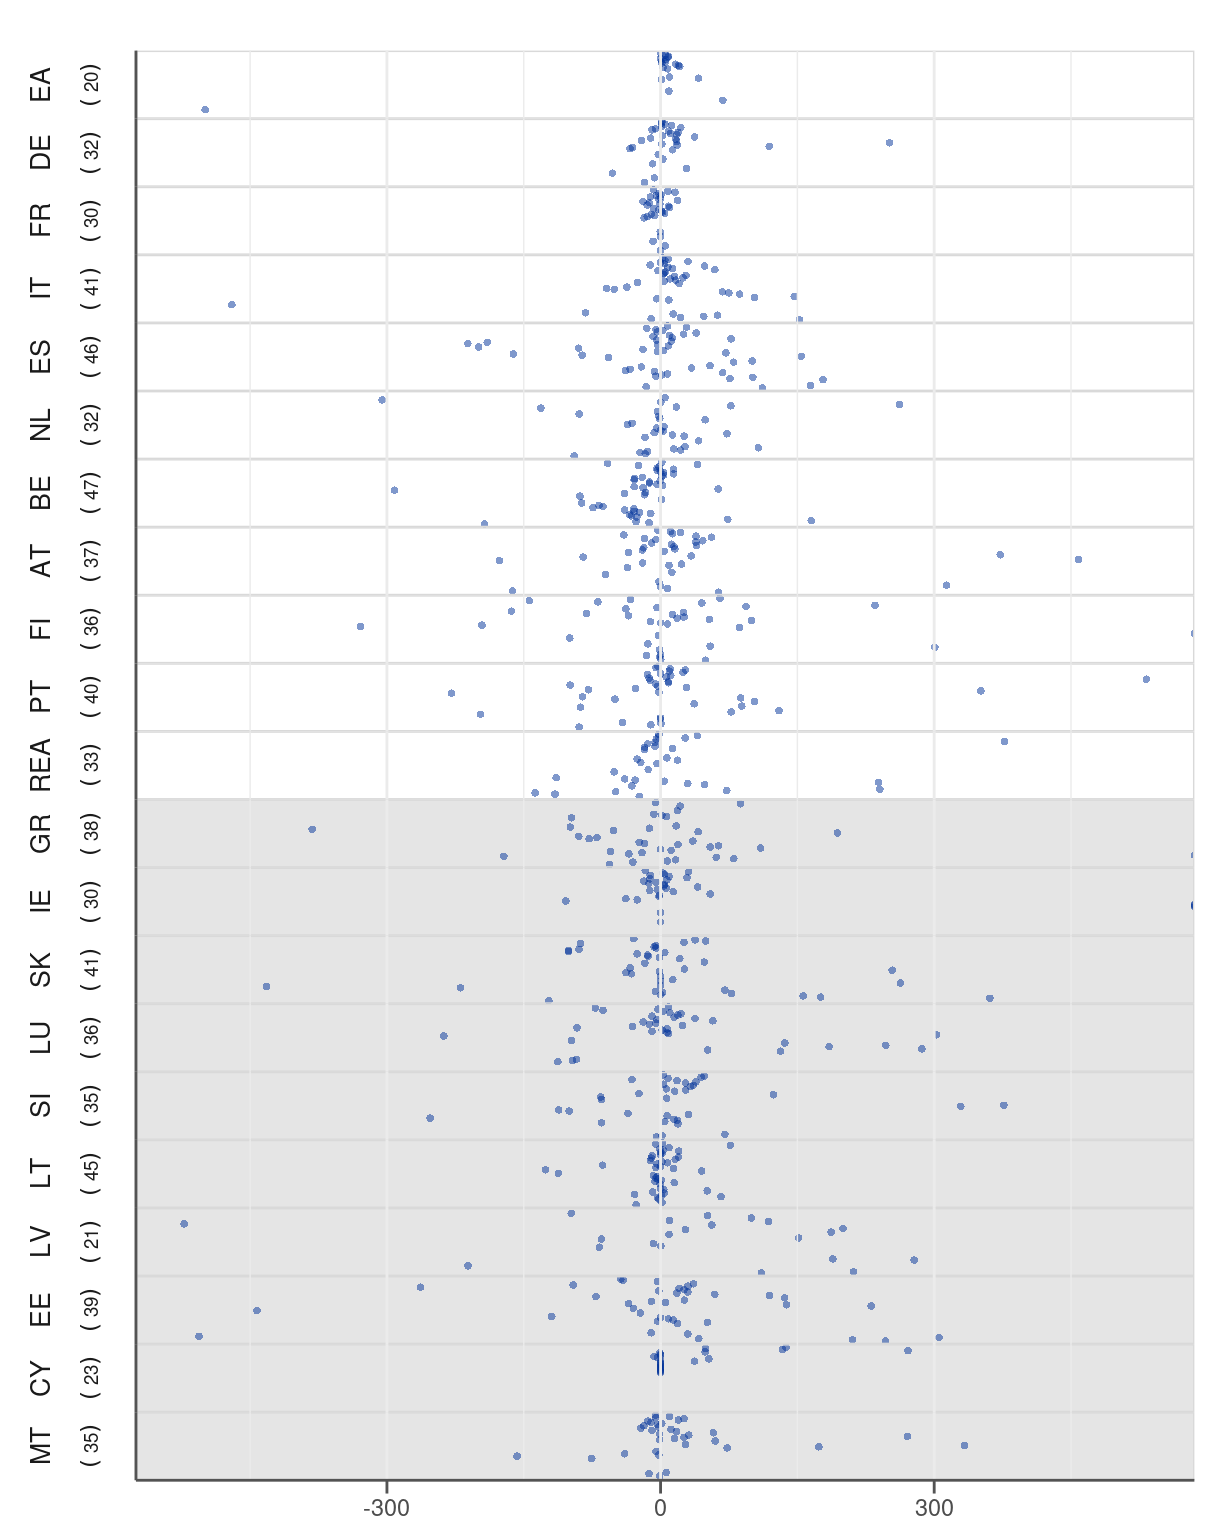
\includegraphics{./A-Graphs-revisions_files/figure-pdf/fig-OKE-1.pdf}

}

\caption{\label{fig-OKE}Final revisions to other capital expenditure}

\end{figure}

\hypertarget{macro-variables}{%
\section{Macro variables}\label{macro-variables}}

\begin{figure}[H]

{\centering 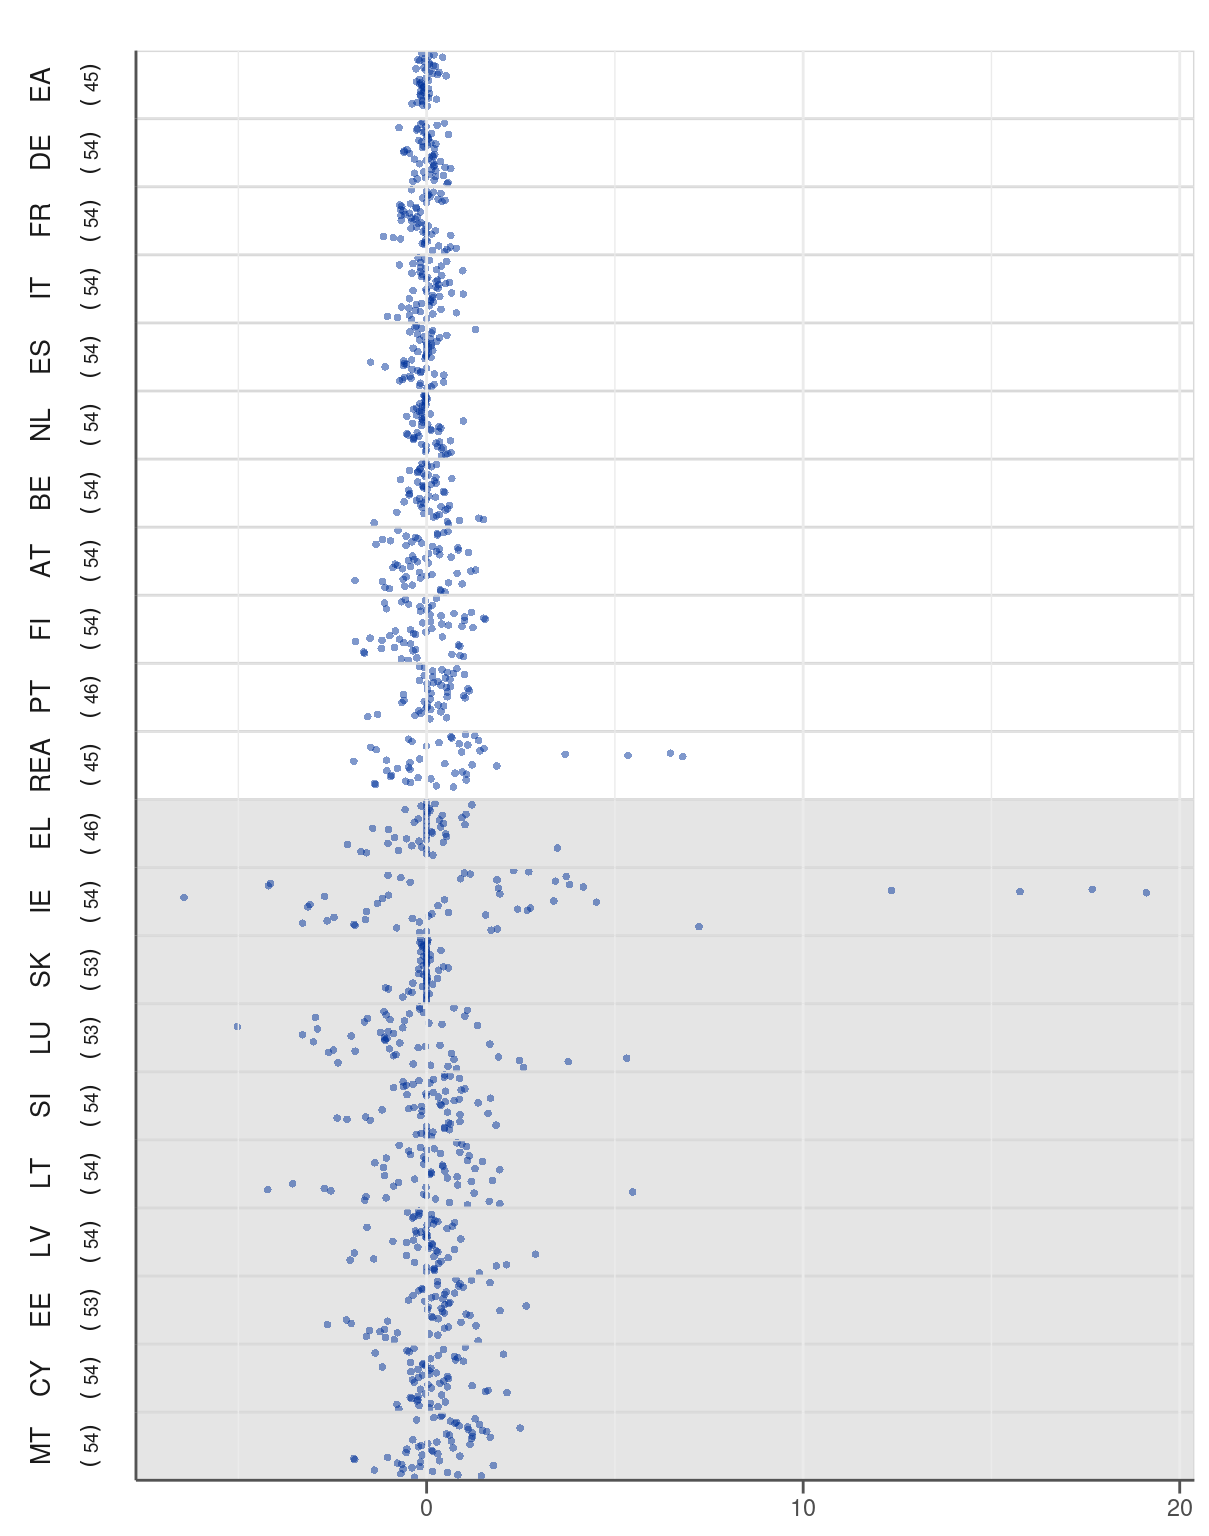
\includegraphics{./A-Graphs-revisions_files/figure-pdf/fig-YEN-1.pdf}

}

\caption{\label{fig-YEN}Final revisions to GDP}

\end{figure}

\pagebreak

\begin{figure}[H]

{\centering 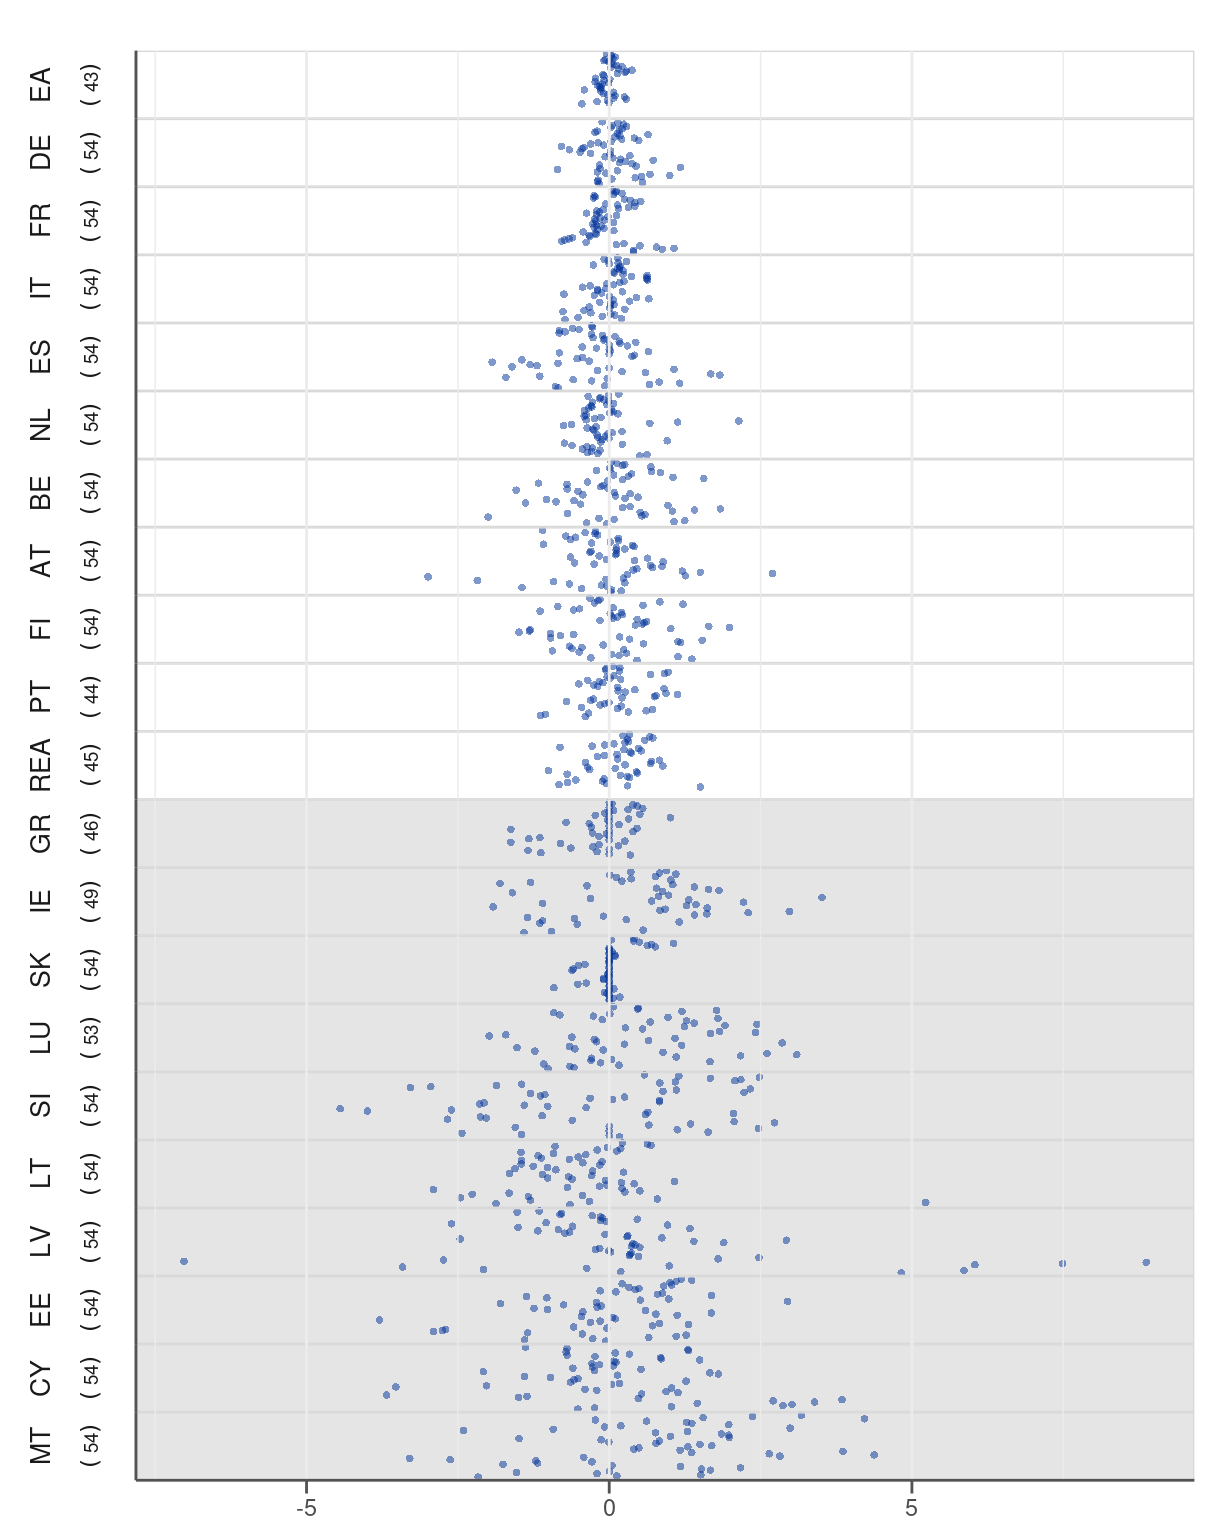
\includegraphics{./A-Graphs-revisions_files/figure-pdf/fig-PCN-1.pdf}

}

\caption{\label{fig-PCN}Final revisions to private consumption}

\end{figure}

\pagebreak

\begin{figure}[H]

{\centering 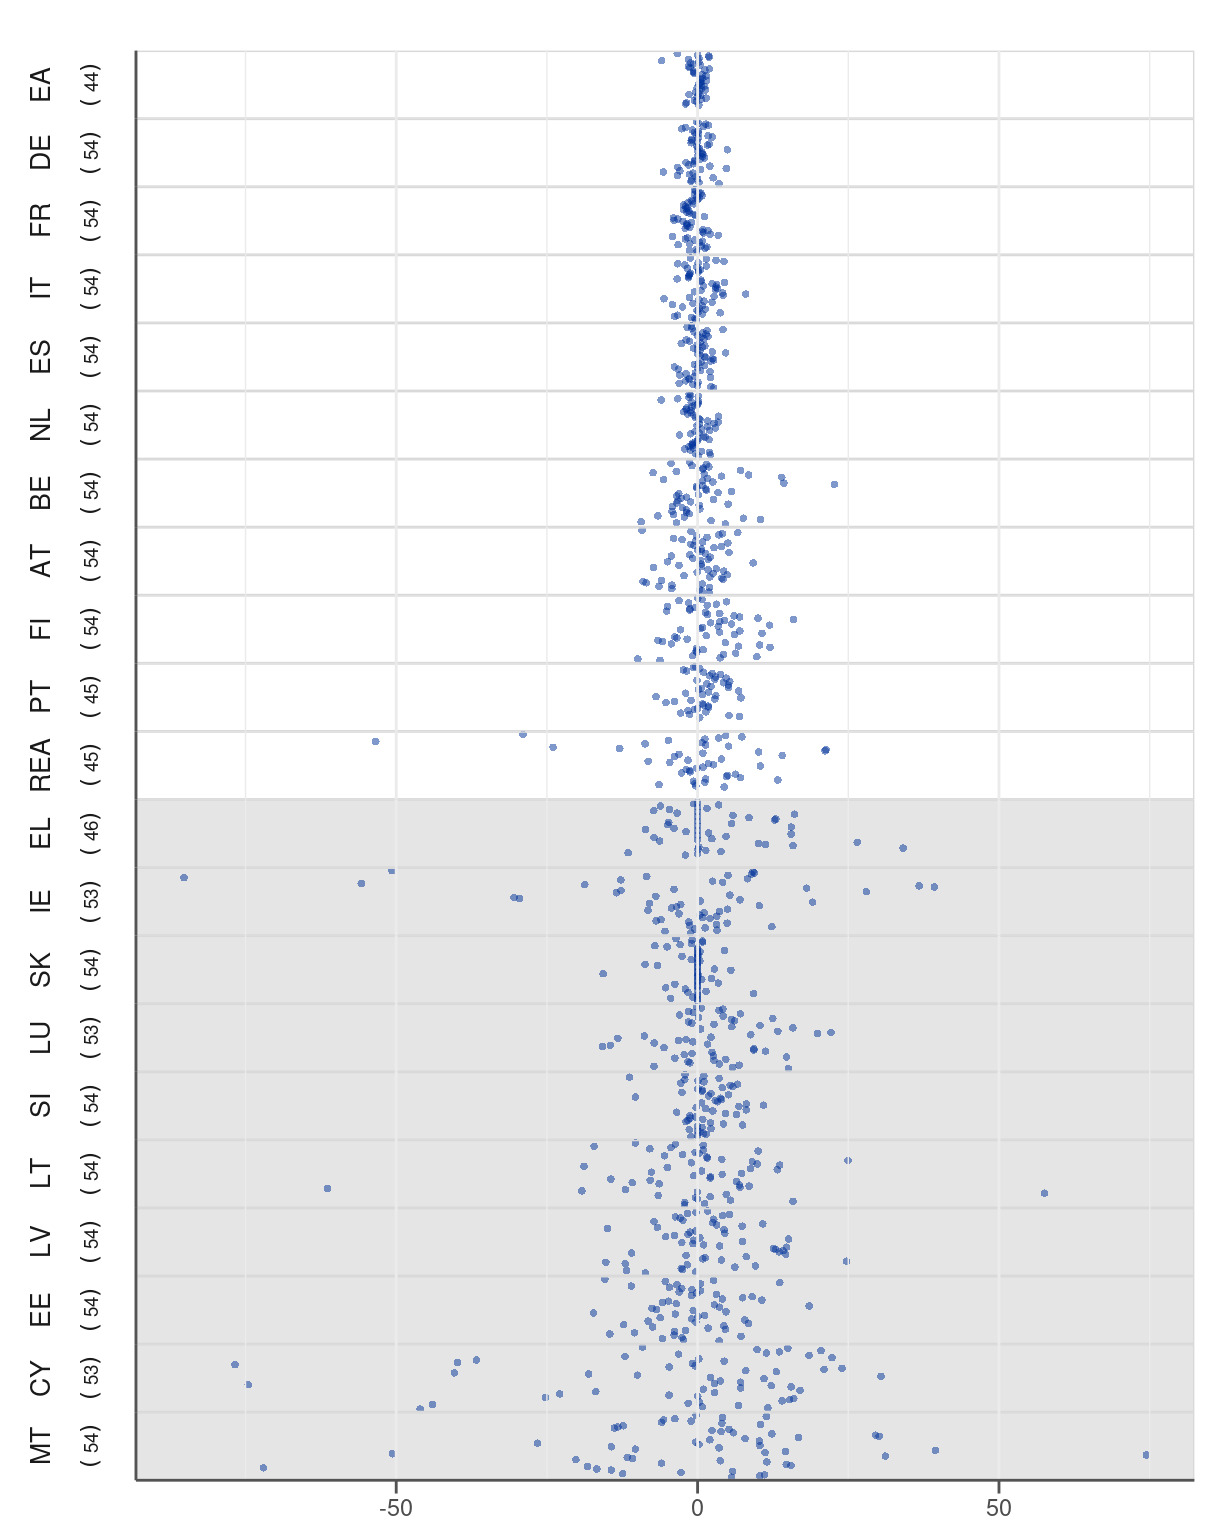
\includegraphics{./A-Graphs-revisions_files/figure-pdf/fig-ITN-1.pdf}

}

\caption{\label{fig-ITN}Final revisions to total investment}

\end{figure}

\pagebreak

\begin{figure}[H]

{\centering 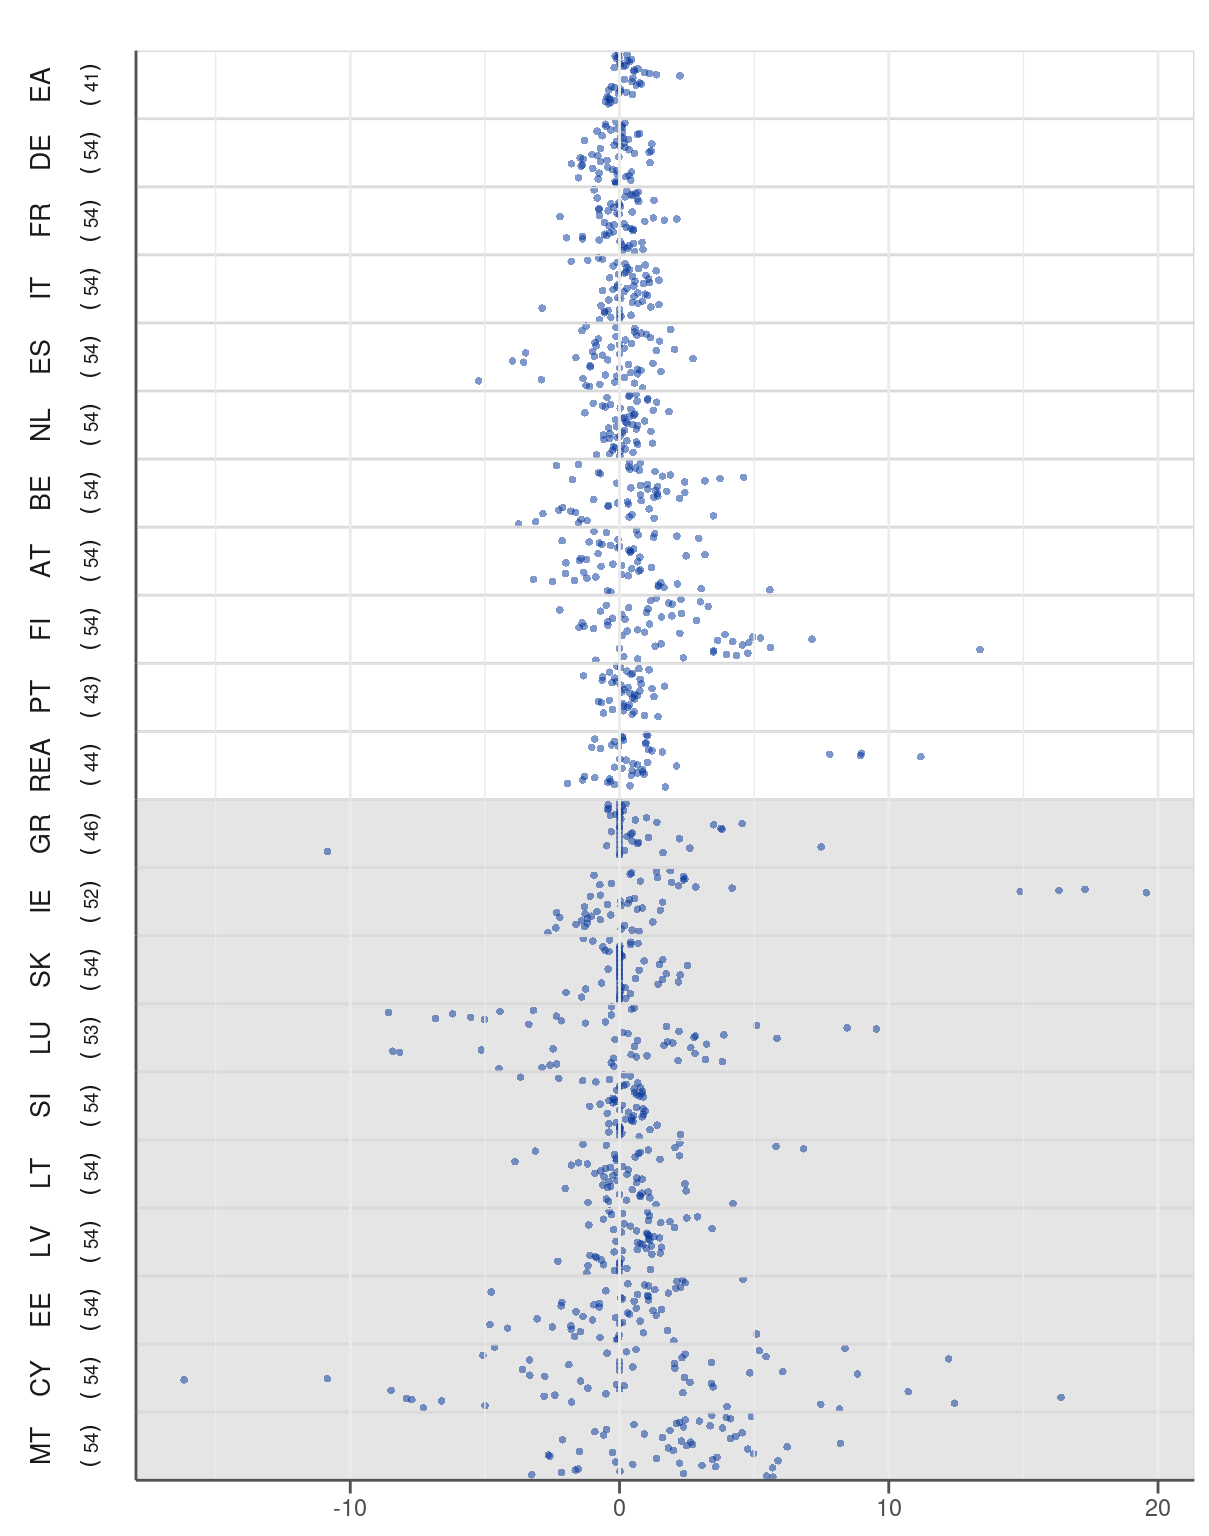
\includegraphics{./A-Graphs-revisions_files/figure-pdf/fig-EXN-1.pdf}

}

\caption{\label{fig-EXN}Final revisions to exports}

\end{figure}

\pagebreak

\begin{figure}[H]

{\centering 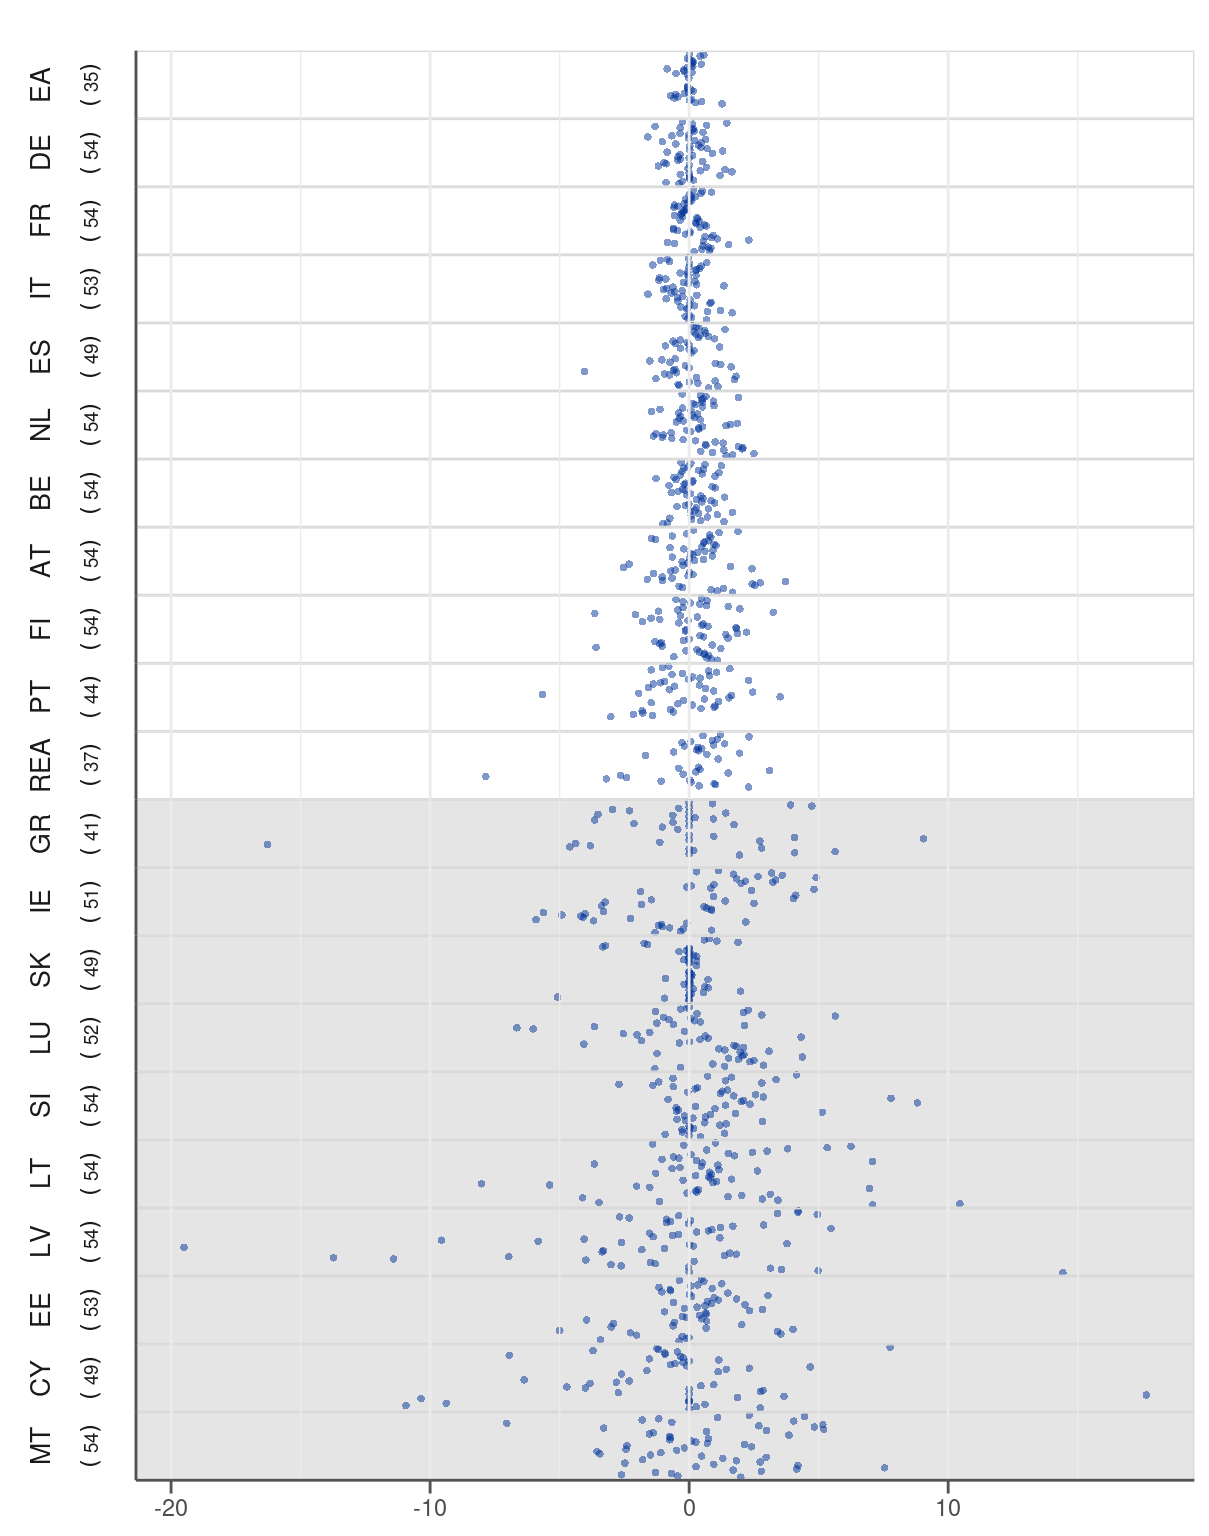
\includegraphics{./A-Graphs-revisions_files/figure-pdf/fig-GCN-1.pdf}

}

\caption{\label{fig-GCN}Final revisions to gov. consumption}

\end{figure}

\pagebreak

\begin{figure}[H]

{\centering 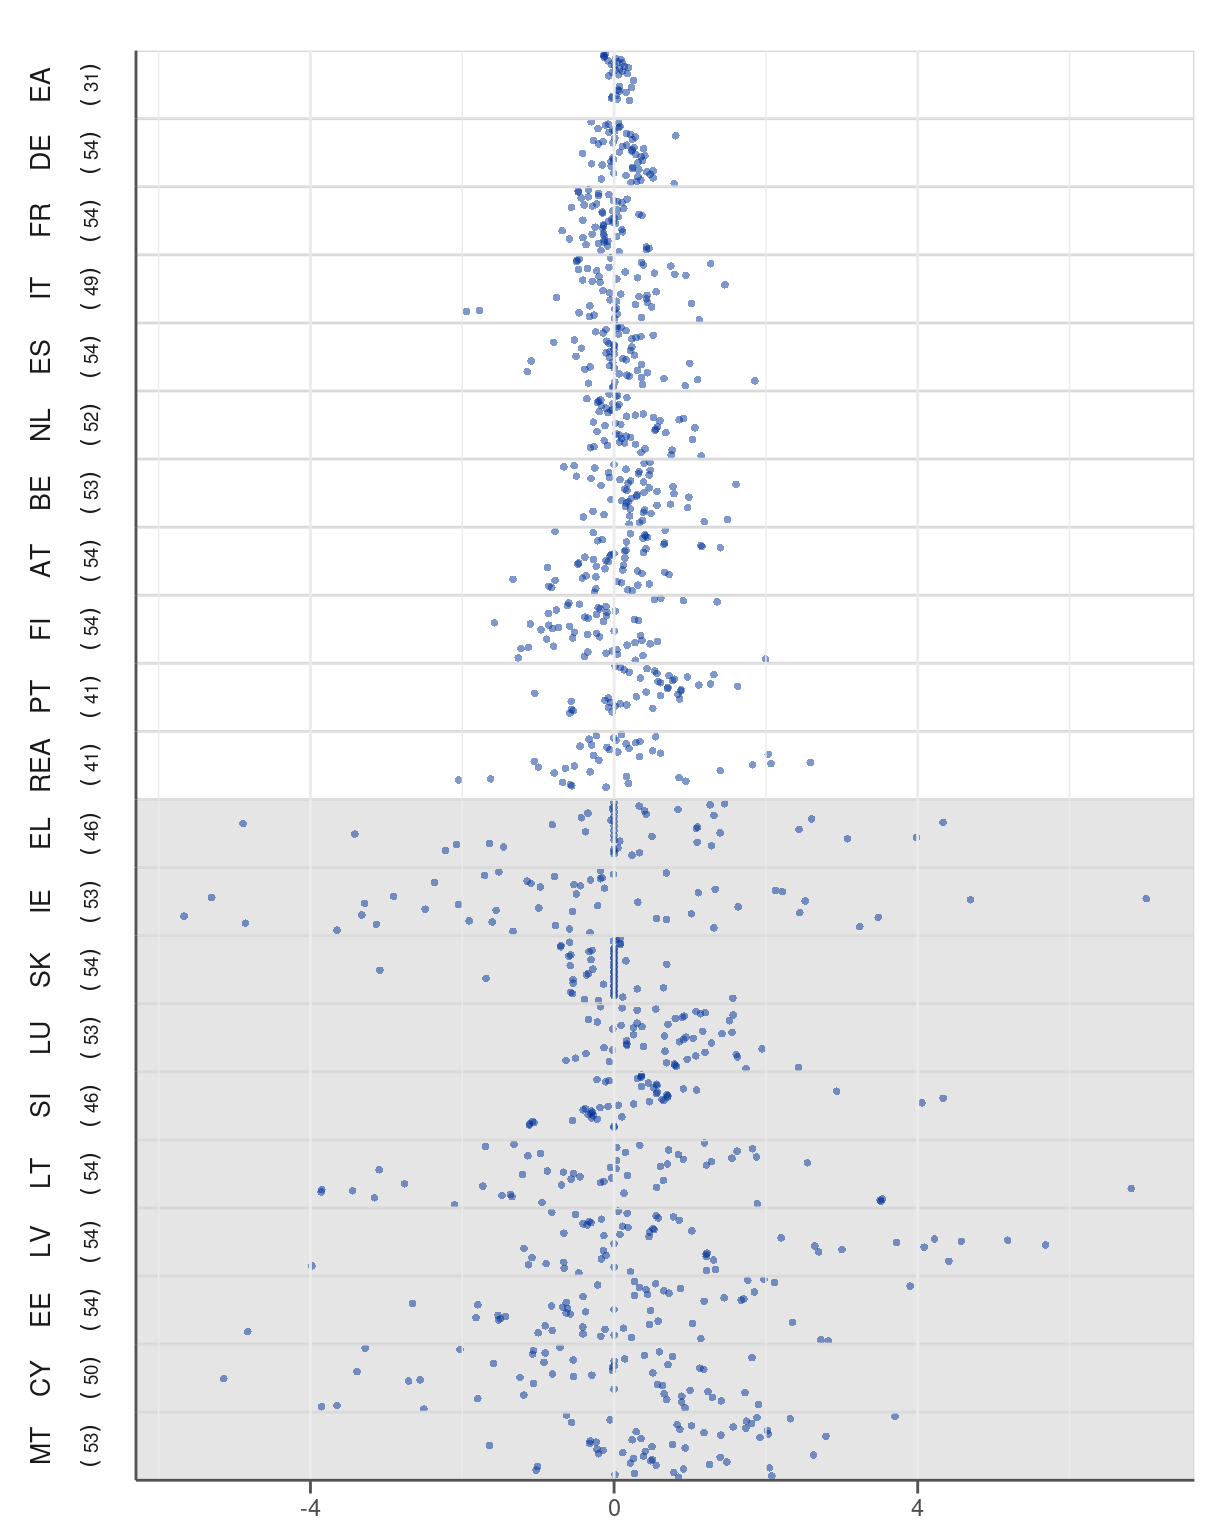
\includegraphics{./A-Graphs-revisions_files/figure-pdf/fig-WGS-1.pdf}

}

\caption{\label{fig-WGS}Final revisions to wages and salaries}

\end{figure}

\hypertarget{sec-fiscal-data-characteristics}{%
\chapter{Selected data
characteristics}\label{sec-fiscal-data-characteristics}}

\begin{figure}[H]

{\centering 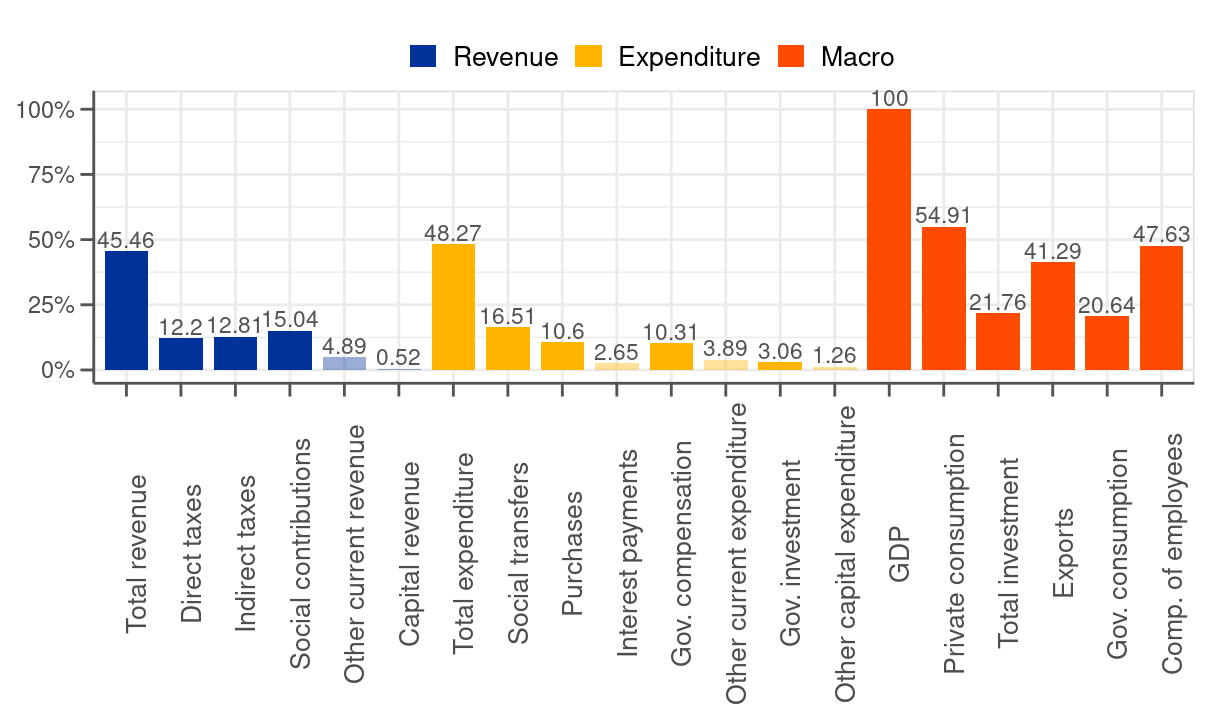
\includegraphics{./B-Fiscal-data_files/figure-pdf/fig-ItemShareGDP-1.pdf}

}

\caption{\label{fig-ItemShareGDP}Average percentage GDP shares across
variables}

\end{figure}

\begin{figure}[H]

{\centering 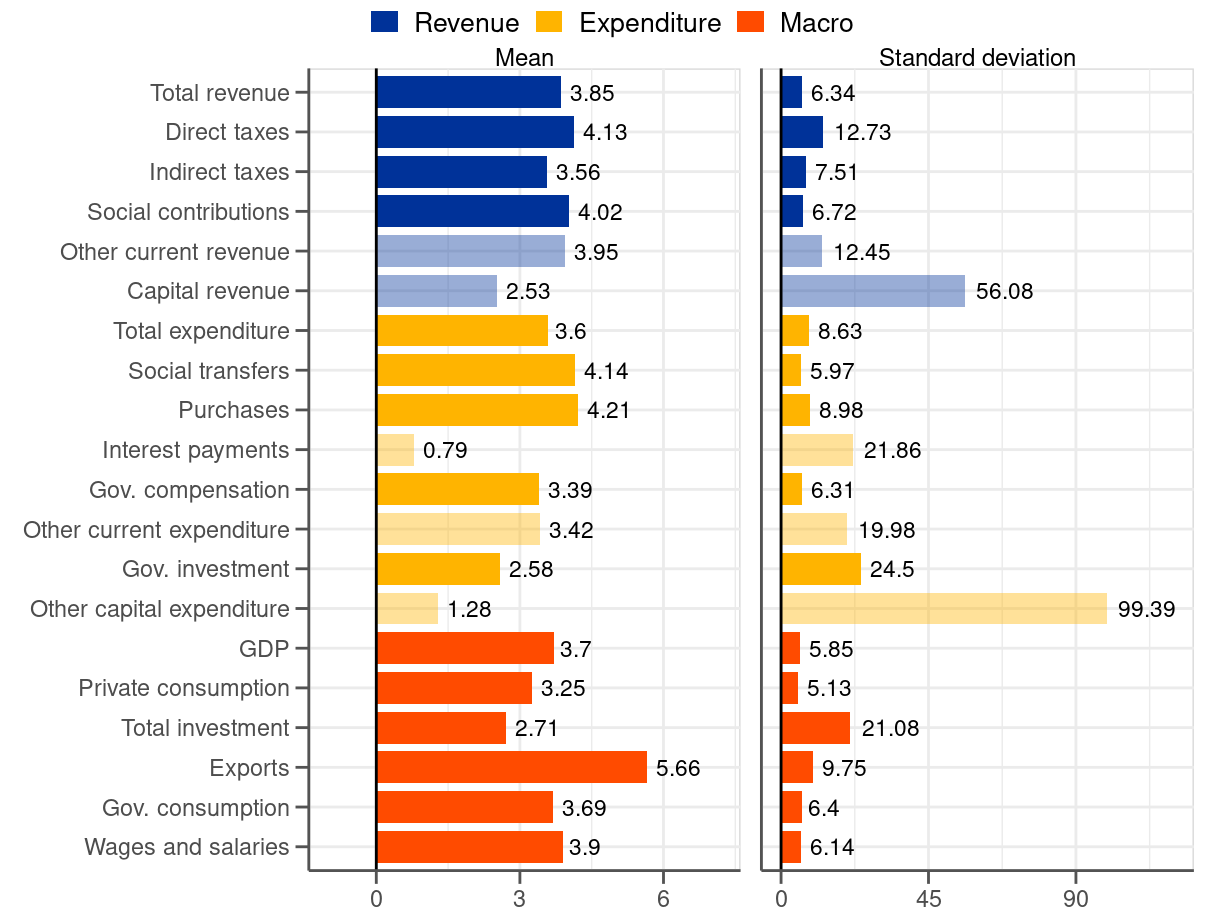
\includegraphics{./B-Fiscal-data_files/figure-pdf/fig-mean-standard-deviation-values-1.pdf}

}

\caption{\label{fig-mean-standard-deviation-values}Mean and standard
deviation of growth rates across variables}

\end{figure}

\begin{figure}[H]

{\centering 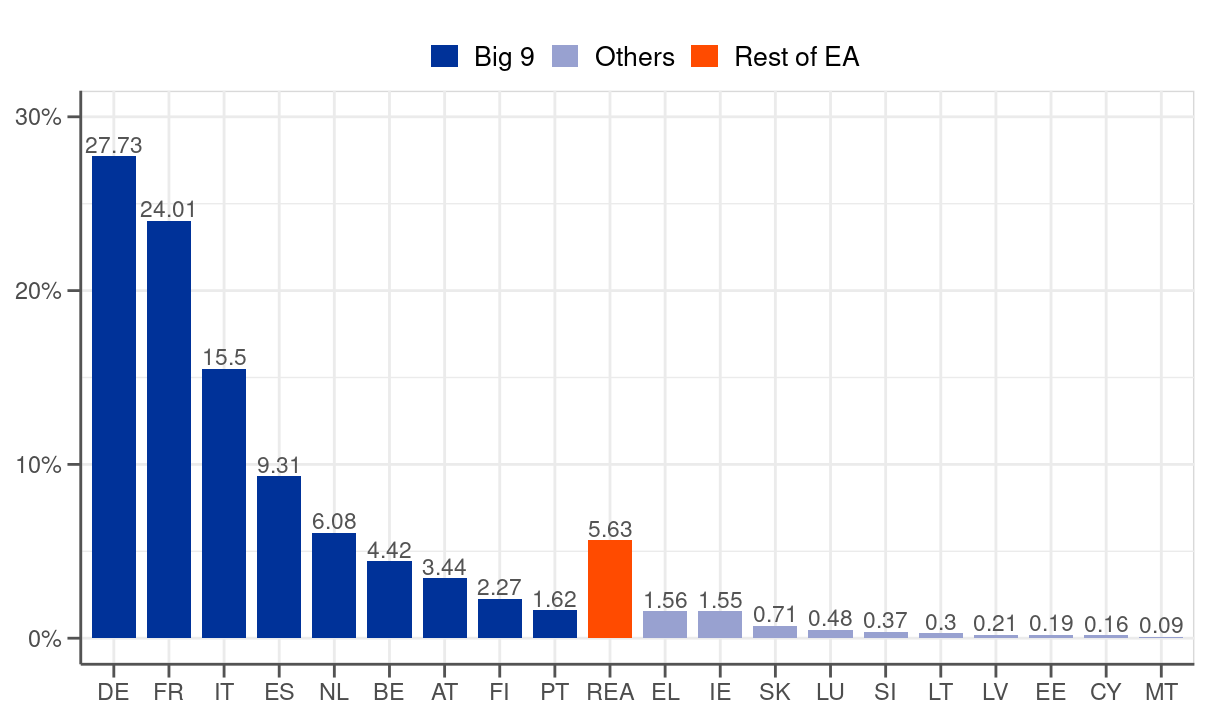
\includegraphics{./B-Fiscal-data_files/figure-pdf/fig-share-TOE-1.pdf}

}

\caption{\label{fig-share-TOE}Average percentage shares of total
expenditure in the euro area}

\end{figure}

\hypertarget{sec-code-retrieval}{%
\chapter{Data codes for retrieval}\label{sec-code-retrieval}}

\hypertarget{tbl-Code-series-fiscal}{}
\begin{table}
\caption{\label{tbl-Code-series-fiscal}ECB's SDW codes for data retrieval (fiscal series) }\tabularnewline

\centering
\begin{tabular}[t]{l|l}
\hline
Name & Retrieval code\\
\hline
Total revenue & GFS.Q.N.cc.W0.S13.S1.P.C.OTR.\_Z.\_Z.\_Z.XDC.\_Z.S.V.N.\_T\\
\hline
Current taxes on income, wealth, etc. (Direct taxes) & GFS.Q.N.cc.W0.S13.S1.N.C.D5.\_Z.\_Z.\_Z.XDC.\_Z.S.V.N.\_T\\
\hline
Taxes on production and imports (Indirect taxes) & GFS.Q.N.cc.W0.S13.S1.N.C.D2.\_Z.\_Z.\_Z.XDC.\_Z.S.V.N.\_T\\
\hline
Net social contributions (Social contributions) & GFS.Q.N.cc.W0.S13.S1.N.C.D61.\_Z.\_Z.\_Z.XDC.\_Z.S.V.N.\_T\\
\hline
Other current revenue = Market output, output for own final use and payments for other non-market output + Other subsidies on production + Property income + Other current transfers & GFS.Q.N.cc.W0.S13.S1.N.C.P1O.\_Z.\_Z.\_Z.XDC.\_Z.S.V.N.\_T +
        GFS.Q.N.cc.W0.S13.S1.N.C.D39.\_Z.\_Z.\_Z.XDC.\_Z.S.V.N.\_T +
        GFS.Q.N.cc.W0.S13.S1.P.C.D4.\_Z.\_Z.\_Z.XDC.\_Z.S.V.N.\_T +
\textcolor[HTML]{b4824b}{\textbf{        GFS.Q.N.cc.W0.S13.S1.P.C.D7.\_Z.\_Z.\_Z.XDC.\_Z.S.V.N.\_T}}\\
\hline
\textcolor[HTML]{b4824b}{\textbf{Capital transfers (Capital revenue)}} & \textcolor[HTML]{b4824b}{\textbf{GFS.Q.N.cc.W0.S13.S1.P.C.D9.\_Z.\_Z.\_Z.XDC.\_Z.S.V.N.\_T}}\\
\hline
Total expenditure & GFS.Q.N.cc.W0.S13.S1.P.D.OTE.\_Z.\_Z.\_T.XDC.\_Z.S.V.N.\_T\\
\hline
Social benefits other than social transfers in kind (Social transfers) & GFS.Q.N.cc.W0.S13.S1.N.D.D62.\_Z.\_Z.\_T.XDC.\_Z.S.V.N.\_T\\
\hline
Purchases = Social transfers in kind - purchased market production + Intermediate consumption & GFS.Q.N.cc.W0.S13.S1.N.D.D632.\_Z.\_Z.\_T.XDC.\_Z.S.V.N.\_T +
        GFS.Q.N.cc.W0.S13.S1.N.D.P2.\_Z.\_Z.\_T.XDC.\_Z.S.V.N.\_T\\
\hline
\textcolor[HTML]{b4824b}{\textbf{Interest (Interest payments)}} & \textcolor[HTML]{b4824b}{\textbf{GFS.Q.N.cc.W0.S13.S1.C.D.D41.\_Z.\_Z.\_T.XDC.\_Z.S.V.N.\_T}}\\
\hline
Compensation of employees (Gov. compensation) & GFS.Q.N.cc.W0.S13.S1.N.D.D1.\_Z.\_Z.\_T.XDC.\_Z.S.V.N.\_T\\
\hline
Other current expenditure = Property income other than interest + Other taxes on production + Current taxes on income, wealth, etc. + Other current transfers + Adjustment for the change in pension entitlements & GFS.Q.N.cc.W0.S13.S1.N.D.D4N.\_Z.\_Z.\_T.XDC.\_Z.S.V.N.\_T +
        GFS.Q.N.cc.W0.S13.S1.N.D.D29.\_Z.\_Z.\_T.XDC.\_Z.S.V.N.\_T +
        GFS.Q.N.cc.W0.S13.S1.N.D.D5.\_Z.\_Z.\_T.XDC.\_Z.S.V.N.\_T +
        GFS.Q.N.cc.W0.S13.S1.P.D.D7.\_Z.\_Z.\_T.XDC.\_Z.S.V.N.\_T +
\textcolor[HTML]{b4824b}{\textbf{        GFS.Q.N.cc.W0.S13.S1.N.D.D8.\_Z.\_Z.\_T.XDC.\_Z.S.V.N.\_T}}\\
\hline
Gross fixed capital formation (Gov. investment) & GFS.Q.N.cc.W0.S13.S1.N.D.P51G.\_Z.\_Z.\_T.XDC.\_Z.S.V.N.\_T\\
\hline
Other capital expenditure = Changes in inventories and acquisition less disposals of valuables + Acquisitions less disposals of non-produced assets + Capital transfers & GFS.Q.N.cc.W0.S13.S1.N.D.P5M.\_Z.\_Z.\_T.XDC.\_Z.S.V.N.\_T +
        GFS.Q.N.cc.W0.S13.S1.N.D.NP.\_Z.\_Z.\_T.XDC.\_Z.S.V.N.\_T +
\textcolor[HTML]{b4824b}{\textbf{        GFS.Q.N.cc.W0.S13.S1.C.D.D9.\_Z.\_Z.\_T.XDC.\_Z.S.V.N.\_T}}\\
\hline
\multicolumn{2}{l}{\rule{0pt}{1em}\textit{Note: }  The items in brown are not explicitly considered in our analysis.}\\
\end{tabular}
\end{table}

\hypertarget{tbl-Code-series-macro}{}
\begin{table}
\caption{\label{tbl-Code-series-macro}ECB's SDW codes for data retrieval (macro series) }\tabularnewline

\centering
\begin{tabular}[t]{l|l}
\hline
Name & Retrieval code\\
\hline
GDP & MNA.Q.N.cc.W2.S1.S1.B.B1GQ.\_Z.\_Z.\_Z.EUR.V.N\\
\hline
Private consumption & MNA.Q.N.cc.W0.S1M.S1.D.P31.\_Z.\_Z.\_T.EUR.V.N\\
\hline
Total investment & MNA.Q.N.cc.W0.S1.S1.D.P5.N1G.\_T.\_Z.EUR.V.N\\
\hline
Exports & MNA.Q.N.cc.W1.S1.S1.D.P6.\_Z.\_Z.\_Z.EUR.V.N\\
\hline
Gov. consumption & MNA.Q.N.cc.W0.S13.S1.D.P3.\_Z.\_Z.\_T.EUR.V.N\\
\hline
Wages and salaries & MNA.Q.N.cc.W2.S1.S1.D.D1.\_Z.\_T.\_Z.EUR.V.N\\
\hline
\end{tabular}
\end{table}


  \bibliography{bibliography.bib}


\end{document}
